%!TEX root = skripsi.tex
%
% Template Laporan Skripsi/Thesis 
%
% @author  Andreas Febrian, Lia Sadita 
% @version 1.03
%
% Dokumen ini dibuat berdasarkan standar IEEE dalam membuat class untuk 
% LaTeX dan konfigurasi LaTeX yang digunakan Fahrurrozi Rahman ketika 
% membuat laporan skripsi. Konfigurasi yang lama telah disesuaikan dengan 
% aturan penulisan thesis yang dikeluarkan UI pada tahun 2008.
%

%
% Tipe dokumen adalah report dengan satu kolom. 
%
\documentclass[12pt, a4paper, onecolumn, oneside, final]{report}

\usepackage{arabtex}
\usepackage{utf8}
\setcode{utf8}
\usepackage{amsmath}
\usepackage{amssymb}
\usepackage{enumitem}
\usepackage{amsmath}
\usepackage{longtable}

\usepackage{algpseudocode}
\algnewcommand\algorithmicinput{\textbf{Input:}}
\algnewcommand\Input{\item[\algorithmicinput]}
\algnewcommand\algorithmicoutput{\textbf{Output:}}
\algnewcommand\Output{\item[\algorithmicoutput]}
\usepackage[ruled,vlined,linesnumbered,resetcount,algochapter]{algorithm2e}
\newcommand{\listofalgorithmes}{\tocfile{\listalgorithmcfname}{loa}}
\renewcommand{\listalgorithmcfname}{Daftar Kode}
\newenvironment{kode}[1][htb]
	{\renewcommand{\algorithmcfname}{Kode}% Update algorithm name
		\begin{algorithm}[#1]%
	}{\end{algorithm}}

\usepackage{natbib}
% Load konfigurasi LaTeX untuk tipe laporan thesis
\usepackage{uithesis}


\newcolumntype{L}[1]{>{\raggedright\let\newline\\\arraybackslash\hspace{0pt}}m{#1}}
\newcolumntype{C}[1]{>{\centering\let\newline\\\arraybackslash\hspace{0pt}}m{#1}}
\newcolumntype{R}[1]{>{\raggedleft\let\newline\\\arraybackslash\hspace{0pt}}m{#1}}
% Load konfigurasi khusus untuk laporan yang sedang dibuat
%!TEX root = skripsi.tex
%-----------------------------------------------------------------------------%
% Informasi Mengenai Dokumen
%-----------------------------------------------------------------------------%
% 
% Judul laporan. 
\var{\judul}{Pengenalan Entitas Kesehatan pada Forum Online dengan Menggunakan Recurrent Neural Networks}
% 
% Tulis kembali judul laporan, kali ini akan diubah menjadi huruf kapital
\Var{\Judul}{Pengenalan Entitas Kesehatan pada Forum Online dengan Menggunakan Recurrent Neural Networks}
% 
% Tulis kembali judul laporan namun dengan bahasa Ingris
\var{\judulInggris}{Medical Entity Recognition on the Online Health Forum using Recurrent Neural Networks}

% 
% Tipe laporan, dapat berisi Skripsi, Tugas Akhir, Thesis, atau Disertasi
\var{\type}{Skripsi}
% 
% Tulis kembali tipe laporan, kali ini akan diubah menjadi huruf kapital
\Var{\Type}{Skripsi}
% 
% Tulis nama penulis 
\var{\penulis}{Wahid Nur Rohman}
% 
% Tulis kembali nama penulis, kali ini akan diubah menjadi huruf kapital
\Var{\Penulis}{Wahid Nur Rohman}
% 
% Tulis NPM penulis
\var{\npm}{1306381856}
% 
% Tuliskan Fakultas dimana penulis berada
\Var{\Fakultas}{Ilmu Komputer}
\var{\fakultas}{Ilmu Komputer}
% 
% Tuliskan Program Studi yang diambil penulis
\Var{\Program}{Ilmu Komputer}
\var{\program}{Ilmu Komputer}
\var{\programEng}{Computer Science}
% 
% Tuliskan tahun publikasi laporan
\Var{\bulanTahun}{Juli 2016}
% 
% Tuliskan gelar yang akan diperoleh dengan menyerahkan laporan ini
\var{\gelar}{Sarjana Ilmu Komputer}
% 
% Tuliskan tanggal pengesahan laporan, waktu dimana laporan diserahkan ke 
% penguji/sekretariat
\var{\tanggalPengesahan}{22 Juli 2016}
% 
% Tuliskan tanggal keputusan sidang dikeluarkan dan penulis dinyatakan 
% lulus/tidak lulus
\var{\tanggalLulus}{27 Juni 2016}
% 
% Tuliskan pembimbing 
\var{\pembimbing}{Dra. Mirna Adriani, Ph.D.}
\var{\pembimbingdua}{Alfan Farizki Wicaksono S.T., M.Sc.}
% 
% Alias untuk memudahkan alur penulisan paa saat menulis laporan
\var{\saya}{penulis}
\var{\Saya}{Penulis}

%-----------------------------------------------------------------------------%
% Judul Setiap Bab
%-----------------------------------------------------------------------------%
% 
% Berikut ada judul-judul setiap bab. 
% Silahkan diubah sesuai dengan kebutuhan. 
% 
\Var{\kataPengantar}{Kata Pengantar}
\Var{\babSatu}{Pendahuluan}
\Var{\babDua}{Landasan Teori}
\Var{\babTiga}{Metodologi}
\Var{\babEmpat}{Eksperimen}
\Var{\babLima}{Hasil Eksperimen dan Analisis}
\Var{\babEnam}{Kesimpulan dan Saran}

% Daftar pemenggalan suku kata dan istilah dalam LaTeX
\usepackage[bahasa]{babel}
\addto\captionsbahasa{\renewcommand\bibname{Daftar Referensi}}
\hyphenrules{bahasa}
%!TEX root = skripsi.tex
%
% Hyphenation untuk Indonesia 
%
% @author  Andreas Febrian
% @version 1.00
% 
% Tambahkan cara pemenggalan kata-kata yang salah dipenggal secara otomatis 
% oleh LaTeX. Jika kata tersebut dapat dipenggal dengan benar, maka tidak 
% perlu ditambahkan dalam berkas ini. Tanda pemenggalan kata menggunakan 
% tanda '-'; contoh:
% menarik
%   --> pemenggalan: me-na-rik
%

\hyphenation{
    % alphabhet A
    a-na-li-sa a-tur 
    a-pli-ka-si 
    % alphabhet B
    ba-ngun-an 
    be-be-ra-pa 
    ber-ge-rak
    ber-ke-lan-jut-an 
    ber-pe-nga-ruh 
    % alphabhet C
    ca-ri
    % alphabhet D
    di-ban-ding-kan
    di-de-fi-ni-si-kan
    di-ha-rap-kan
    di-ka-te-go-ri-kan
    di-mi-li-ki-nya
    di-se-rah-kan
    di-sim-pan di-pim-pin de-ngan da-e-rah di-ba-ngun da-pat di-nya-ta-kan 
    di-sim-bol-kan di-pi-lih di-li-hat de-fi-ni-si
    di-se-su-ai-kan
    % alphabhet E
    e-le-men
    e-ner-gi eks-klu-sif
    % alphabhet F
    fa-si-li-tas
    % alphabhet G
    ga-bung-an ge-rak
    % alphabhet H
    ha-lang-an
    he-te-ro-gen
    % alphabhet I
    i-ngin
    % alphabhet J
    % alphabhet K
    ke-hi-lang-an
    ku-ning 
    kua-li-tas ka-me-ra ke-mung-kin-an ke-se-pa-ham-an
    ke-te-pat-an
    kon-fi-gu-ra-si
    % alphabhet L
    ling-kung-an
    % alphabhet M
    me-min-ta
    me-mo-del-kan
    me-mo-ri
    men-de-fi-ni-si-kan
    me-neng-ah
    meng-a-tas-i me-mung-kin-kan me-nge-na-i me-ngi-rim-kan 
    meng-u-bah meng-a-dap-ta-si me-nya-ta-kan mo-di-fi-ka-si
    meng-a-tur
    meng-au-to-ma-si
    meng-a-ko-mo-da-si
    me-ngo-rek-si
    % alphabhet N
    nya-ta non-eks-klu-sif
    % alphabhet O
    % alphabhet P
    pa-ra-lel
    peng-ala-mat-an
    pen-ting
    penga-da-an
		pe-nye-rap-an 
		pe-ngon-trol
    pe-mo-del-an
    pe-ran  pe-ran-an-nya
    pe-rin-tah
    pem-ba-ngun-an pre-si-den pe-me-rin-tah prio-ri-tas peng-am-bil-an 
    peng-ga-bung-an pe-nga-was-an pe-ngem-bang-an 
    pe-nga-ruh pa-ra-lel-is-me per-hi-tung-an per-ma-sa-lah-an 
    pen-ca-ri-an peng-struk-tur-an
    pe-ner-bang-an
    pro-se-sor
    % alphabhet Q
    % alphabhet R
    ran-cang-an
    % alphabhet S
    se-dang-kan
    se-ring
    si-mu-la-si sa-ngat    
    % alphabhet T
    te-ngah
    ter-da-pat
    % alphabhet U
    u-sa-ha
    % alphabhet V
    % alphabhet W
    % alphabhet X
    % alphabhet Y
    % alphabhet Z
    % special
    MATLAB
    basmalah
    sam-ping
    hardware
    software
    voiced
    overlap
    frame
    bit
    rate
    support
    vector
    machine
    Gaussian
    mixture
    model
    dynamic
    pro-gram-ming
    auto-ma-tically
    mem-ba-ca
    teks-tual
    eks-trak-si
    di-je-las-kan
    be-nar
    sa-lah
    teks-tual
    dengan
    me-re-pre-sen-ta-si
    me-re-pre-sen-ta-si-kan
}
% Daftar istilah yang mungkin perlu ditandai 
%!TEX root = skripsi.tex
%
% @author  Andreas Febrian
% @version 1.00
% 
% Mendaftar seluruh istilah yang mungkin akan perlu dijadikan 
% italic atau bold pada setiap kemunculannya dalam dokumen. 
% 

\var{\license}{\f{Creative Common License 1.0 Generic}}
\var{\bslash}{$\setminus$}
\var{\ioa}{\f{input}}
\var{\iob}{\f{output}}
\var{\br}{\f{bit rate}}
\var{\fr}{\f{frame}}
\var{\quran}{Al-Qur'an}
\var{\mer}{MER}
\var{\rnn}{\f{Recurrent Neural Networks}}
\var{\ol}{\f{online}}
\var{\disease}{\f{disease}}
\var{\symptom}{\f{symptom}}
\var{\drug}{\f{drug}}
\var{\treatment}{\f{treatment}}
\var{\Disease}{\f{Disease}}
\var{\Symptom}{\f{Symptom}}
\var{\Drug}{\f{Drug}}
\var{\Treatment}{\f{Treatment}}
\var{\we}{\f{word embedding}}
\var{\radit}{Raditya Herwando}
\var{\skripsiRadit}{\cite{skripsiKakRadit}}

%\usepackage[backend=bibtex]{biblatex}
%\addbibresource{bib.bib}

% Awal bagian penulisan laporan
\begin{document}
\lefthyphenmin=5
\righthyphenmin=7
%
% Sampul Laporan
%!TEX root = skripsi.tex
%
% Sampul Laporan

%
% @author  unknown
% @version 1.01
% @edit by Andreas Febrian
%

\begin{titlepage}
    \begin{center}    
        \begin{figure}
            \begin{center}
                
\includegraphics[width=2.5cm]{pics/makara.png}
            \end{center}
        \end{figure}    
        \vspace*{0cm}
        \bo{
        	UNIVERSITAS INDONESIA\\
        }
        
        \vspace*{1.0cm}
        % judul thesis harus dalam 14pt Times New Roman
        \bo{\Judul} \\[1.0cm]

        \vspace*{2.5 cm}    
        % harus dalam 14pt Times New Roman
        \bo{\Type}

        \vspace*{3 cm}       
        % penulis dan npm
        \bo{\Penulis} \\
        \bo{\npm} \\

        \vspace*{5.0cm}

        % informasi mengenai fakultas dan program studi
        \bo{
        	FAKULTAS \Fakultas\\
        	PROGRAM STUDI \Program \\
        	DEPOK \\
        	\bulanTahun
        }
    \end{center}
\end{titlepage}


%
% Gunakan penomeran romawi
\pagenumbering{roman}

%
% load halaman judul dalam
\addChapter{HALAMAN JUDUL}
%!TEX root = skripsi.tex
%
% Halaman Judul Laporan 
%
% @author  unknown
% @version 1.01
% @edit by Andreas Febrian
%

\begin{titlepage}
    \begin{center}\begin{figure}
            \begin{center}
                
\includegraphics[width=2.5cm]{pics/makara.png}
            \end{center}
        \end{figure}    
        \vspace*{0cm}
        \bo{
        	UNIVERSITAS INDONESIA\\
        }
        
        \vspace*{1.0cm}
        % judul thesis harus dalam 14pt Times New Roman
        \bo{SEMANTIC ROLE LABELING UNTUK BAHASA INDONESIA PERCAKAPAN DENGAN MENGGUNAKAN DEEP LEARNING} \\[1.0cm]

        \vspace*{2.5 cm}    
        % harus dalam 14pt Times New Roman
        \bo{\Type} \\
        % keterangan prasyarat
        \bo{Diajukan sebagai salah satu syarat untuk memperoleh gelar \\
        \gelar}\\

        \vspace*{3 cm}       
        % penulis dan npm
        \bo{\Penulis} \\
        \bo{\npm} \\

        \vspace*{5.0cm}

        % informasi mengenai fakultas dan program studi
        \bo{
        	FAKULTAS \Fakultas\\
        	PROGRAM STUDI \Program \\
        	DEPOK \\
        	\bulanTahun
        }
    \end{center}
\end{titlepage}

%
% setelah bagian ini, halaman dihitung sebagai halaman ke 2
\setcounter{page}{2}

% sementara ga usah
% load halaman pengesahan
%\addChapter{LEMBAR PERSETUJUAN}
%\documentclass[12pt, a4paper, onecolumn, oneside, final]{report}
\usepackage{pdfpages}
\begin{document}
\includepdf[pages=4]{../skripsi}
\end{document}
%
% load halaman orisinalitas 
\addChapter{LEMBAR PERNYATAAN ORISINALITAS}
%!TEX root = skripsi.tex
%
% Halaman Orisinalitas
%
% @author  Andreas Febrian
% @version 1.01
%

\chapter*{\uppercase{halaman pernyataan orisinalitas}}
\vspace*{2cm}

\begin{center}
	\bo{\type~ini adalah hasil karya saya sendiri, \\ 
	dan semua sumber baik yang dikutip maupun dirujuk \\
	telah saya nyatakan dengan benar.} \\
	\vspace*{2.6cm}
	
	\begin{tabular}{l c l}
	\bo{Nama} & : & \bo{\penulis} \\
	\bo{NPM} & : & \bo{\npm} \\ 
	\bo{Tanda Tangan} & : & \\
	& & \\
	& & \\
	\bo{Tanggal} & : & \bo{\tanggalPengesahan} \\	
	\end{tabular}
\end{center}

\newpage
%
%
\addChapter{LEMBAR PENGESAHAN}
%!TEX root = skripsi.tex
%
% Halaman Pengesahan Sidang
%
% @author  Andreas Febrian, Andre Tampubolon 
% @version 1.02
%

\chapter*{HALAMAN PENGESAHAN}

\vspace*{0.4cm}
\noindent 

\noindent
\begin{tabular}{ll p{9cm}}
	\type~ini diajukan oleh&: & \\
	Nama&: & \penulis \\
	NPM&: & \npm \\
	Program Studi&: & \program \\
	Judul \type&: & \judul \\
\end{tabular} \\

\vspace*{1.0cm}

\noindent \bo{Telah berhasil dipertahankan di hadapan Dewan Penguji 
dan diterima sebagai bagian persyaratan yang diperlukan untuk 
memperoleh gelar \gelar~pada Program Studi \program, Fakultas 
\fakultas, Universitas Indonesia.}\\[0.2cm]

\begin{center}
	\bo{DEWAN PENGUJI}
\end{center}

\vspace*{0.3cm}

\begin{tabular}{l l l l }
	& & & \\
	Pembimbing 1&: & \pembimbing & (\hspace*{3.0cm}) \\
	& & & \\
	Pembimbing 2&: & \pembimbingdua & (\hspace*{3.0cm}) \\
	& & & \\
	Penguji&: & - & (\hspace*{3.0cm}) \\
	& & & \\
	Penguji&: & - & (\hspace*{3.0cm}) \\
\end{tabular}\\

\vspace*{2.0cm}

\begin{tabular}{ll l}
	Ditetapkan di&: & Depok\\
	Tanggal&: & \tanggalLulus \\
\end{tabular}


\newpage
%
%
\addChapter{\kataPengantar}
%!TEX root = skripsi.tex
%-----------------------------------------------------------------------------%
\chapter*{\kataPengantar}
%-----------------------------------------------------------------------------%

Segala puji bagi Allah, Tuhan semesta alam, semoga keselamatan dan kesejahteraan tetap terlimpahkan atas junjungan kita Nabi Muhammad SAW, sebaik-baik teladan bagi umat manusia. Segala puji dan syukur kehadirat Allah SWT, Tuhan Yang Maha Esa, yang telah memberikan pertolongan, sehingga \saya~dapat menyelesaikan skripsi ini.

Penulisan skripsi ini ditujukan untuk memenuhi salah satu syarat untuk menyelesaikan pendidikan pada Program \gelar, Universitas Indonesia. \Saya~sadar bahwa dalam perjalanan menuntut ilmu di universitas hingga dalam menyelesaikan skripsi ini, \saya~tidak sendiri. \Saya~ingin berterima kasih kepada pihak-pihak yang selalu peduli, mendampingi, dan mendukung \saya, yaitu:

\begin{enumerate}
	\item Kedua Orang Tua \saya~yang selalu memberikan dukungan dan do'a kepada \saya.
	\item Dra. Mirna Adriani, Ph.D. dan Alfan Farizki Wicaksono S.T., M.Sc. selaku dosen pembimbing yang banyak memberikan arahan, masukan, dan bantuan dalam menyelesaikan skripsi ini.
  \item Rahmad Mahendra, S.Kom., M.Sc. yang telah memberikan banyak masukan dan saran dalam menyelesaikan skripsi ini.
  \item Andreas Febrian yang telah membuat \f{template} dokumen skripsi ini, sehingga \saya~menjadi terbantu dalam menulis skripsi.
  \item Erik Dominikus yang telah mempublikasikan dan mempopulerkan \f{template} dokumen skripsi ini, sehingga \saya~menjadi tahu bahwa ada \f{template} tersebut.
  \item Alfan Nur Fauzan yang telah memberikan \f{template} dokumen skripsi yang telah diperbaiki ini, sehingga saya sangat terbantu dalam melakukan penulisan
	\item Putu Wira Astika Dharma, Andi Fajar Nur Ismail dan Ken Nabila Setya, sebagai rekan yang banyak memberi masukan dan berbagi ide dengan \saya.
  \item Teman-teman Lab Information Retrieval yang memberi dukungan dan semangat kepada \saya~untuk menyelesaikan skripsi ini.
  \item Segenap teman-teman angkatan 2013 (Angklung) yang memberi dukungan dan semangat kepada \saya~untuk menyelesaikan skripsi ini.
	\item Pihak-pihak lain yang tidak dapat \saya~sebutkan satu-persatu yang sudah memberikan bantuan dan dukungannya kepada \saya.
\end{enumerate}
\vspace*{0.1cm}
\begin{flushright}
Depok, Desember 2017\\[0.1cm]
\vspace*{1cm}
\penulis

\end{flushright}
%
%
\addChapter{LEMBAR PERSETUJUAN PUBLIKASI ILMIAH}
%!TEX root = skripsi.tex
% 
% @author  Andre Tampubolon, Andreas Febrian
% @version 1.01
% 

\chapter*{\uppercase{Halaman Pernyataan Persetujuan Publikasi Tugas Akhir untuk Kepentingan Akademis}}

\vspace*{0.2cm}
\noindent 
Sebagai sivitas akademik Universitas Indonesia, saya yang bertanda 
tangan di bawah ini:
\vspace*{0.4cm}


\begin{tabular}{p{4.2cm} l p{6cm}}
	\bo{Nama} & : & \penulis \\ 	
	\bo{NPM} & : & \npm \\
	\bo{Program Studi} & : & \program\\	
	\bo{Fakultas} & : & \fakultas\\
	\bo{Jenis Karya} & : & \type \\
\end{tabular}

\vspace*{0.6cm}
\noindent demi pengembangan ilmu pengetahuan, menyetujui untuk memberikan 
kepada Universitas Indonesia \bo{Hak Bebas Royalti Noneksklusif 
(Non-exclusive Royalty Free Right)} atas karya ilmiah saya yang berjudul:
\begin{center}
	\judul
\end{center}
beserta perangkat yang ada (jika diperlukan). Dengan Hak Bebas Royalti 
Noneksklusif ini Universitas Indonesia berhak menyimpan, 
mengalihmedia/formatkan, mengelola dalam bentuk pangkalan data 
(\f{database}), merawat, dan memublikasikan tugas akhir saya selama 
tetap mencantumkan nama saya sebagai penulis/pencipta dan sebagai 
pemilik Hak Cipta. \\

\noindent Demikian pernyatan ini saya buat dengan sebenarnya.

\begin{center}
	\vspace*{0.8cm}
	\begin{tabular}{lll}
		Dibuat di&: & Depok \\
		Pada tanggal&: & \tanggalPengesahan \\
	\end{tabular}\\

	\vspace*{0.2cm}
	Yang menyatakan \\
	\vspace*{2cm}
	(\penulis)
\end{center}

\newpage


%
% 
\singlespacing
\addChapter{ABSTRAK}
%!TEX root = skripsi.tex
%
% Halaman Abstrak
%
% @author  Andreas Febrian
% @version 1.00
%

\chapter*{Abstrak}

\vspace*{0.2cm}

\noindent \begin{tabular}{l l p{10cm}}
	Nama&: & \penulis \\
	Program Studi&: & \program \\
	Judul&: & Semantic Role Labeling untuk Bahasa Indonesia Percakapan dengan Menggunakan Deep Learning \\
\end{tabular} \\ 

\vspace*{0.5cm}

\noindent 

\textit{Semantic Role Labeling} (SRL) telah diteliti cukup dalam, terutama untuk Bahasa Inggris yang formal. Akan tetapi, hanya terdapat sedikit riset untuk bahasa percakapan informal, terutama untuk bahasa yang digunakan dalam sistem \textit{chatbot}. Dalam Bahasa Indonesia, kedua jenis bahasa formal dan percakapan masih sedikit diteliti untuk membangun sistem SRL. Pada riset ini, kami berfokus pada menyelesaikan permasalahan SRL untuk Bahasa Indonesia percakapan. Kontribusi kami adalah memperkenalkan set \textit{semantic roles} baru dan mengajukan \textit{attention mechanism} di atas arsitektur \textit{Long Short-Term Memory Networks}. Tantangan dalam Bahasa Indonesia percakapan adalah \textit{slang} dan singkatan, kalimat pendek, dan struktur yang tidak beraturan. Walaupun riset ini merupakan \textit{pilot task}, kami memperoleh hasil yang menjanjikan dengan nilai F1 82.68\%.


\vspace*{0.2cm}

\noindent Keywords: \\ 
\noindent Semantic Role Labeling, deep learning, bahasa percakapan, RNNs \\ 

\newpage
%
%
%!TEX root = skripsi.tex
%
% Halaman Abstract
%
% @author  Andreas Febrian
% @version 1.00
%

\chapter*{ABSTRACT}

\vspace*{0.2cm}

\noindent \begin{tabular}{l l p{11.0cm}}
	Name&: & \penulis \\
	Program&: & \programEng \\
	Title&: & \judulInggris \\
\end{tabular} \\ 

\vspace*{0.5cm}

\noindent 

Nowadays, everyone can use online health forums for seeking information regarding health issues without directly visiting a doctor in the hospital. There are thousands of health-related posts generated by thousands of online users everyday. As a result, A huge amount of information can be extracted from such online forums. In this work, we focus on seeking a good computational model to automatically extract the names of disease, symptom, treatment, and drug due to its usefulness for future task, such as Medical Question Answering systems. Furthermore, we formulate our problem as a sequence labeling problem using machine learning approach. We propose Deep Learning technique using Recurrent Neural Networks (RNNs), because RNNs is state-of-the-art for sequence labeling problem. We propose some features such as word features, medical dictionary, stop word, POS-Tag, word phrase(verb and noun), word before and word after. Furthermore we propose two RNNs architectures, which are LSTMs in one layer and LSTMs in two layer with multi-input. The result of this experiment shows that the model proposed can give the good result. Based on the experiment using the combination features of its own word, medical dictionary, stop word, word phrase (noun and verb), 1 word before and 1 word after using the first RNNs architecture achieve f-measure $ 63.06\% $, and using second RNNs architecture achieve f-measure $ 62.14\% $. Thats result is better than the baseline used \citep{skripsiKakRadit}, f-measure $ 54.09\% $.


\vspace*{0.2cm}

\noindent Keywords: \\ 
\noindent \mer, RNNs, disease, symptom, treatment, drug \\ 

\newpage

%
% Daftar isi, gambar, dan tabel
%
\tableofcontents
\clearpage
\listoffigures
\clearpage
\listoftables
\clearpage
\listofalgorithmes
% \lstlistoflistings
\clearpage

%
% Gunakan penomeran Arab (1, 2, 3, ...) setelah bagian ini.
%
\pagenumbering{arabic}

%
%
%
\onehalfspacing
%!TEX root = skripsi.tex
%-----------------------------------------------------------------------------%
\chapter{\babSatu}
%-----------------------------------------------------------------------------%


%-----------------------------------------------------------------------------%
\section{Latar Belakang}
%-----------------------------------------------------------------------------%
	
	Saat ini, perkembangan teknologi semakin mempermudah berbagai kegiatan manusia yang dilakukan sehari-hari. Sebagai contoh, ketika seseorang mengalami permasalahan kesehatan dan ingin berkonsultasi kepada para dokter, ia dapat memanfaatkan forum kesehatan \textit{online} yang dapat memungkinkan terjadinya interaksi antara pasien dan dokter tanpa perlu tatap muka.  Melalui forum tersebut, seseorang hanya perlu menuliskan keluhan dan pertanyaan pada formulir yang tersedia. Kemudian, dokter yang memiliki akun di forum kesehatan \textit{online} tersebut dapat memberikan jawaban atas pertanyaan orang tersebut.
	
	Banyak sekali informasi bermanfaat yang dapat diperoleh dari forum kesehatan \textit{online}. Informasi tersebut meliputi informasi keluhan yang dialami pasien, obat yang sebaiknya digunakan atau langkah penyembuhan yang dapat dilakukan. Orang lain dapat mencari obat atau langkah penyembuhan dari forum tersebut melalui pertanyaan yang sudah diajukan sebelumnya. Oleh karena itu, akan sangat baik apabila ada sebuah model atau sistem yang mampu mengekstrak secara otomatis informasi-informasi tersebut. Tantangan utama dari pengembangan model ini adalah \textit{post} atau isi dari forum yang tidak terstruktur. Dokumen \textit{post} tidak dibagi menjadi beberapa bagian seperti bagian keluhan, penyakit, obat dan lain sebagainya, namun hanya menjadi satu bagian saja. Misalnya ketika seseorang menanyakan tentang keluhannya, orang tersebut hanya diberikan dua buah isian berupa judul dan isi pertanyaan. Jawaban yang diberikan oleh dokter juga sama, hanya menjadi satu bagian saja. Jawaban yang diberikan tidak terstruktur seperti memiliki bagian langkah penyembuhan, nama penyakit dan obat secara terpisah. Hal ini menyebabkan orang sulit melakukan ekstraksi informasi dari dokumen tersebut.
	
	Dari permasalahan tersebut, terdapat sebuah solusi untuk melakukan ekstraksi informasi penyakit dalam suatu dokumen, yaitu dengan menggunakan sistem Pengenalan Entitas Kesehatan (\textit{Medical Entity Recognition}) atau disingkat MER. Sistem \mer~ini dapat mengenali entitas kesehatan dalam sebuah dokumen. Apabila diberikan sebuah dokumen, sistem ini akan mengembalikan dokumen yang telah mendapatkan label pada masing-masing entitas kesehatan di dalamnya.
	
	Penelitian dalam rangka mengembangkan sistem \mer~sudah banyak dilakukan oleh beberapa peneliti. Salah satu penelitian tersebut dilakukan oleh \cite{abacha2011medical} dengan menggunakan dokumen medis rumah sakit berbahasa Inggris. Entitas yang mendapatkan label pada penelitian tersebut adalah \textit{treatment}, \textit{problem} dan \textit{test}. Terdapat tiga pendekatan yang digunakan, yaitu pendekatan \textit{machine learning}, pendekatan \textit{rule based} dan pendekatan \textit{hybrid}. Kesimpulan yang dicapai pada penelitian tersebut adalah pendekatan \textit{hybrid} memberikan hasil terbaik, yaitu dengan \textit{precision} $ 72.18\% $, \textit{recall} $ 83.78\% $ dan \textit{F-Measure} $ 77.55\% $.
		
	Pada dokumen berbahasa Indonesia, pengembangan sistem \mer~masih belum banyak dilakukan. Ada beberapa penelitian terkait sistem \mer, namun hasil yang diberikan belum memuaskan. Salah satu penelitian terkait \mer~dilakukan oleh \cite{skripsiKakRadit} yang menggunakan dokumen forum kesehatan \textit{online} berbahasa Indonesia dari beberapa situs. Tujuan dari penelitian tersebut adalah untuk mencari kombinasi fitur yang dapat menghasilkan akurasi terbaik. \cite{skripsiKakRadit} menggunakan algoritma \textit{Conditional Random Fields} dengan hasil akhir yaitu \textit{precission}~70.97\%, \textit{recall}~57.83\% dan \textit{f-measure}~63.69\%. Fitur-fitur yang membuat model memiliki akurasi terbaik yaitu fitur kata itu sendiri, frasa, kamus (\textit{symptom, disease, treatment, drug}), \textit{window feature (previous word)} dan panjang kata.
	
	Dalam penelitian ini \saya~memandang permasalahan pelabelan dokumen kesehatan sebagai permasalahan \textit{sequence labeling}. \Saya~mengusulkan penggunaan teknik \textit{Deep Learning} dengan menggunakan \textit{Recurrent Neural Networks} (RNNs), karena RNNs merupakan \textit{state-of-the-art} untuk permasalahan \textit{sequence labeling} seperti permasalahan pada penelitian ini. Sebelumnya penelitian terkait hal ini pernah dikerjakan oleh \cite{mujiono2016new}, dengan jenis entitas yang digunakan adalah entitas \textit{Drug} saja. Peneliti tersebut menggunakan model RNNs untuk melabeli dokumen secara otomatis. Dengan menggunakan fitur vektor kata yang menggunakan \textit{word embedding} saja, \textit{f-measure} yang diberikan mencapai 86.45\%. Oleh karena itu, \saya~mengusulkan model RNNs pada penelitian ini.
		
	\Saya~berharap bahwa penelitian ini akan memberikan banyak manfaat. Sistem \mer~yang dihasilkan dapat digunakan untuk membuat aplikasi lain. Misalnya dengan adanya \mer~pada dokumen bahasa Indonesia, dapat dibuat sistem untuk melakukan \textit{indexing} dokumen forum sehingga pencarian dokumen kesehatan dapat dilakukan dengan lebih efisien. Selain itu, keluaran dari \mer~juga dapat digunakan untuk mengidentifikasi tren penyakit pada waktu tertentu dari suatu sumber, sehingga pihak terkait mampu melakukan langkah dan kebijakan yang tepat. Sistem \mer~juga dapat digunakan pada aplikasi \textit{Question Answering} \citep{abacha2011medical} dengan cara memanfaatkan hasil pelabelan untuk melakukan identifikasi entitas yang ditanyakan. Gambar \ref{fig:merforqa} merupakan contoh penggunaan \mer~pada aplikasi \textit{question answering} dalam bidang kesehatan.
	
	\begin{figure}
		\centering
		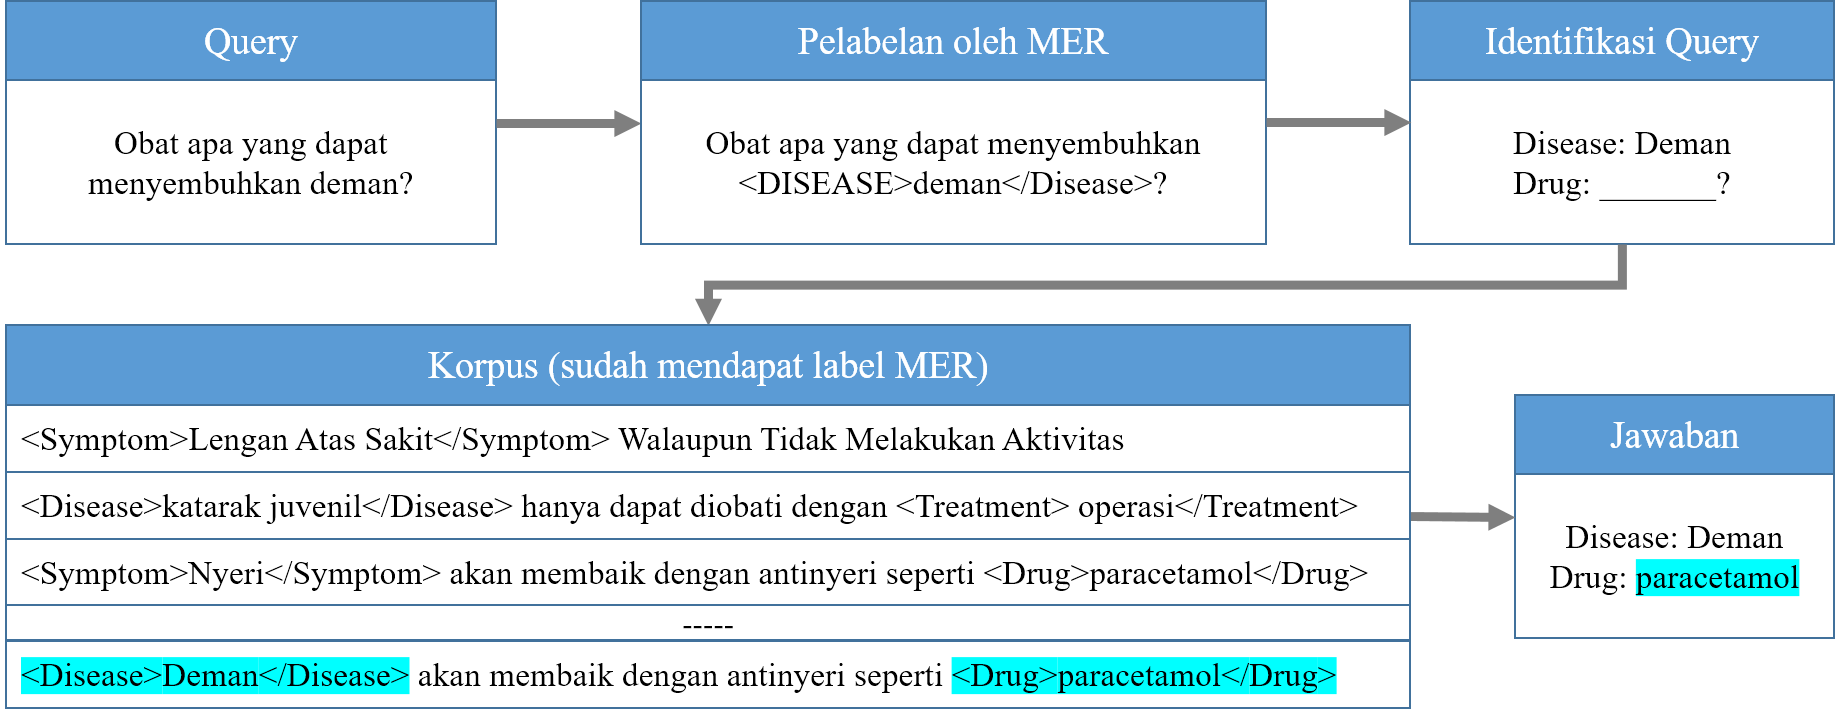
\includegraphics[width=\linewidth]{images/merforqa}
		\caption{Diagram Penggunaan MER pada aplikasi \textit{Question Answering}}
		\label{fig:merforqa}
	\end{figure}
	
	\Saya~berharap bahwa penelitian \mer~pada dokumen berbahasa Indonesia ini dapat dilanjutkan sehingga dapat menghasilkan model yang lebih baik dan membuat suatu aplikasi yang memanfaatkan keluaran dari penelitian ini. Masih banyak manfaat lain yang didapatkan dengan adanya sistem \mer~yang memiliki hasil akurat. 

%-----------------------------------------------------------------------------%
\section{Perumusan Masalah}
%-----------------------------------------------------------------------------%
Berdasarkan latar belakang di atas, dalam penelitian ini \saya~ mengajukan rumusan masalah sebagai berikut:
\begin{enumerate}
	% Bagaimana --- %
	\item Bagaimana performa RNNs dibandingkan dengan CRFs (\textit{baseline}) untuk sistem \mer~yang dikembangkan?
	\item Fitur apa saya yang membuat sistem \mer~memiliki performa terbaik?
\end{enumerate}

%-----------------------------------------------------------------------------%
\section{Tujuan dan Manfaat Penelitian}
%-----------------------------------------------------------------------------%
Penelitian ini bertujuan untuk membangun sistem yang mampu melakukan ekstraksi entitas kesehatan dari forum \textit{online}. Sebenarnya, pada penelitan yang dilakukan oleh \cite{skripsiKakRadit} sudah menghasilkan sebuah sistem yang sama. Namun, fokus penelitian ini yaitu mencoba menggunakan metode yang berbeda. Metode tersebut yaitu dengan menggunakan RNNs dengan harapan mampu memberikan hasil yang lebih baik. Penelitian ini juga bertujuan untuk mendapatkan fitur-fitur yang membuat sistem memiliki performa terbaik. Selain itu, penelitian ini juga bertujuan untuk mendapatkan informasi baru terkait pembuatan sistem \mer~berbahasa Indonesia.

Manfaat dari penelitian ini adalah menghasilkan rancangan sistem dan metode yang dapat digunakan sebagai bahan penelitian lanjutan. Saat ini, sistem dan metode yang dihasilkan hanya mampu mengenali entitas kesehatan saja. Hal ini dapat digunakan untuk membuat sistem informasi tentang suatu jenis penyakit lengkap dengan gejala, obat dan cara penyembuhannya. Selama ini, masyarakat yang menanyakan suatu penyakit melalui forum \ol~tidak membaca terlebih dahulu riwayat pertanyaan yang telah ditanyakan oleh orang lain. Oleh karena itu, diharapkan dengan sistem informasi tersebut, calon penanya hanya perlu mencari penyakit yang akan ditanyakan pada sistem informasi tersebut. Apabila tidak ada, penanya dapat mengajukan pertanyaan, kemudian pertanyaan dan jawaban yang diberikan akan terindeks oleh sistem dan menambah informasi. 

Selain itu, hasil penelitian ini juga dapat digunakan untuk membangun sistem yang mengenali tren penyakit pada masyarakat, sehingga pihak terkait mampu menentukan langkah strategis yang tepat. Sistem \mer~juga dapat digunakan pada aplikasi \textit{Question Answering} \citep{abacha2011medical} dengan cara memanfaatkan hasil pelabelan untuk melakukan identifikasi entitas yang ditanyakan.

%-----------------------------------------------------------------------------%
\section{Metodologi Penelitian}
%-----------------------------------------------------------------------------%
Berikut merupakan metode penelitian yang \saya~lakukan.
\begin{enumerate}
	\item Studi Literatur\\
	Pada tahapan ini \saya~mencari literatur yang terkait dengan penelitian ini. Literatur ini digunakan sebagai bahan pemelajaran dan untuk mendukung penelitian yang \saya~lakukan. Literatur yang \saya~gunakan memiliki keterkaitan terhadap kasus \mer, \textit{Sequence Labeling} dan \rnn.
	
	\item Pengumpulan Data \\
	Pada tahapan ini, \saya~mengumpulkan data percobaan yang diperlukan. \Saya~mengumpulkan dokumen teks dari forum kesehatan \textit{online} dan dari penelitian \cite{skripsiKakRadit}. Setelah dokumen terkumpul, \saya~melakukan langkah-langkah pra-pemrosesan baik pada dokumen yang \saya~dapatkan dari forum maupun korpus dari penelitian \cite{skripsiKakRadit}. Tujuan langkah tersebut yaitu untuk menghilangkan beberapa karakter yang mengganggu tahapan selanjutnya, melakukan normalisasi pada beberapa kasus token, dan lain sebagainya. Setelah itu \saya~melakukan tokenisasi dan melakukan pemecahan kalimat dengan menggunakan beberapa aturan, kemudian \saya~memberikan label pada dokumen yang \saya~dapat dari forum secara manual. 
	
	\item Pengembangan Model\\
	Pada tahapan ini, \saya~melakukan perancangan eksperimen yang akan dilakukan. \Saya~mendefinisikan fitur-fitur yang akan diuji pada penelitian ini dan arsitektur RNNs yang juga akan diuji.
		
	\item Eksperimen \\
	Tahapan ini merupakan bagian inti dari penelitian. \saya~melakukan langkah eksperimen dengan tujuan mendapatkan jawaban dari pertanyaan yang telah dirumuskan pada rumusan masalah. Sebelum masuk di tahap ini, \saya~melakukan pemecahan data menjadi 10 bagian untuk mengimplementasikan \textit{10-cross fold validation}. Setelah itu, data disusun sedemikian sehingga siap digunakan sebagai \textit{resource} eksperimen.
	
	\item Evaluasi dan Analisis Hasil \\
	Pada tahapan ini \saya~melakukan evaluasi dan analisis dari hasil eksperimen. Untuk mengukur akurasi dari masing-masing fitur dan arsitektur RNNs yang \saya~usulkan, saya menggunakan \textit{precision}, \textit{recall} dan \textit{f-measure}.
		
	\item Penarikan Kesimpulan \\
	Tahap ini merupakan tahap terakhir dari penelitian. Setelah melakukan serangkaian eksperimen, evaluasi dan analisis, \saya~memberikan kesimpulan dan informasi penting terkait penelitian ini. Selain itu \saya~juga memberikan saran untuk penelitian selanjutnya.
\end{enumerate}

%-----------------------------------------------------------------------------%
\section{Ruang Lingkup Penelitian}
Pada penelitian ini terdapat beberapa batasan yang \saya~tentukan, yaitu:
\begin{enumerate}
\item{\bf Entitas Kesehatan}\\
Pengenalan entitas kesehatan pada penelitian ini berfokus pada pengenalan nama penyakit (\disease), gejala-gejala penyakit (\symptom), nama obat (\drug) dan langkah pengobatan (\treatment),

\item{\bf Domain Pengenalan}\\
Pengenalan entitas kesehatan dilakukan pada bagian judul pertanyaan, isi pertanyaan/keluhan dan isi jawaban dari dokter.
\end{enumerate}

%-----------------------------------------------------------------------------%

%-----------------------------------------------------------------------------%
\section{Sistematika Penulisan}
%-----------------------------------------------------------------------------%
Sistematika penulisan dalam laporan penelitian ini sebagai berikut:
\begin{itemize}

	\item Bab 1 \babSatu \\
	Pada bab ini \saya~menjelaskan mengenai motivasi dalam melakukan penelitian ini dan komponen-komponen utama penelitian seperi latar belakang, perumusan masalah, tujuan dan manfaat penelitian, metodologi penelitian, ruang lingkup penelitian dan sistematika penulisan.
	
	\item Bab 2 \babDua \\
	Pada bab ini \saya~melakukan studi literatur mengenai beberapa teori dan penelitian yang dilakukan oleh penulis lain. 
		
	\item Bab 3 \babTiga \\
	Pada bab ini \saya~menjelaskan alur dari penelitian ini, yaitu pengumpulan data, pra-pemrosesan, pelabelan, pengembangan model, eksperimen dan evaluasi.
		
	\item Bab 4 \babEmpat \\
	Pada bab ini \saya~menjelaskan proses implementasi sistem dan eksperimen berdasarkan rancangan yang telah \penulis~tentukan pada bab sebelumnya. Selain itu \saya~juga menjelaskan implementasi dari masing-masing tahapan yang dilakukan.
		
	\item Bab 5 \babLima \\
	Pada bab ini \saya~menjelaskan analisis dari hasil eksperimen yang telah \saya~kerjakan pada tahap sebelumnya. Hasil eksperimen \saya~sajikan dalam bentuk tabel dan grafik.
	
	\item Bab 6 \babEnam \\
	Pada bab ini \saya~memberikan kesimpulan berdasarkan hasil eksperimen dan analisis yang telah dilakukan pada penelitian ini. Selain itu \saya~juga memberikan saran dan masukan untuk penelitian dan pengembangan sistem mengenai \mer~berbahasa Indonesia selanjutnya.
	
\end{itemize}
%!TEX root = skripsi.tex
%-----------------------------------------------------------------------------%
\chapter{\babDua}
This chapter focuses on the literature study of three aspects including language models, deep learning, and semantic role labeling. In language model section, Part-of-Speech tag (POS tag) and word embedding are described. Deep learning section focuses on the architecture widely used for sequence labeling problem. Finally, we explain semantic role labeling in the last section, including the semantic roles definition, annotation corpus, common features, and the historical perspectives.
%-----------------------------------------------------------------------------%
%-----------------------------------------------------------------------------%
\section{Language Models}
This section explains the language models usually used in Natural Language Processing (NLP) applications as the features. We first describe the traditional yet important language model, Part-of-Speech tag (POS tag), followed by the so-called word embedding that is often used in recent NLP systems.

\subsection{Part-of-Speech Tag (POS Tag)}
Part-of-Speech (POS) tag defines the class of a word. Some examples of POS tag are noun, verb, adverb, and adjective. POS tags are useful because of the large amount of information they give about a word and its neighbors~\citep{jurafsky2016speech}. For instance, knowing whether a word is a noun tells us about likely neighboring words since nouns are usually preceded by determiners or adjectives. It also tells us about the syntactic structure around the word as nouns are generally part of noun phrases. Table~\ref{tab:examplepostheory} shows an example of a sentence and the POS tags for each word. PRP, VBP, DET, and NN refer to personal pronoun, present verb, determiner, and singular noun, respectively.

\begin{table}
	\centering
	\caption{An example of a sentence and the POS tags for each word}
	\label{tab:examplepostheory}
	\begin{tabular}{|lccccc|}
		\hline
		\textbf{Sentence} 				& I & eat & a &chicken & rice \\
		\hline
		\textbf{POS tag}		& PRP & VBP & DET & NN & NN \\
		\hline
	\end{tabular}
\end{table}

The computational methods for assigning POS tags to words is called POS tagging~\citep{jurafsky2016speech}. POS tagging can be trained using supervised approaches such as Hidden Markov Model and the Maximum Entropy Markov Model~\citep{jurafsky2016speech}.
 

\subsection{Word Embedding}
Word representation is an important feature when one wants to build a model for NLP tasks. The idea is to convert words into vectors. There are two approaches for this vector representation, which are traditional and word embedding approach. Traditional approach uses one-hot vectors for the representation, meanwhile word embedding approach uses real values vectors that contain information about the words~\citep{mikolov2013efficient}.

In the traditional approach, the vectors are retrieved based on the index of the word found in the dictionary. The dictionary consists of the word and its index. Suppose that we have four words: \textit{I, eat, chicken, you}. Each of these words has their own index, with \textit{I}:0, \textit{eat}:1, \textit{chicken}:2, \textit{you}:3. These indices will represent the one-hot vectors for the words. For instance, word with index 0 has a one-hot vector [1, 0, 0, 0], word with index 1 has a one-hot vector [0, 1, 0, 0], and so on. The length of the vector is determined by the size of our dictionary. In this case, the size of our dictionary is 4, hence the length of the vector is also 4. 

This approach, however, has a drawback since the vector representation is sparse. As we just give the index to all the words based on the dictionary, it does not really represent an important information from the words. For instance, the word \textit{chicken} and \textit{beef}, though have similarity as they are foods, can be represented by two far indices, say 1 and 100. This representation therefore does not capture the similarity between those words. 

To address this issue, there is another better word representation approach: the so-called word embedding. Word embedding is designed to represent word with a dense, low dimension, real-values vector. For example, the word \textit{chicken} is mapped into a vector [0.28, 0.31, -0.17, ..., 0.89]. With this representation, word embedding transforms similar words to similar vectors. From the previous example, the word \textit{chicken} and \textit{beef} will most likely have vectors that are close to each other.

There has been a lot of research on word embedding, such as Word2Vec~\citep{mikolov2014word2vec} and Glove~\citep{pennington2014glove}. In this section, we only explain Word2Vec since it will be used this later in our research. Word2Vec uses unsupervised approach so that one only needs a lot of unlabeled data for building word embedding model~\citep{mikolov2013efficient}. Basically, Word2Vec uses neural networks architecture to train the unlabeled data. Word2Vec is able to learn and classify words based on their similarity and represent it in the vector space.

\begin{figure}
	\centering
	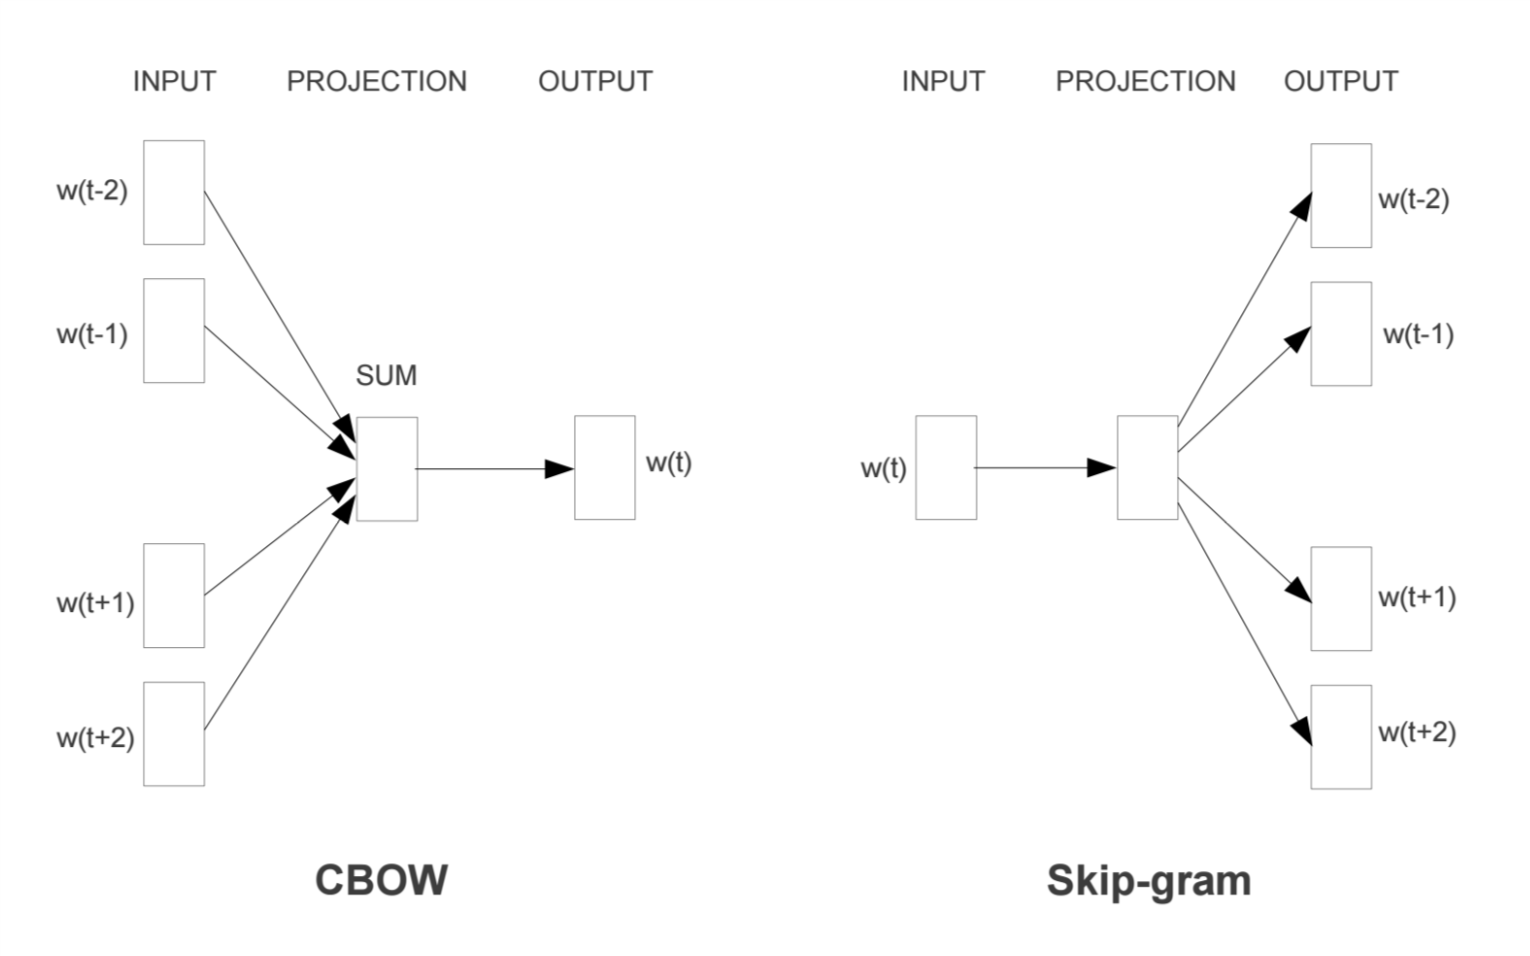
\includegraphics[width=0.85\linewidth]{images/word2vec}
	\caption{CBOW and Skip-gram architectures~\citep{mikolov2013efficient}}
	\label{fig:word2vec}
\end{figure}

Word2Vec has two architectures, namely Continuous Bags of Words (CBOW) and Skip-gram~\citep{mikolov2013efficient}, as illustrated in Figure~\ref{fig:word2vec}. In CBOW, the model learns to predict a word based on its neighboring words. Therefore, the input layer is represented with the bag-of-words. In contrast, Skip-gram architecture aims to predict the neighboring words based on a given word. The advantage of CBOW is that it can be used for training a huge amount of data, while Skipgram is best for capturing the average co-occurance from two words from the data.

Both architectures mainly aims to build language model, however, one does not need the whole trained model for having the word embedding representation. Instead, one only needs to extract the weight matrix used for converting words into vectors from the model. This weight matrix is the word embedding model that we use for transforming the words into dense vectors.

\section{Deep Learning}
Deep learning is a branch of machine learning that has multiple layers inside the model. Deep learning is able to extract implicit features in a high, abstract level~\citep{lecun2015deep}. Deep learning model has proved to produce robust performance in a variety of reserach, including computer vision and natural language processing.

Deep learning is basically a neural networks model with deeper hidden units. Neural networks model is based on how the neuron works inside human brain. Neurons with deep hidden units are then able to extract features in a abstract level~\citep{bengio2007scaling}. The deep learning structure consists of input layer, hidden layer, and output layer. The input layer is where the data being fed into the model, while output layer is the result of the model. The important layer here is the hidden layer in which a linear and/or non-linear functions are approximated in order to get the best predicted outputs.

Deep learning model has proved to give outstanding performances in supervised learning~\citep{Goodfellow-et-al-2016-Book}. A model with deeper layer will learn more implicit features out of the training data. There are a lot of deep learning architectures that have been proposed, one of which is the Recurrent Neural Networks~\citep{elman1990finding}. Each deep learning architecture is designed to fulfill specific computation needs.

\subsection{Recurrent Neural Networks}
Recurrent Neural Networks, shortened as RNN, is one of deep learning architectures designed for processing sequential data. There are some varieties of RNN, including the one proposed by~\cite{elman1990finding} and~\cite{jordan1986attractor}. Since it is designed for processing sequential data, it has a nature advantage for modeling the sequence labeling problem. Suppose that we have sequence of inputs, RNN will take each input in a time step $t$ to process it in a function. Figure~\ref{fig:simplernn} shows a general RNN.

\begin{figure}
	\centering
	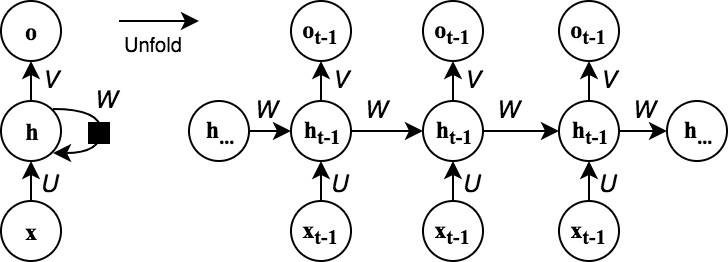
\includegraphics[width=0.80\linewidth]{images/RNNNew}
	\caption{A simple Recurrent Neural Networks (RNN). (left) folded RNN. (right) unfolded RNN}
	\label{fig:simplernn}
\end{figure}

The left picture illustrates the folded RNN model applied to all time steps. Note that the black rectangle represents one time step delay, meaning that that input is coming from the output of the previous time step. 

The right picture shows the unfolded RNN that is more intuitive since it visualizes the time steps. There are three layers in every time step t, which are input, hidden, and output layers. The input layer is for the input representations. In the hidden layer, it contains information from the input layer as well as those coming from hidden layers in the previous time steps. The output layer consists of the output of the model. These three layers are in a form of vectors. In every time step $t$, RNN has an input layer $ \mathbf{x_{t}} \in {\rm I\!R^{A}} $, hidden layer $ \mathbf{h_{t}} \in {\rm I\!R^{H}} $, and output layer $ \mathbf{o_{t}} \in {\rm I\!R^{B}} $. The values of $A$, $H$, and $B$ represent the length of the input vector, the number of unit in a hidden layer, and the length of the output vector, respectively. There are three parameters that will be trained, which are $U$, $V$, and $W.$ These parameters are the weight matrices for connecting two layers. $ U \in {\rm I\!R^{H \times A }}$ connects input layer with hidden layer (input-hidden), $ W \in {\rm I\!R^{H \times H}}$ connects hidden layer with the previous hidden layer (hidden-hidden), and $ V \in {\rm I\!R^{B \times H}}$ connects hidden layer with output layer (hidden-ouput). These parameters are time-distributed, meaning that they are shared across time steps. 

Every input layer $ \mathbf{x_{t}} $ is mapped into output layer $ \mathbf{o_{t}} $ in every time step $t$. In the middle of the process, the model calculates the hidden layer $ \mathbf{h_{t}} $ from two layers, $ \mathbf{x_{t}} $ and $ \mathbf{h_{t-1}} $. The output layer $ \mathbf{o_{t}} $ is then retrieved by performing a function to the hidden layer $\mathbf{h_{t}}$. The general equations for RNN are presented as follows:
\begin{equation}
\label{eq:rnnot}
\mathbf{o_{t}} = f2(V \cdot \mathbf{h_{t}} + \mathbf{c})
\end{equation}

\begin{equation}
\label{eq:rnnht}
\mathbf{h_{t}} = f1(U \cdot \mathbf{x_{t}} + W \cdot \mathbf{h_{t-1}} + \mathbf{b})
\end{equation}

Where $ \mathbf{h_{0}} = f1(U \cdot \mathbf{x_{0}}) $.

Note that there are two additional parameters to train, which are the bias vectors $\mathbf{b}$ and $\mathbf{c}$. In Equation~\ref{eq:rnnht}, the input $\mathbf{x_{t}}$ and $\mathbf{h_{t-1}}$ are weighted by matrices $U$ and $W$ respectively, added by a bias vector $\mathbf{b}$. The result is then inserted to an activation function $f1$ in order to produce hidden layer $\mathbf{h_{t}}$. In the Equation~\ref{eq:rnnot}, $\mathbf{h_{t}}$ is multiplied by the weight matrix $V$ and added by a bias vector $\mathbf{c}$ before being processed by the activation function $f2$ to produce $\mathbf{o_{t}}$. The examples of activation function $f1$ and $f2$ are tanh and softmax.

Based on this illustration, there are two main characteristics of RNN:
\begin{enumerate}
	\item It has a cycle in the graph for every time step. Hidden layer $\mathbf{h_{t-1}}$  will be one of the inputs for forming $\mathbf{h_{t}}$ .
	\item It has shared parameters across time steps.
\end{enumerate}

Figure~\ref{fig:fulrnn} illustrates a more complete RNN model on how it is being trained.

\begin{figure}
	\centering
	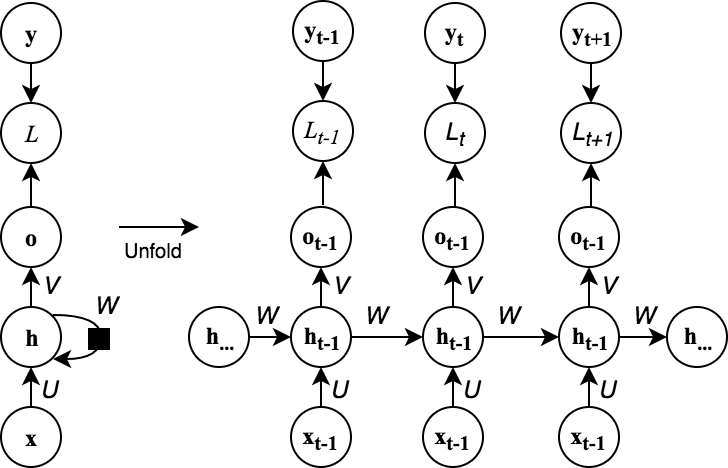
\includegraphics[width=0.80\linewidth]{images/RNNUnfoldNew}
	\caption{A Complete RNN on how it is being trained. (left) folded RNN. (right) unfolded RNN}
	\label{fig:fulrnn}
\end{figure}

The goal of training the model is to find the estimated values of parameters $W$, $U$, $V$, $\mathbf{b}$, and $\mathbf{c}$ which produce output $\mathbf{o_{t}}$ as close as the expected output $\mathbf{y_{t}}$ in the training data. 

The loss function $L$ measures the difference between the predicted output $\mathbf{o_{t}}$ and the expected output $\mathbf{y_{t}}$ in every time step t. The smaller the difference, the better the model. The machine thus has to minimize the result of loss function as small as possible. The parameters $W$, $U$, $V$, $\mathbf{b}$, and $\mathbf{c}$ are unknown in the beginning. At first, these parameters are initiated randomly. For every iteration, called epoch, the machine aims to learn the best values for each parameter.

The way to do so is by computing the gradient for each iteration. The idea behind computing the gradient values is to tell the model which parameter setting that brings it into smaller loss function result. By having this information, the machine then sets the better values for each parameter in the next iteration in order to reduce the loss function. From one iteration into another, the machine will find better parameter values to minimize the loss function. The learning method based on the gradient information is called optimization algorithm. Some optimization algorithms available are Adam~\citep{kingma2014adam}, and RMSProp~\citep{tieleman2012lecture}.

\subsection{Long Short-Term Memories}
Regular RNN has an issue called vanishing and exploding gradient problem. The RNN architecture repeatedly uses the same parameters for each time steps. Suppose that we use $W$ as the parameter for each time step between the hidden units. After $t$ time steps, the matrix would be multiplied $t$ times, hence it is the same as multiplying the hidden units with $W^{t}$~\citep{Goodfellow-et-al-2016-Book}. Assuming that $W$ has an eigen-decomposition $W = X \cdot diag(\lambda) \cdot X^{-1}$, $W^{t}$ is equal to:
\begin{equation}
W^{t} = (X \cdot diag(\lambda) \cdot X^{-1})^{t} = (X \cdot diag(\lambda)^{t} \cdot X^{-1})
\end{equation}

The eigenvalues $\lambda$ in $diag(\lambda)$ will either vanish if they are less than 1 in magnitude or explode if they are greater than 1 in magnitude. The gradient counted in each time step is aligned with the eigenvalues. Hence, the gradient may also vanish or explode. This is what we called as vanishing and exploding gradient problem. When the gradient vanishes, it is hard for the machine to find the direction to reduce the lost function. In the case of exploding gradient, the learning algorithm will become unstable.

To address this issue, there are solutions proposed such as simulated annealing and discrete error propagation~\citep{bengio1994learning}, time delays~\citep{lang1990time}, and hierarchical sequence compression~\citep{schmidhuber2007training}. Among these approaches, one of the most robust solutions is the Long Short Term Memories (LSTM)~\citep{hochreiter1997long}. 

The modification added in LSTM to address the issue is by using gates. It is basically RNN, but the nonlinear units in the hidden layer is replaced by the memory blocks. One nonlinear unit $tanh$ in RNN is replaced by more complex memory blocks in LSTM. Besides the hidden layer $\mathbf{h_{t}}$, LSTM also has $\mathbf{m_{t}}$ which is called memory cells.  The idea of LSTM is to learn when to forget or remember the memory from previous time steps through multiplicative gates. It thus prevents the vanishing and exploding gradient problem. For example, if the input gate is closed, then the memory will be unchanged.

Figure~\ref{fig:lstm} illustrates a one block memory in LSTM. There are three main gates, which are forget gate, input gate, and output gate. These gates are responsible to determine whether an information is added, kept, or deleted in a cell. Each gate has sigmoid layer and element-wise operations. The sigmoid layer converts the input into a probability between 0 and 1. This probability describes the gate behavior towards the input, whether to accept it (probability close to 1) or not (probability close to 0). 

\begin{figure}
	\centering
	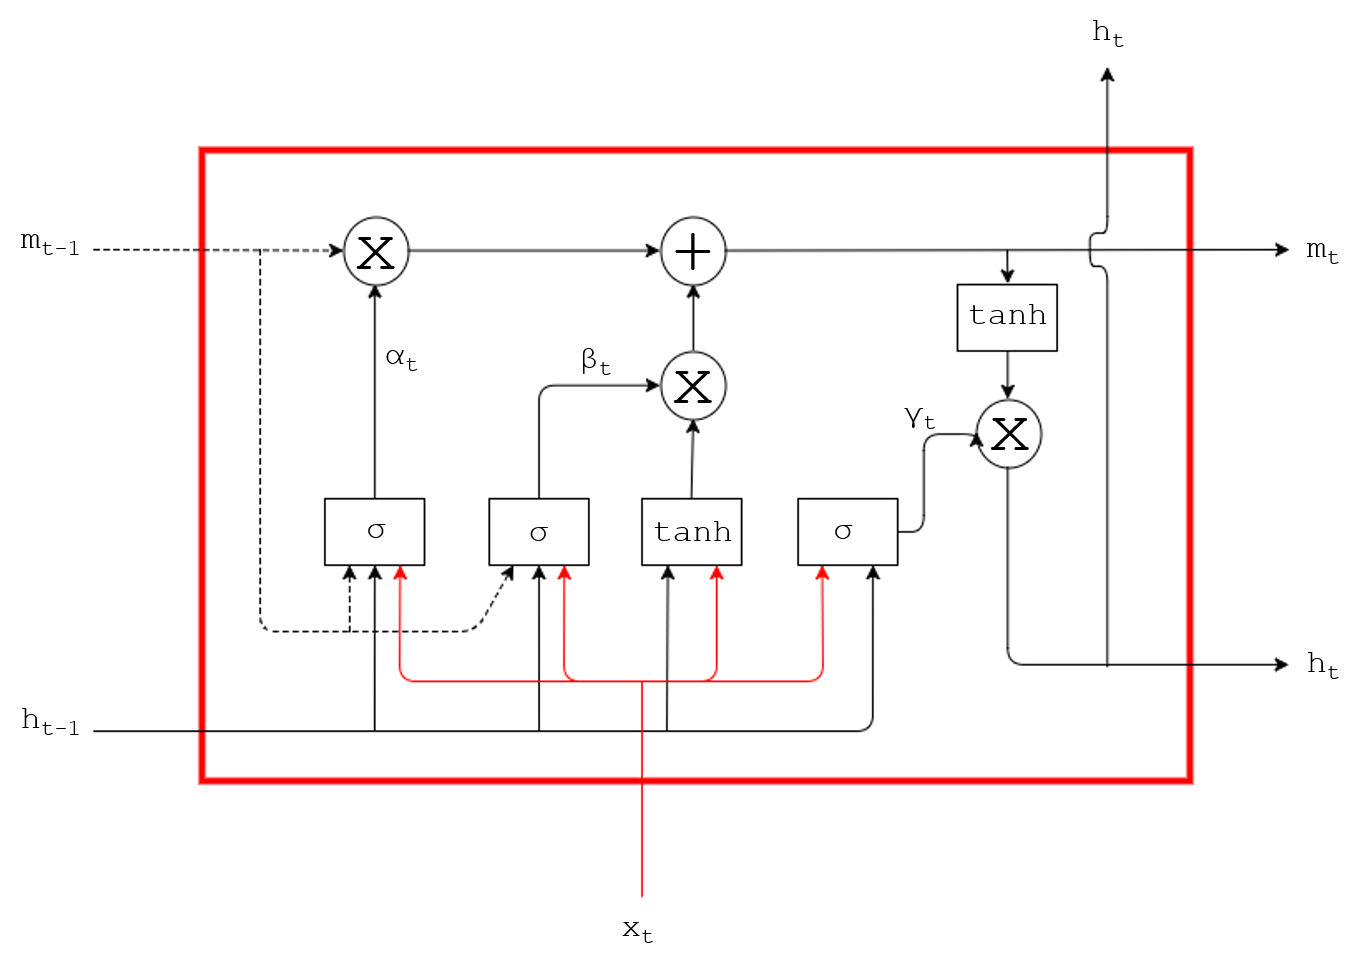
\includegraphics[width=1.0\linewidth]{images/lstm}
	\caption{One memory block in LSTM~\citep{skripsiwahid}}
	\label{fig:lstm}
\end{figure}

The equations of the sigmoid layers for each of the gates are explained as follows:
\begin{enumerate}
	\item \textit{Forget Gate}\\
	This gate is responsible to determine how much the information from the past should be kept in the memory. The equation of the forget gate is given as follows:
	\begin{equation}\label{eq:forget_lstm}
	\alpha_{t}=\sigma(W_{x\alpha}\cdot \mathbf{x_{t}}+W_{h\alpha}\cdot~\mathbf{h_{t-1}}+W_{m\alpha}\cdot~\mathbf{m_{t-1}})
	\end{equation}
	
	\item \textit{Input Gate}\\
	This gate is responsible to determine how much the current information x(t) should be kept in the memory. The equation of the input gate is given as follows:
	\begin{equation}\label{eq:input_lstm}
	\beta_{t}=\sigma(W_{x\beta}\cdot \mathbf{x_{t}}+W_{h\beta}\cdot~\mathbf{h_{t-1}}+W_{m\beta}\cdot~\mathbf{m_{t-1}})
	\end{equation}
	
	\item \textit{Output Gate}\\
	This gate is responsible to determine the output of a time step based on current cell state. The equation of the output gate is given as follows:
	\begin{equation}\label{eq:output_lstm}
	\gamma_{t}=\sigma(W_{x\gamma}\cdot \mathbf{x_{t}}+W_{h\gamma}\cdot~\mathbf{h_{t-1}}+W_{m\gamma}\cdot~\mathbf{m_{t-1}})
	\end{equation}
	
\end{enumerate}

In every time step $t$, the equations for computing cell state $\mathbf{m_{t}}$ and hidden layer $\mathbf{h_{t}}$ are presented as follows:
\begin{equation}\label{eq:mt}
\mathbf{m_{t}}=\alpha_{t} (\times) \mathbf{m_{t-1}} + \beta_{t} (\times) tanh(W_{xm} \cdot \mathbf{x_{t}} + W_{hm} \cdot \mathbf{h_{t-1}}))
\end{equation}
\begin{equation}\label{eq:ht}
\mathbf{h_{t}}=\gamma_{t} (\times) tanh(\mathbf{m_{t}})
\end{equation}

\section{Semantic Role Labeling}
Semantic role labeling (SRL) is a task in Natural Language Processing to assign semantic roles for each argument for each predicate in given input sentence~\citep{jurafsky2016speech}. In this section, the definition of semantic roles and the most commonly used annotation corpora for SRL are explained. In the end, the details on the semantic role labeling task are described.

\subsection{Semantic Roles}
Semantic roles are the representations that express the abstract role of the arguments of a predicate can take in the event~\citep{jurafsky2016speech}. When it comes to understanding natural language, one would want to understand the events and their participants of a given input sentence. In this case, the events refer to the predicate and the participants refer to the argument. Table~\ref{tab:examplesrl1} illustrates the connection between a predicate and its arguments.

\begin{table}
	\centering
	\caption{An example predicate and its arguments}
	\label{tab:examplesrl1}
	\begin{tabular}{|ccc|}
		\hline
		\underline{Andy} & \underline{eats} & \underline{fried chicken} \\
		\textsc{Argument} & \textsc{Predicate} & \textsc{Argument} \\
		\hline
	\end{tabular}
\end{table}

In this example, "eat" is the predicate with "Andy" and "fried chicken" as its argument. With this point of view, the predicate can be seen as the center of the sentence, followed by the arguments that depend on it.

Knowing the predicate and its arguments is not enough to understand the sentence since the roles of the arguments towards the predicate are unknown. In the previous example, it will be more meaningful to differentiate that "Andy" is the \textsc{Eater} and fried chicken is the \textsc{EatenThing}. \textsc{Eater} and \textsc{EatenThing} are the examples of semantic roles for the predicate "eat". These semantic roles could be used to identify the roles of the arguments regardless its position in the sentence. The previous example could be represented in two ways, as presented in Table~\ref{tab:examplesrl2}

\begin{table}
	\centering
	\caption{Examples of a predicate and its deep roles}
	\label{tab:examplesrl2}
	\begin{tabular}{|ccc|}
		\hline
		\underline{Andy} & \underline{eats} & \underline{fried chicken} \\
		\textsc{Eater} & \textsc{Predicate} & \textsc{EatenThing} \\
		\hline
		\underline{The fried chicken} & is \underline{eaten} & by \underline{Andy} \\
		\textsc{EatenThing} & \textsc{Predicate} & \textsc{Eater} \\
		\hline
	\end{tabular}
\end{table}

Both sentences represent the role of "Andy" and "fried chicken" as \textsc{Eater} and \textsc{EatenThing} respectively, regardless of their position in the sentence as a subject or object.

There are many ways to define such semantic roles. From the example above, the semantic roles are very specific for its predicate, known as deep roles~\citep{jurafsky2016speech}. \textsc{Eater} and \textsc{EatenThing} are the semantic roles for the predicate "eat", \textsc{Kicker} and \textsc{KickedThing} are the semantic roles for the predicate "kick", and so on. In order to further knowing more about the semantics of these arguments, the semantic roles could be generalized into more abstract roles. \textsc{Eater} and \textsc{Kicker} have something in common: they are volitional actors having direct causal responsibility for the predicate. Volitional means that the actors have the willing to decide on and commit to a particular action that they do. For this reason, thematic roles are introduced as a set of semantic roles designed to capture semantic commonality between \textsc{Eater} and \textsc{Kicker}~\citep{jurafsky2016speech}. With this in mind, \textsc{Eater} and \textsc{Kicker} can be represented as AGENT, which represents the abstract concept that is a volitional causer of an event (or predicate). On the other hand, \textsc{EatenThing} and \textsc{KickedThing} both represent the direct objects that are affected by the event. The thematic role for \textsc{EatenThing} and \textsc{KickedThing} is THEME.

Table~\ref{tab:examplesrl3} describes the thematic roles often used across computational papers~\citep{jurafsky2016speech}
\begin{table}
	\scriptsize
	\centering
	\caption{Examples of thematic roles~\citep{jurafsky2016speech}}
	\label{tab:examplesrl3}
	\begin{tabular}{lll}
		\hline
		\textbf{Thematic Role} & \textbf{Definition} & \textbf{Example} \\
		\hline
		AGENT & The volitional causer of an event & \underline{The waiter} spilled the soup \\
		EXPERIENCER & The experiencer of an event & \underline{John} has a headache \\
		FORCE & The non-volitional causer of the event & \underline{The wind} blows debris \\
		THEME & The participant directly affected by an event & Benjamin Franklin broke \underline{the ice} \\
		RESULT & The end product of an event & The city built \underline{a requlation-size baseball diamond} \\
		CONTENT & The content of a propositional event & Mona asked \underline{"Did you met Mary Ann?"} \\
		INSTRUMENT & An instrument used in an event & He stunned catfish with \underline{a shocking device} \\
		BENEFICIARY & The beneficiary of an event & Ann Callahan makes hotel reservations for \underline{her boss} \\
		SOURCE & The origin of the object of a transfer event & I flew in \underline{from Boston} \\
		GOAL & The destination of an object of a transfer event & I drove \underline{to Portland} \\
		\hline
	\end{tabular}

\end{table}

AGENT and EXPERIENCER represent the volitonal causer of an event and the experiencer of an event, respectively. While AGENT is volitional, the non-volitional causer of an event is called FORCE. Furthermore, THEME and RESULT are the participant directly affected by an event and the end product of an event, respectively. BENEFICIARY represents the beneficiary of an event. CONTENT describes the content of a propositional event. An instrument used in an event is called INSTRUMENT. For location, there are SOURCE and GOAL which represent the origin and the destination of an object of a transfer event.


\subsection{Annotation Corpus}
There are available annotated corpus for SRL consisting of sentences labeled with semantic roles. Researchers are using these annotated corpus for building supervised machine learning model for SRL. The two most commonly used annotation corpus for SRL are Proposition Bank and FrameNet.

\subsubsection{Proposition Bank}
Proposition Bank~\citep{kingsbury2002treebank}, shortened as PropBank, is a corpus in which sentences are annotated with semantic roles. PropBank corpus is available for many languages, such as English, Chinese, Hindi, Arabic, Finnish, and Portuguese. The main approach used for its semantic roles grouping is based on proto-roles and verb-specific semantic roles. Every verb sense has its set of semantic roles with argument numbers rather than names, for example: Arg0, Arg1. Arg2, etc. Usually, Arg0 represents PROTO-AGENT while Arg1 represents PROTO-PATIENT. Other argument number representations may vary based on each verb sense.

Both PROTO-AGENT and PROTO-PATIENT are generalized roles that describe roughly agent-like and roughly patient-like meanings, respectively~\citep{jurafsky2016speech}. Both roles are defined by heuristic features that describe more agent-like or more patient-like meanings. For instance, when the argument has more agent-like properties (causing an event, causing a change of state of other participant, being volitionally involved in the event) the likelihood that the argument can be labeled as PROTO-AGENT will be greater. On the other hand, the more an argument has patient-like properties (causally affected by another participant, undergoing change of state), the bigger the likelihood that the argument to be labeled as PROTO-PATIENT. 

The PropBank entries are called frame files. One example of the frame files for one sense of verb eat is presented as follows.
\\
\fbox{%
	\parbox{1.0\linewidth}{%
		\textbf{Frame File:}\\
		\textit{Eat.01}\\
		Arg0: Eater\\
		Arg1: Things Eaten\\
		Arg2: Instrument used\\
		\\
		\textit{Example:}\\
		Ex1: [Arg0 Andy] eats [Arg1 fried chicken] [Arg2 with spoon]\\
		Ex2: [Arg1 That fried chicken] is eaten by [Arg0 Andy] [Arg2 with spoon]
	}%
}
\\

For verb sense Eat.01, Arg0 acts as the Eater (PROTO-AGENT), and Arg1 represents the Things Eaten (PROTO-PATIENT). As we can see from the example above, we can infer the commonality between examples Ex1 and Ex2 regardless its structure, be it in a passive or active voice. In both examples, Andy is the Eater and fried chicken is the Things Eaten. In this frame file, there is also another argument, Arg2, that represents the instrument used by the Eater. In example Ex1 and Ex2, the instrument is spoon.

Other non-numbered arguments are available in PropBank, the so-called ArgMs, representing modifiers that could be used across frame files. Some examples of ArgMS include:
\\
\fbox{%
	\parbox{1.0\linewidth}{%
		TMP: When?\\
		LOC: Where?\\
		DIR: Where to/from?\\
	}%
}
\\

The next annotation corpus is called FrameNet which has different approach on how to group the set of semantic roles. Instead of using verb-specific, it uses frame-specific grouping.

\subsubsection{FrameNet}
FrameNet~\citep{baker1998berkeley} is an annotation corpus for semantic roles that are specific to a frame. In PropBank, the semantic roles are defined based on each sense of a verb. In contrast, a frame in FrameNet could include more than one predicate (verbs or nouns) that have the same background context. Each frame consists of two elements: 1.) A set of semantic roles related to this frame, and 2.) A set of predicates using the respective semantic roles.

One example is a frame called $\mathbf{change\_position\_on\_a\_scale}$~\citep{jurafsky2016speech} defined as:
\\
\fbox{%
	\parbox{1.0\linewidth}{%
		\texttt{This frame consists of words that indicate the change of an Item's position on a scale (the Attribute) from a starting point (Initial value) to an end point (Final value).} \\
	}%
}
\\

The set of semantic roles for a frame is divided into two roles: Core roles and Non-Core Roles. Core Roles are specific to a frame while Non-Core Roles are more general across frames (like ArgMs in PropBank). The set of semantic roles of the frame $\mathbf{change\_position\_on\_a\_scale}$ is explained as follows.
\\
\fbox{%
	\parbox{1.0\linewidth}{%
		\textbf{Core Roles}\\
		ITEM: The entity that has a position on the scale.\\
		ATTRIBUTE: The ATTRIBUTE is a scalar property that the ITEM possesses\\
		DIFFERENCE: The distance by which an ITEM changes its position on the scale. FINAL STATE: A description that presents the ITEM's state after the change in the ATTRIBUTE's value as an independent predication.\\
		FINAL VALUE: The position on the scale where the ITEM ends up. \\
		INITIAL STATE: A description that presents the ITEM's state before the change in the ATTRIBUTE's value as an independent predication.\\
		INITIAL VALUE:The initial position on the scale from which the ITEM moves away. \\
		VALUE RANGE: A portion of the scale, typically identified by its end points, along which the values of the ATTRIBUTE fluctuate. \\
		\\
		\textbf{Non-Core Roles}\\
		DURATION: The length of time over which the change takes place.\\
		SPEED: 	The rate of change of the VALUE.\\
	}%
}
\\

For instance, the possible predicates of the frame change position on a scale are: \textit{rose, increase, fell}.

The example of semantic roles of the frame $\mathbf{change\_position\_on\_a\_scale}$ can be seen as follows:

[ITEM Oil] rose [ATTRIBUTE in price] [DIFFERENCE by 2\%]. 

[ITEM It] has increased [FINAL STATE to having them 1 day a month]. 

[ITEM Microsoft shares] fell [FINAL VALUE to 7 5/8]. 

[ITEM Colon cancer incidence] fell [DIFFERENCE by 50\%] [GROUP among men]

a steady increase [INITIAL VALUE from 9.5] [FINAL VALUE to 14.3] [ITEM in dividends]

a [DIFFERENCE 5\%] [ITEM dividend] increase... 

As we can see from the examples above, \textit{rose}, \textit{fell}, and \textit{increase} have the same set of semantic roles under the frame $\mathbf{change\_position\_on\_a\_scale}$. Instead of defining the semantic roles for each verb sense one by one, FrameNet groups predicates (not limited to verbs) that have same semantic roles as one frame.
%\subsection{Problem Definitions}
%Semantic Role Labeling (SRL) is one of Natural Language Processing task which aims to automatically assign semantic roles for each constituent (argument) for each predicate in a sentence~\citep{jurafsky2016speech}. Current approach to solve this task is by using supervised machine learning. Given a labeled data, the machine learns from it and builds a generalization model. Researches often used PropBank or FrameNet corpus as the sources of annotated data. In this section, we describe the approaches to define the problem of SRL task, followed by the common features used for building supervised model for SRL.
%
%There are two ways to see SRL problem, either as Classification or Sequence Labeling problem. Classification approach assigns semantic roles for each word independently. Meanwhile, Sequence Labeling approach traverses from assigning semantic role for the first word until the last one in a sentence sequentially. In Sequence Labeing, the next label (semantic role) prediction of time step t is dependent to labels predicted on previous time steps (1..t-1).
%
%In classification approach approach, suppose that we have an input of \textit{n} words $w = (w_{1}, w_{2}, ..., w_{n})$. Each vector $w_{i}$ is classified into a label $y_{i}$ that represents the semantic role. The probabilities of the label in each time step $i$ is described as follows.
%\begin{equation}
%P(y_{i}|w_{i})
%\end{equation}
%
%In sequence labeling approach, suppose that we have an input of \textit{n} words $w = (w_{1}, w_{2}, ..., w_{n})$, the goal is to find the best label sequence $y = (y_{1}, y_{2}, ..., y_{n})$, with $y_{i}$ representing the semantic roles. The probabilities of the label in each time step $i$ is described as follows.
%\begin{equation}
%P(y_{i}|w_{i-l}, ..., w_{i+l},y_{i-l}, ..., y_{i+l})
%\end{equation}
%
%whereby \textit{l} is a small number. 

\subsection{Common Features for SRL}
The first set of features for SRL is proposed by~\cite{gildea2002automatic}. They are the first ones who used supervised machine learning approach to solve SRL. Over the years, many research proposed new set of features to improve the result. The common features used for solving SRL task are presented as follows~\citep{jurafsky2016speech}.
\begin{enumerate}
	\item The predicate.\\
	Usually in a form of verb.
	\item The phrase type of the constituent.\\
	NP, PP, etc
	\item The headword of the constituent.\\
	Example: The black \textit{bird}.
	\item The headword part of speech of the constituent. \\
	Example: The black \textit{bird}. POS of \textit{bird} is Noun.
	\item The path of the parse tree from constituent to predicate. \\
	This is to represent the grammatical relationships between the constituent and the predicate.
	Example: NP-S-VP-VBD
	\item The voice of the clause, active or passive.\\
	Example: I eat chicken rice (active), Chicken rice is eaten by me (passive).
	\item The binary linear position of the constituent from the predicate.\\
	Could be before or after the predicate.
	\item The subcategorization of the predicate\\
	Set of arguments that appear in the verb phrase VP.
	Example: NP and PP in 'VP -> VBD NP PP'
	\item The named entity type of the constituent\\
	Example: Organization, Person, Location
	\item The first and last words of the constituent.
\end{enumerate}

There are also other additional features that could be used for SRL, such as sets of n-grams inside the constituent. Another variation is to use dependency parser instead of syntactic parser for extracting features.

\subsection{Historical Perspectives}
SRL can be seen as either a classification or sequence labeling problem. The earlier research on SRL was conducted with the classification approach, meaning that each argument is being predicted independently from the others. Those research focused on how to extract meaningful features out of syntactic parsers~\citep{gildea2002automatic, gildea2002necessity, pradhan2005semantic}, such as the path to predicate and constituent type. This syntactic information plays a pivotal role in solving SRL problem~\citep{punyakanok2008importance} as it addresses SRL's long distance dependency~\citep{zhou2015end}. Thus, traditional SRL system heavily depends on the quality of the parsers. The analysis done by~\cite{pradhan2005semantic} shows that most errors of the SRL system were caused by the parser's error. In addition, those parsers are costly to build, since it needs linguistic experts to annotate the data. If we want to create an SRL system on another language, one should build a new parser all over again for it~\citep{zhou2015end}.

In order to minimize the number of hand-crafted features, ~\cite{collobert2011natural} utilized deep learning for solving NLP tasks including Part-of-Speech Tagging (POS), Chunking (CHUNK), Named Entity Recognition (NER), and Semantic Role Labeling (SRL) with classification approach. The research aimed to prevent using any task-specific feature in order to achieve state-of-the-art performance. The word embedding is used as the main feature across tasks, combined with Convolutional Neural Networks (CNN) architecture to train the model. They achieve promising results for the POS Tagging, Chunking and NER, while for SRL features from the parsers are still needed to achieve competitive results.

Different from the previous works,~\cite{zhou2015end} view SRL as a sequence labeling problem in which the arguments are labeled sequentially instead of independently. They proposed an end-to-end learning of SRL using Deep Bi-Directional Long Short-Term Memories (DB-LSTM), with word embedding as the main feature. Their analysis suggests that the DB-LSTM model implicitly extracts the syntactic information over the sentences and thus, syntactic parser is not needed. The research result outperforms the previous state-of-the-art traditional SRL systems as it achieves F1 score of 81,07\%. The research also shows that the performance of the sequence labeling approach using DB-LSTM is better than the classification approach using CNN, since the DB-LSTM can extract syntactic information implicitly.

%While many of the previous works studied SRL on formal language, our research aims to explore SRL on conversational language, which is still under-resourced. We thus introduce a new set of semantic roles for this language type. Furthermore, we propose a new architecture named Context-Aware Bi-Directional Long Short-Term Memories, designed with attention mechanism in order to capture context information of the sentence at a higher level.

% OR THIS ONE, ELLABORATE BOTH %
%Previous research have found useful to use RNN for NLP task Semantic Role Labeling (SRL). Before we discuss about the use of RNN on SRL, we describe the historical perspective of solving SRL with supervised machine learning. We divide the historical perspective based on SRL systems without and with deep learning.
%
%The non-deep learning approach uses specific hand-crafted features for SRL, which mainly depend on syntactic or dependency parser as explained in section 2.XX. It started from Gildea et. Al (2002) who firstly build supervised machine learning model for SRL. The goal of the research was to create the first shallow semantic role parser which is not domain specific, since at that time all the semantic roles research were too domain specific. The features used are extracted from the syntactic tree Collins Parser (XX, 1997), such as Phrase Type, Parse tree path, voice, and head word. Then the predicate of a sentence is also added as a feature. The research used semantic role annotation based on FrameNet. The algorithm used was statistical classifier with backoff approach. The result is 65\% precision and 61\% recall.
%
%Then, Gildea et al (2002) continues the research to quantify the effect of parser accuracy on SRL system’s performance. The research also examines whether a flatter “chunked” representation (which is less costly) of the input can be as effective as syntactic tree parser. The data used is from PropBank dataset, since it is from Wall Street Journal corpus that has a gold-standard syntactic parse trees for the entire dataset from the Penn Treebank Project. The finding shows that the parser accuracy affects the SRL system, since it is seen that the system with gold-standard parse tree impacts directly to build a better SRL system. Hence, the syntactic parser is an integral intermediary model to build a robust SRL system. If the parser is not good, one would not get a good SRL system.
%
%Surdeanu et al (2003) proposed a new set of features for SRL system, such as POS Tag of Head Word, POS Tag of content word, and Named Entity Class of Content Word. They use inductive learning through decision trees C5 for the algorithm.
%
%Xue et al (2004) aims to explore more information extracted from the parse tree in order to propose new set of features crafted to improve SRL. In their research, there are three steps for the model, pruning, argument identification, and argument classification. Pruning filters out constituents that are clearly not semantic arguments to the predicate. Argument identification classifies candidates as either semantic arguments or non arguments. Argument classification then runs a multi-category classifier to classify the constituents with semantic roles. The features proposed for the argument classification are syntactic frame, lexicalized constituent type, lexicalized head word, and the head of Preposition Phrase parent.
%
%Since the source of SRL system errors mostly based on syntactic parser’s error, Pradhan et al (2005) combines features from different syntactic parsers (Charniak parser and Collins Parser). The idea of combining two parser is that they train separate SRL systems for each tree parser. The role output from these two systems is used as additional features in a SRL system using flat syntactic view. They then use SVM classifier to train SRL based on PropBank data.
%
%Aside from using syntactic parse tree like Charniak or Collins parser, one can build SRL system by extracting features from dependency parser. Some of the features extracted are word property, syntactic connection, semantic connection, and dependency path.
%
%The drawbacks of using the non-deep learning approach are 1.) building syntactic or dependency parsers is costly, 2.) the SRL system hardly depends on the robustness of the parsers. Building tree parsers is costly because it is language-dependent and it needs experts in each language to create it. When we move to another language, we have to build these parsers for the new language from scratch. Not to mention a new problem arises when such parsers are not robust, hence creating error propagation in our SRL system. The analysis in Pradhan et al., (2005) says that the major source of errors in SRL system comes from the errors of the syntactic parsers from which we extract the features.
%
%To address this issue, Collobert et al. (20XX) firstly introduced the use of deep learning for SRL and other core NLP tasks such as POS Tagging and Chunking. They use Convolutional Neural Network (CNN) with no task-specific features for the system. For example, in non-deep learning approach, we use POS Tagging features for Chunking, and we use both of which as the features for SRL. Instead, the main feature used in this research is word embedding. As explained in the previous section, word embedding model converts words to vectors. The word vectors then are fed into CNN architecture. However, though the model achieved state-of-the-art performances for POS Tagging and Chungking, that is not the case for SRL. For SRL, it is still needed to use features from the tree parser to achieve robust performance.
%
%Zhou et al., (2015) proposed new architecture for the SRL system. Instead of seeing the SRL as a classification problem like the previous research including Collobert’s, Zhou considers SRL as the sequence labeling problem. Hence, the suitable architecture for such problem is Recurrent Neural Networks (RNN). In their research, a more specific RNN architecture is used, which is Long Short Term Memories (LSTM) in order to prevent the vanishing and exploding gradient problem in RNN. They used the deep bi-directional LSTM. The “deep” is for extracting more hidden features and the “bi-directional” is for extracting information from the past and future. On top of the LSTM architecture, they used Conditional Random Field (CRF) for the output layer. For the word representation, they also used word embedding as one of the main features, along with predicate and context predicate. Our research is mainly inspired by this research.

% PUNYA WAHID %

%\section{Deep Learning}
%\textit{Deep Learning}, atau disebut juga \textit{deep structured learning, hierarchical learning,} dan \textit{deep machine learning} merupakan salah satu cabang dalam \textit{machine learning} yang model komputasinya terdiri dari beberapa layer. \textit{Deep learning} mampu mempelajari dan mengekstrak representasi data/fitur secara otomatis pada abtraksi tingkat tinggi \citep{lecun2015deep}. Model tersebut memberikan hasil yang sangat baik dalam penelitan di berbagai bidang seperti \textit{speech recognition}, \textit{object detection}, \textit{sequence labeling} dan lain sebagainya.  
%
%Struktur pembelajaran pada \textit{deep learning} berbentuk hierarki karena termotivasi dari bagaimana neokorteks pada otak maunusia bekerja secara mendalam. Neokorteks tersebut melakukan proses pemelajaran berlayer dan secara otomatis mampu mengketrak fitur dan melakukan abstraksi dari \textit{resource} yang diberikan \citep{bengio2007scaling}. Struktur tersebut terdiri atas \textit{input layer}, \textit{hidden layer} dan \textit{output layer}. \textit{Input layer} memiliki fungsi sebagai tempat masuknya data yang akan dipelajari oleh model. \textit{Hidden layer} melakukan aproksimasi fungsi untuk mendapatkan target dari data \textit{training} yang diberikan. Disebut \textit{hidden layer} karena pada layer ini, \textit{output} tidak bisa kita lihat \citep{Goodfellow-et-al-2016-Book}. \textit{Hidden layer} inilah yang menjadi \textit{key role} dalam \textit{deep learning}. Sedangkan \textit{output layer} merupakan layer untuk mengembalikan target yang diinginkan.
%
%\textit{Deep learning} ini mampu memberikan model yanng memiliki performa sangat baik dalam \textit{supervised learning} \citep{Goodfellow-et-al-2016-Book}. Dengan menambahkan lebih banyak layer dan unit di dalam layer, \textit{deep network} dapat merepresentasikan fungsi dengan kompleksitas yang tinggi. Secara umum, \textit{deep learning} memetakan \textit{input vector} ke \textit{output vector}. Walaupun hal ini mudah dilakukan oleh manusia secar manual, namun untuk \textit{dataset} yang sangat besar, tentu hal ini tidak mungkin dilakukan. Ada banyak macam model \textit{Deep Learning} yang sesuai dengan kebutuhan komputasi, seperti \textit{Deep Belief Network} \citep{hinton2006fast}, \textit{Recurrent Neural Networks} \citep{elman1990finding}, \textit{Long Short Term Memory} \citep{hochreiter1997long}, \textit{Restricted Boltzman Machine} \citep{pennington2014glove} dan lain sebagainya. 

%\section{Recurrent Neural Networks}\label{sec:rnns}
%
%\textit{Recurrent neural networks} (RNNs) merupakan merupakan salah satu arsitektur \textit{Deep Learning} yang memiliki koneksi siklik \citep{graves2012neural}. RNNs memiliki \textit{neuron} yang terkoneksi dengan \textit{neuron} lain sehingga membentuk \textit{loop} umpan balik (\cite{haykin2009neural}), tidak seperti \textit{feedforward neural network} (FNNs) dimana aliran informasi hanya berjalan searah. RNNs memungkinkan \iob~yang dihasilkan akan menjadi \ioa~untuk menghasilkan \iob~yang lain. Hal ini menyebabkan perilaku RNNs tidak hanya bergantung pada \ioa~saat ini saja, namun juga bergantung pada \iob~sebelumya. Oleh karena itu, RNNs memiliki kemampuan yang sangat bagus sebagai model dalam permasalahan \textit{sequence data} dibandingkan dengan FNNs. RNNs sendiri memiliki kemampuan yang sangat bagus dalam beberapa \textit{task} terkait \textit{sequence data}, seperti \textit{language model} (\cite{mikolov2010recurrent}) dan \textit{speech recognition} (\cite{graves2013speech}).
%
%Dibandingkan dengan FNNs, RNNs memiliki beberapa kelebihan \citep{mikolov2010recurrent}, yaitu:
%\begin{enumerate}
%	\item Pada RNNs, kata-kata sebelumnya direpresentasikan dengan \textit{recurrent connections}, sehingga RNNs dapat menyimpan informasi kata sebelumnya dalam jumlah tak hingga. FNNs tidak bisa secara alami memodelkan hubungan kontekstual antara sebuah kata dengan kata-kata pada posisi sebelumnya dan representasi kata sebelumnya berupa konteks dari $ n-1 $ kata. Oleh karena itu, FNNs terbatas dalam penyimpanan informasi kata sebelumnya terbatas seperti pada model \textit{n-gram}.
%	\item RNNs dapat melakukan kompresi keseluruhan riwayat kata menjadi ruang dimensi yang lebih kecil, sedangkan FNNs melakukan kompresi/proyeksi hanya dengan sebuah kata saja.
%\end{enumerate}


%!TEX root = skripsi.tex
%-----------------------------------------------------------------------------%
\chapter{\babTiga}\label{bab:tiga}
%-----------------------------------------------------------------------------%
%-----------------------------------------------------------------------------%
% Ide, model matematik, rumus, fitur, jangan m=ngomongin teknologi (java, keras, dll), word2vec boleh %
Pada bab ini \saya~akan menjelaskan metodologi penelitian yang \saya~gunakan. Metodologi penelitian yang dilakukan meliputi tahap pengumpulan data, pra-pemrosesan data, pelabelan data, pengembangan model, eksperimen dan evaluasi.

\section{Gambaran Umum Pengembangan Metodologi}
Penelitian ini bertujuan untuk membuat sebuah model yang mampu memberikan label entitas kesehatan pada suatu dokumen. Seperti yang telah dijelaskan pada bab sebelumnya, terdapat banyak entitas kesehatan yang dapat digunakan sebagai target pelabelan. Oleh karena itu, untuk mempermudah penelitian ini \saya~menggunakan entitas-entitas yang diusulkan oleh \cite{skripsiKakRadit} dalam penelitiannya,  nama penyakit (\textit{\disease}), gejala penyakit (\textit{\symptom}), obat (\textit{\drug}) dan langkah penyembuhan (\textit{\treatment}).

Penelitian ini menggunakan dua buah korpus, yaitu korpus dari data dokumen teks kesehatan yang digunakan \cite{skripsiKakRadit} dan dokumen teks hasil pengumpulan yang dilakukan oleh \saya~pada situs kesehatan \textit{online}. Setelah itu \saya~melakukan pra-pemrosesan pada kedua data sebelum melakukan tahap selanjutnya. Untuk dokumen hasil pengumpulan dari forum, \saya~memberi label kesehatan secara manual dengan ketentuan pelabelan pada penelitian \cite{skripsiKakRadit}

Setelah tahap pengusulan model, terdapat 2 eksperimen yang \saya~lakukan, yaitu eksperimen untuk mendapatkan fitur diskriminatif yang mampu membuat model memiliki akurasi terbaik dan eksperimen untuk mendapatkan arsitektur RNNs yang membuat model menghasilkan akurasi tertinggi. Pada eksperimen pertama, \saya~mencoba beberapa fitur, seperti fitur yang diusulkan oleh \cite{skripsiKakRadit} (fitur \textit{its own word}, frasa, kamus (\textit{symptom}, \textit{disease}, \textit{treatment} dan \textit{drug}), kata pertama sebelum, dan fitur kata setelah. Pada eksperimen kedua, \saya~mencoba dua arsitektur RNNs, yaitu RNNs yang setiap \textit{input} digabung terlebih dahulu dengan meng-\textit{append} semua vektor fitur. Sedangkan RNNs yang kedua yaitu RNNs yang setiap kelompok fitur menjadi \textit{input} bagi masing-masing LSTMs, baru kemudian \textit{output} dari layer tersebut digabung.

Setelah melakukan eksperimen, \saya~melakukan evaluasi dari hasil yang didapatkan dengan menghitung nilai \textit{precission}, \textit{recall} dan \textit{F-measure} dari masing-masing entitas secara keseluruhan. Untuk mendapatkan rata-rata akurasi dari setiap eksperimen, \saya~melakukan \textit{10-fold cross validation} dengan cara membagi semua data menjadi 10 bagian, 9 bagian menjadi data \textit{training} dan 1 \textit{bagian} menjadi data \textit{testing}. Proses tersebut diulang sebanyak sepuluh kali sehingga masing-masing bagian data menjadi data \textit{testing}.
\begin{figure}
  \centering
  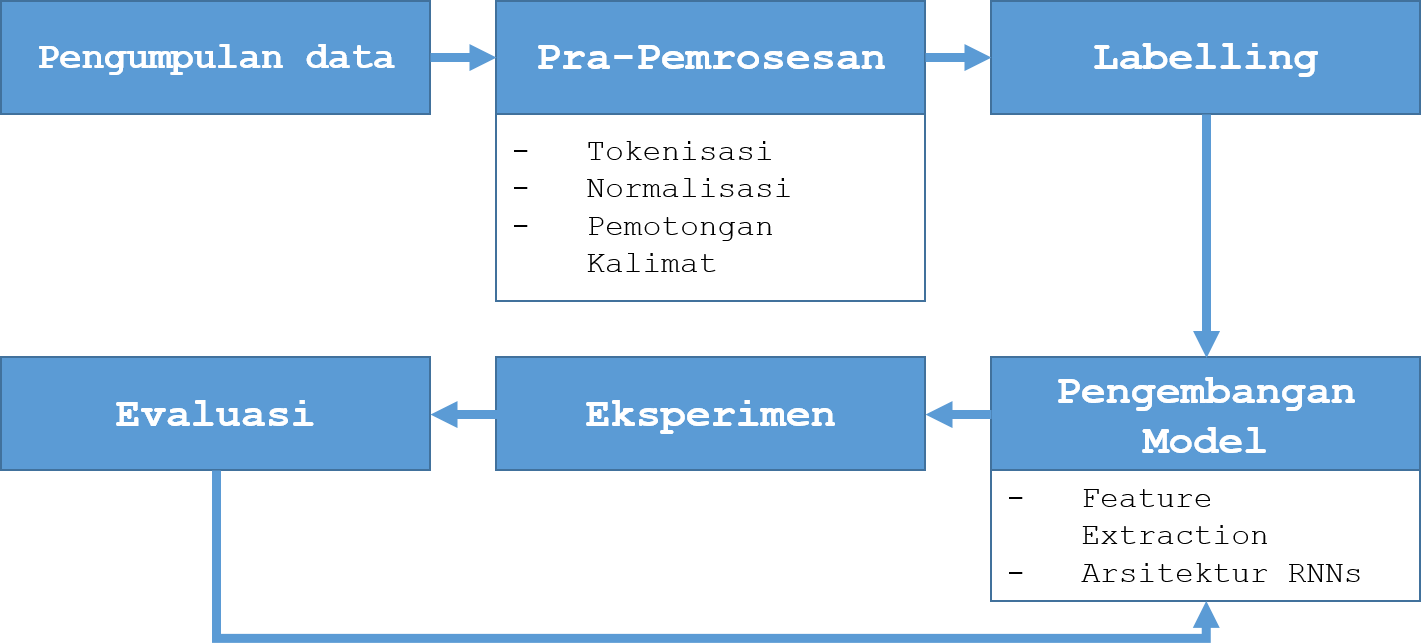
\includegraphics[width=\linewidth]{images/arsitektur}
  \caption{Diagram Gambaran Umum Metodologi yang Dilakukan}
  \label{fig:metodologi_penelitian}
\end{figure}

\section{Pengumpulan Data}
Pengumpulan data dilakukan dengan tujuan untuk mendapatkan data \textit{training} dan \textit{testing} yang akan digunakan sebagai \textit{resource} dalam melakukan \textit{training} dan evaluasi model \mer. Data yang dimaksud merupakan teks dari forum kesehatan \textit{online} dari berbagai sumber. Pada penelitian ini, \saya~menggunakan data penelitian \cite{skripsiKakRadit} dan data yang \saya~dapatkan dari hasil \textit{crawling} di forum kesehatan \textit{online}. Data yang \cite{skripsiKakRadit} diambil dari beberapa situs forum kesehatan \textit{online} dan sedangkan data yang \saya~unduh bersumber dari forum kesehatan \textit{online}.

\section{Pra-Pemrosesan}
Pra-pemrosesan dilakukan dengan tujuan supaya teks yang diberikan mampu dibaca oleh sistem \mer. Dalam tahap ini, ada tiga pekerjaan utama yang perlu dilakukan, yaitu:

\subsection{Pembersihan data}
Langkah ini dilakukan dengan tujuan untuk mempermudah proses POS \textit{tagging}. Selain itu, terdapat beberapa token yang berbeda sintaks namun memiliki jenis kata yang sama, misalnya token \textit{email}. Model hanya perlu tahu token tersebut merupakan email, tidak peduli pemilik email tersebut. Berikut merupakan beberapa langkah yang \saya~lakukan:
	
\begin{enumerate}
	\item menghapus karakter yang bukan merupakan karakter ASCII,
	\item mengganti token url menjadi kata "url", misalnya token tautan (\textit{www.alodokter.com/asma/pengobatan}) diganti menjadi token "url",
	\item mengganti token \textit{email} menjadi kata "email", misalnya sebuah alamat \textit{email} (\textit{wahid@domain.com}) diganti menjadi token "email",
	\item mengganti karakter "\_" menjadi token "underscore",
	\item mengganti karakter "\&" menjadi token "dan",
	\item mengganti karakter "\textless" dan "\textgreater" menjadi token "kurang dari" dan "lebih dari" dan
	\item mengganti karakter "/" menjadi token "atau".
\end{enumerate}
Pada langkah ini, \saya~tidak menghapus karakter tanda baca karena karakter tersebut memiliki fungsi pada sistem POS \textit{tagging} yang \saya~gunakan. Gambar \ref{fig:pembersihandata} merupakan contoh pembersihan data pada sebuah teks.
\begin{figure}
	\centering
	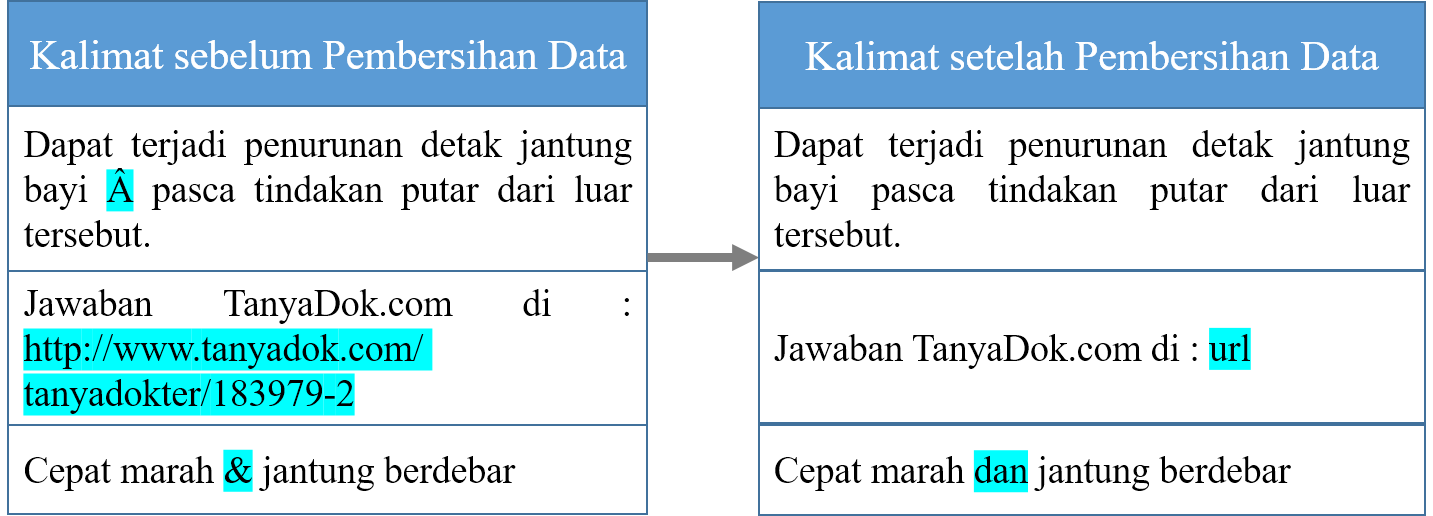
\includegraphics[width=\linewidth]{images/pembersihandata}
	\caption{Ilustrasi Pembersihan Data pada Kalimat}
	\label{fig:pembersihandata}
\end{figure}

	
\subsection{Tokenisasi}
Tokenisasi dilakukan untuk mendapatkan token yang paling tepat sebagai sebuah kata. Hal ini perlu dilakukan untuk menghindari beberapa kelompok token berbeda yang tergabung. Karakter abjad dengan karakter angka atau karakter abjad dengan karakter tanda baca dipisahkan berdasarkan kelompoknya. Misalnya token "pusing2" diubah menjadi "pusing 2". Pada tahap ini, \saya~melakukan pemisahan terhadap beberapa kelompok token, yaitu:
\begin{enumerate}
	\item <alfabet><numerik> menjadi <alfabet><spasi><numerik>
	\item <numerik><alfabet> menjadi <numerik><spasi><alfabet>
	\item <alfanumerik><non-alfanumerik> menjadi <alfanumerik><spasi><non-alfanumerik>
	\item <non-alfanumerik><alfanumerik> menjadi <non-alfanumerik><spasi><alfanumerik>
\end{enumerate}

Gambar \ref{fig:tokenisasi} berikut merupakan contoh tokenisasi pada sebuah teks.
\begin{figure}
	\centering
	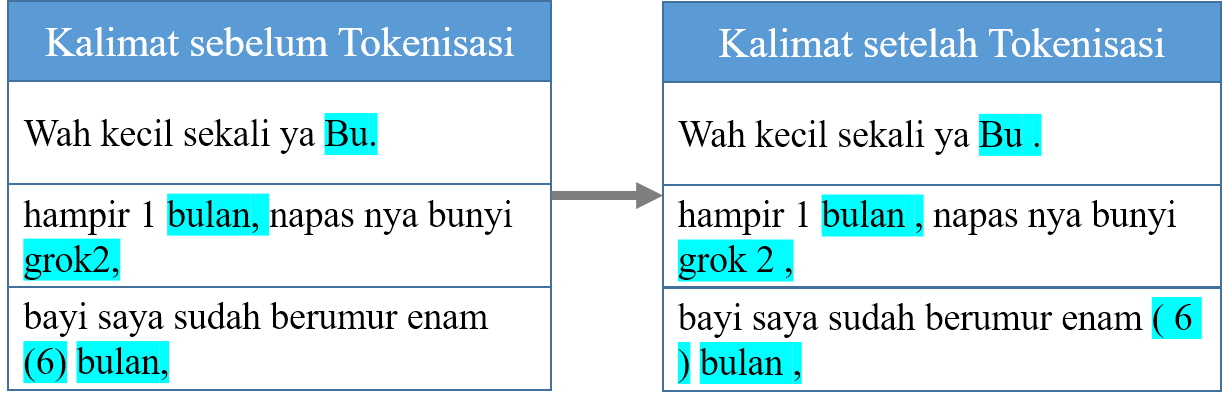
\includegraphics[width=\linewidth]{images/tokenisasi}
	\caption{Ilustrasi Tokenisasi pada Kalimat}
	\label{fig:tokenisasi}
\end{figure}

	
\subsection{Pemotongan kalimat}
Untuk menghindari jumlah token yang timpang dalam kalimat yang berbeda dan data yang \textit{sparse}, \saya~melakukan pemotongan kata dengan langkah-langkah sebagai berikut:
\begin{enumerate}
	\item memisahkan kalimat berdasarkan tanda baca (.!?,),
	\item apabila suatu kalimat memiliki jumlah kata yang sedikit (batasan minimal jumlah kata dalam sebuah kalimat yang \saya~gunakan adalah 10 kata), kalimat tersebut digabungkan dengan kalimat setelahnya.
\end{enumerate}

Gambar \ref{fig:pemotongan_kalimat} berikut merupakan contoh dari pemotongan kalimat pada sebuah teks.
\begin{figure}
	\centering
	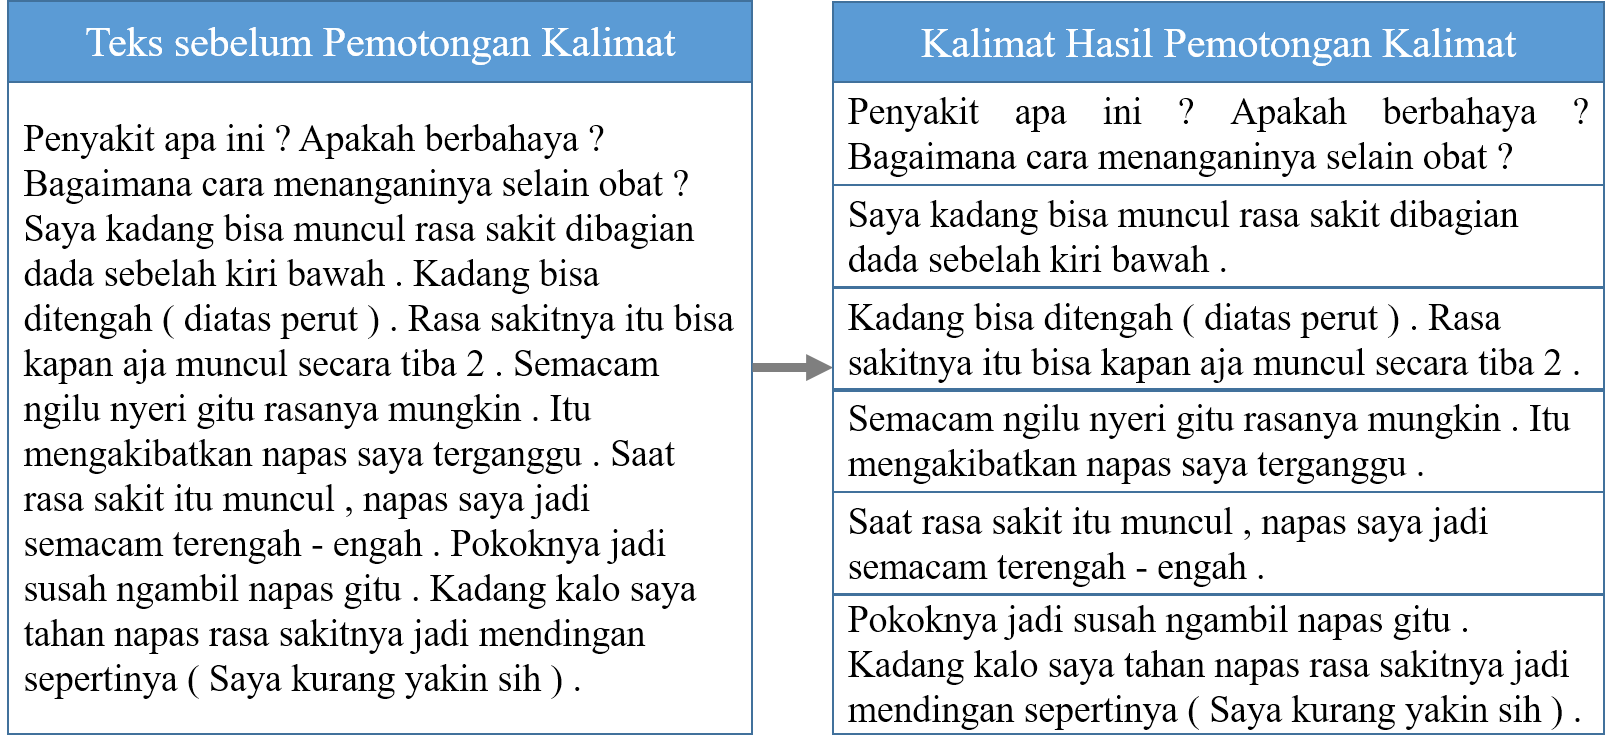
\includegraphics[width=\linewidth]{images/pemotongankalimat}
	\caption{Ilustrasi Pemotongan Kalimat pada suatu Teks}
	\label{fig:pemotongan_kalimat}
\end{figure}


\section{Pelabelan}
Pada tahap ini, \saya~melakukan pelabelan pada dokumen teks yang merupakan hasil pada tahap sebelumnya dengan label \disease, \symptom, \drug~dan \treatment. Berikut merupakan penjelasan dari masing-masing label:
\begin{enumerate}
	\item \Disease\\
	Entitas \disease~yang dimaksud pada penelitian ini yaitu nama dari suatu penyakit. Penyakit merupakan keadaan abnormal yang timbul pada tubuh manusia. Contoh dari entitas \disease~yaitu:
	\begin{description}
		\item[$\bullet$] Skizofrenia
		\item[$\bullet$] Trikotilomania
		\item[$\bullet$] Diabetes melitus
	\end{description}

	\item \Symptom\\
	Entitas \symptom~yang dimaksud pada penelitian ini yaitu fenomena yang dialami oleh seseorang yang terkena suatu penyakit. Contoh dari entitas \symptom~yaitu:
	\begin{description}
		\item[$\bullet$] Napas berbunyi
		\item[$\bullet$] Benjolan di daerah perut
		\item[$\bullet$] Nyeri saat BAK
	\end{description}

	\item \Drug\\
	Entitas \drug~merupakan entitas nama obat dari suatu penyakit yang memiliki fungsi untuk mengurangi atau menyembuhkan penyakit tersebut. Contoh dari entitas \drug~yaitu:
	\begin{description}
		\item[$\bullet$] Paracetamol
		\item[$\bullet$] Diltiazem
		\item[$\bullet$] eritropoetin-alfa
	\end{description}

	\item \Treatment\\
	Entitas \treatment~merupakan cara atau langkah penyembuhan dari suatu penyakit. Contoh dari entitas \treatment~yaitu:
	\begin{description}
		\item[$\bullet$] Pemeriksaan darah rutin
		\item[$\bullet$] Penilaian denyut kapiler
		\item[$\bullet$] Terapi inhalasi
	\end{description}

	\item \textit{Other}\\
	Entitas \textit{other} merupakan suatu entitas selain dari keempat entitas di atas. Contoh dari entitas \textit{other} yaitu:
	\begin{description}
		\item[$\bullet$] Saya
		\item[$\bullet$] yang
		\item[$\bullet$] Dokter
	\end{description}

\end{enumerate}
Setelah proses di atas selesai, label di dalam korpus diubah menjadi format BIO (\textit{begin inside outside}). Gambar \ref{fig:pelabelan} berikut merupakan ilustrasi dari tahap pelabelan ini.
\begin{figure}
	\centering
	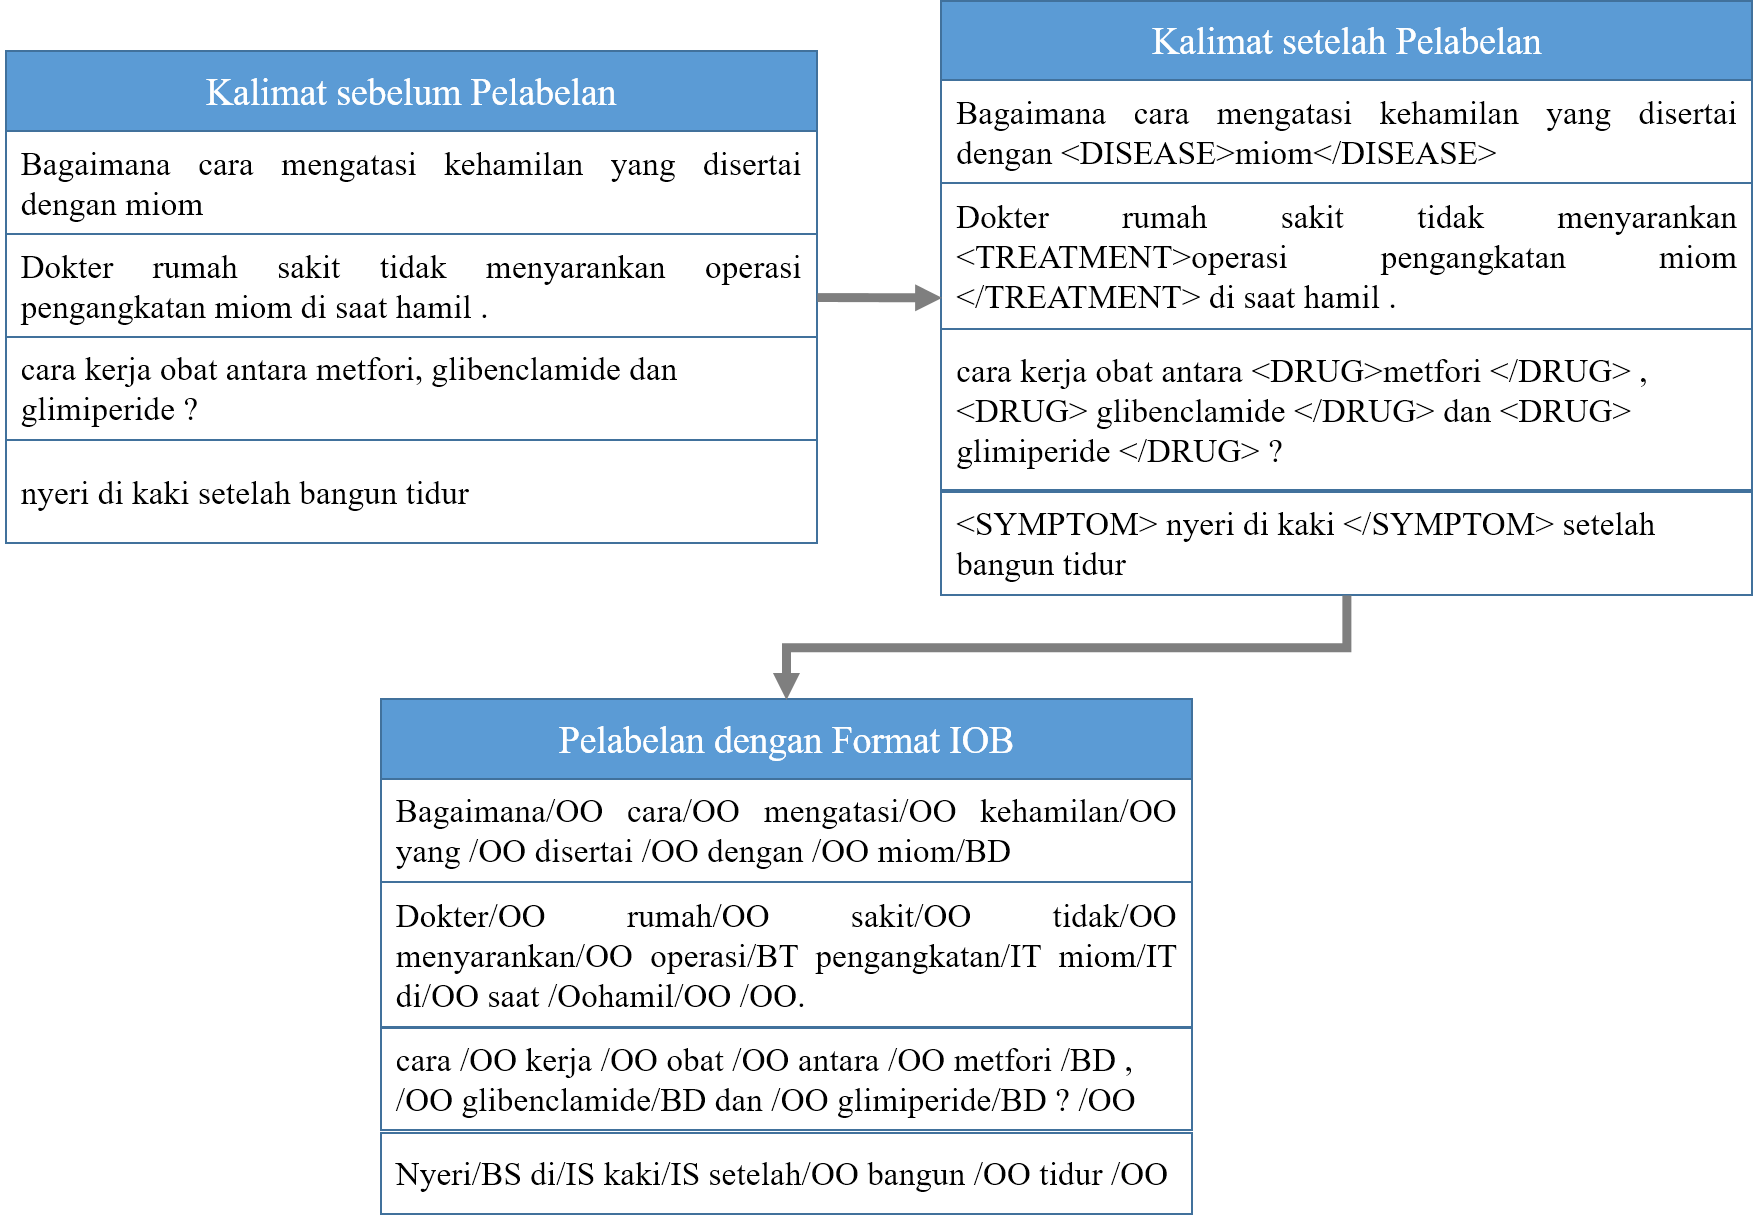
\includegraphics[width=\linewidth]{images/pelabelan}
	\caption{Ilustrasi Pelabelan Entitas pada suatu Kalimat}
	\label{fig:pelabelan}
\end{figure}

Setelah pelabelan selesai dilakukan, supaya model RNNs mampu mengenali masing-masing label, \saya~menggunakan \textit{one-hot-vector} untuk merepresentasikan masing-masing label. Tabel \ref{table:onehotlabel} merupakan tabel pemetaan dari label menjadi represebtasinya dalam \textit{one-hot-vector}.

\begin{table}
	\centering
	\caption{Tabel Pemetaan Label dengan Representasi \textit{One-Hot-Vector}}
	\label{table:onehotlabel}
	\begin{tabular}{|l|l|}
		\hline
		\multicolumn{1}{|c|}{Label IOB} & \multicolumn{1}{c|}{\textit{One-hot-vector}} \\ \hline
		BD & {[} 0, 0, 0, 0, 0, 0, 0, 0, 1 {]} \\ \hline
		ID & {[} 0, 0, 0, 0, 0, 0, 0, 1, 0 {]} \\ \hline
		BS & {[} 0, 0, 0, 0, 0, 0, 1, 0, 0 {]} \\ \hline
		IS & {[} 0, 0, 0, 0, 0, 1, 0, 0, 0 {]} \\ \hline
		BT & {[} 0, 0, 0, 0, 1, 0, 0, 0, 0 {]} \\ \hline
		IT & {[} 0, 0, 0, 1, 0, 0, 0, 0, 0 {]} \\ \hline
		BG & {[} 0, 0, 1, 0, 0, 0, 0, 0, 0 {]} \\ \hline
		IG & {[} 0, 1, 0, 0, 0, 0, 0, 0, 0 {]} \\ \hline
		OO & {[} 1, 0, 0, 0, 0, 0, 0, 0, 0 {]} \\ \hline
	\end{tabular}
\end{table}

Gambar \ref{fig:labeltoone} merupakan contoh pengubahan kata menjadi \textit{one-hot-vector} dalam suatu kalimat.

\begin{figure}
	\centering
	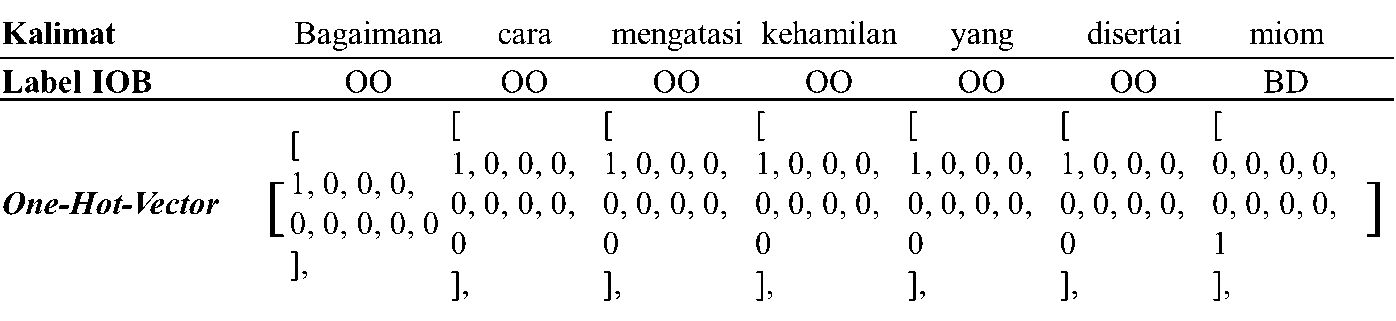
\includegraphics[width=\linewidth]{images/labeltoone}
	\caption{Ilustrasi Pengubahan Label menjadi \textit{One-Hot-Vector}}
	\label{fig:labeltoone}
\end{figure}

\section{Pengembangan Model}
Pada tahap ini, \saya~melakukan pengusulan dan perancangan model yang nantinya akan \saya~evaluasi pada tahap eksperimen. Dalam mengembangkan model, terdapat dua pekerjaan yang \saya~lakukan, yaitu:

\subsection{Ekstrasi Fitur}\label{subbab:fitur}
Pada tahap ini, \saya~melakukan ekstraksi fitur dari dokumen yang telah diberi label entitas. Ada beberapa fitur yang \saya~usulkan dalam penelitian ini yang nantinya \saya~kombinasikan supaya mendapatkan hasil terbaik. Fitur-fitur tersebut yaitu:
\begin{enumerate}
	\item Fitur 1: Kata itu sendiri\\
	Fitur ini merupakan fitur kata dalam representasi vektor. Fitur ini merupakan fitur yang digunakan \cite{abacha2011medical} dan \cite{skripsiKakRadit} dalam penelitian tentang \mer. Untuk mendapatkan representasi vektor dari masing-masing kata, penulis menggunakan \textit{word embedding}. Pada penelitian mengenai \mer~yang dilakukan oleh \cite{mujiono2016new}, hasil dari representasi data terbaik yaitu \textit{word embedding}. Selain itu, seperti yang dijelaskan pada Bab 2, \textit{word embedding} memberikan hasil yang sangat baik dalam bidang NLP. Oleh karena itu, \saya~menggunakan \textit{word embedding} untuk mendapatkan representasi vektor masing-masing kata. Dalam penelitian ini. Terdapat beberapa langkah yang perlu \saya~lakukan dalam memanfaatkan \textit{word embedding} ini, yaitu:
	\begin{enumerate}
		\item Pengumpulan data \textit{training} untuk \textit{word embedding}\\
		\Saya~melakukan pengumpulan data teks sebagai \textit{resource} untuk melakukan \textit{training} model \textit{word embedding}. Data teks yang \saya~gunakan merupakan data teks dari artikel-artikel kesehatan dan data teks forum kesehatan di kaskus. \Saya~menggunakan teks berjenis kesehatan supaya \textit{domain word embedding} dengan data \textit{training} untuk model \mer~sama. Selain itu, terdapat beberapa \textit{term} kesehatan yang susah ditemukan di forum umum.
		 
		\item \textit{Training} untuk mendapatkan model \textit{word embedding}\\
		\textit{Training} dilakukan untuk mendapatkan model yang mampu mendapatkan representasi vektor dari sebuah kata. Panjang vektor yang dihasilkan yaitu 128 dengan besaran \textit{window} yaitu 5. Arsitektur yang digunakan untuk melakukan \textit{training} ini adalah \textit{skip-gram}.
		
		\item Pengubahan kata menjadi vektor dari model yang didapatkan\\
		Pada langkah ini \saya~mengubah masing-masing kata dalam kalimat menjadi representasi vektor dengan model yang telah \saya~dapatkan pada tahap \textit{training} model \textit{word embedding}.
	\end{enumerate}
	
	Gambar \ref{fig:fiturkata} merupakan ilustrasi dari proses ekstraksi fitur kata itu sendiri dalam suatu kalimat dengan menggunakan \textit{Word Embedding}.
	
	\begin{figure}
		\centering
		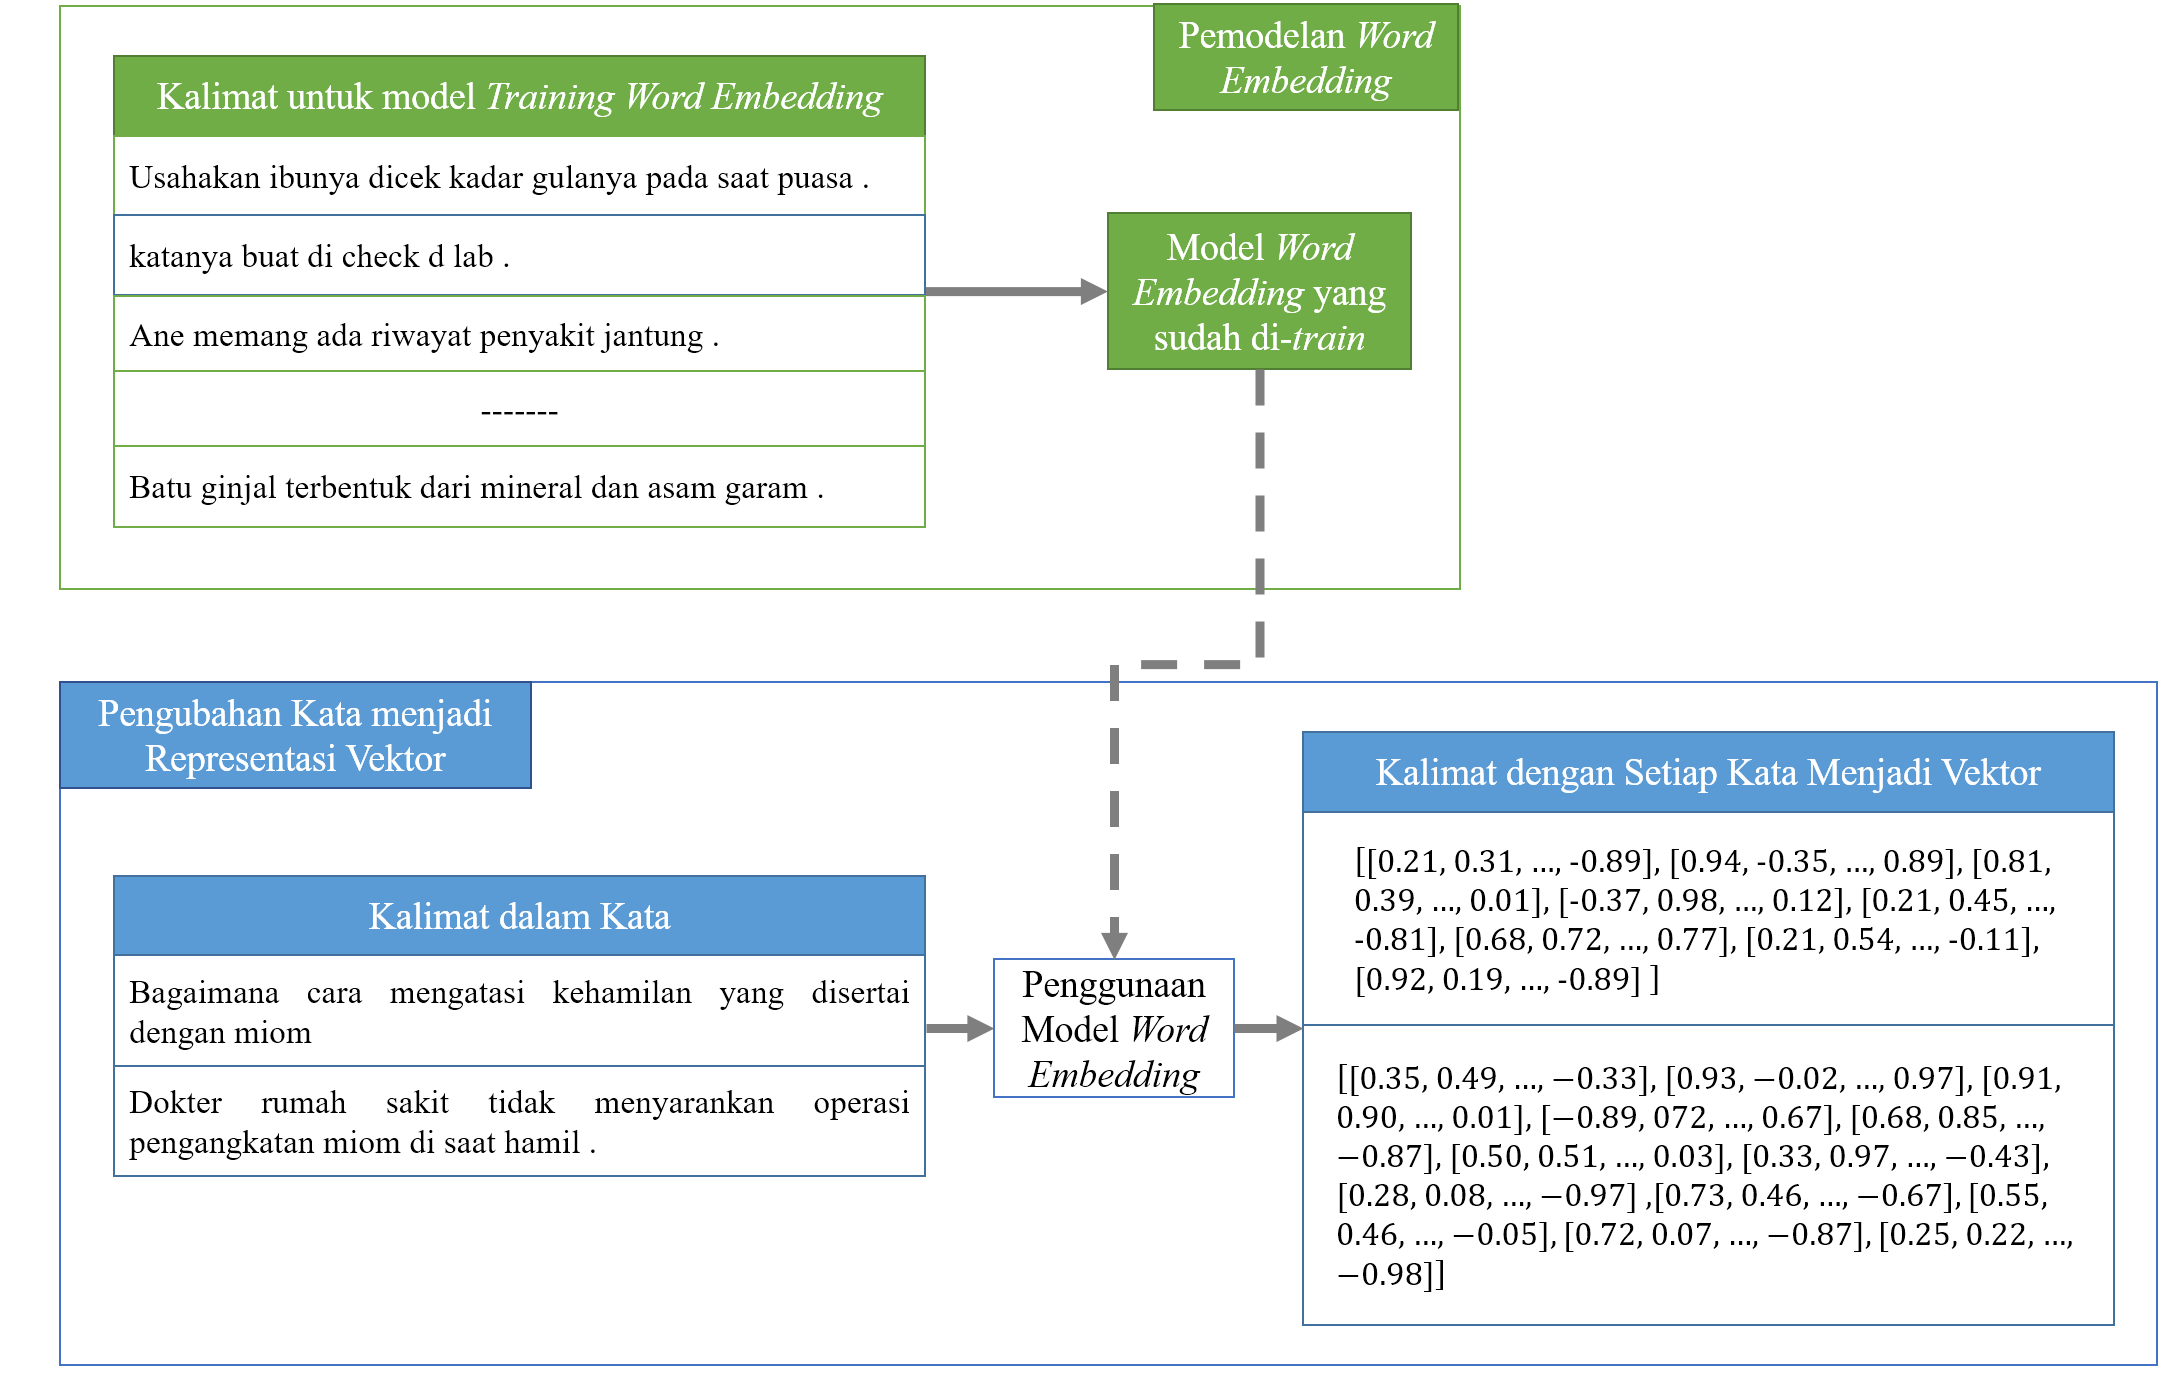
\includegraphics[width=\linewidth]{images/fiturkata}
		\caption{Ilustrasi Ekstraksi Fitur Kata pada Suatu Kalimat}
		\label{fig:fiturkata}
	\end{figure}
	
	\item Fitur 2: Kamus Kesehatan\\
	Fitur kamus kesehatan merupakan fitur yang berisi informasi suatu kata terdapat di dalam kamus kesehatan atau tidak. Fitur ini digunakan dalam penelitian \cite{skripsiKakRadit} dan memberikan kontribusi dalam hasil terbaik. Pada penelitian ini, kamus kesehatan yang dipakai merupakan kamus \disease, kamus \symptom, kamus \drug~dan kamus \treatment. Dengan menggunakan fitur ini diharapkan mampu berkontribusi dalam meningkatkan akurasi karena model akan mempertimbangkan apakah suatu kata termasuk di dalam kamus atau tidak. Gambar \ref{fig:fiturkamus} merupakan ilustrasi dari ekstraksi fitur kamus kesehatan dalam suatu kalimat.
	
	\begin{figure}
		\centering
		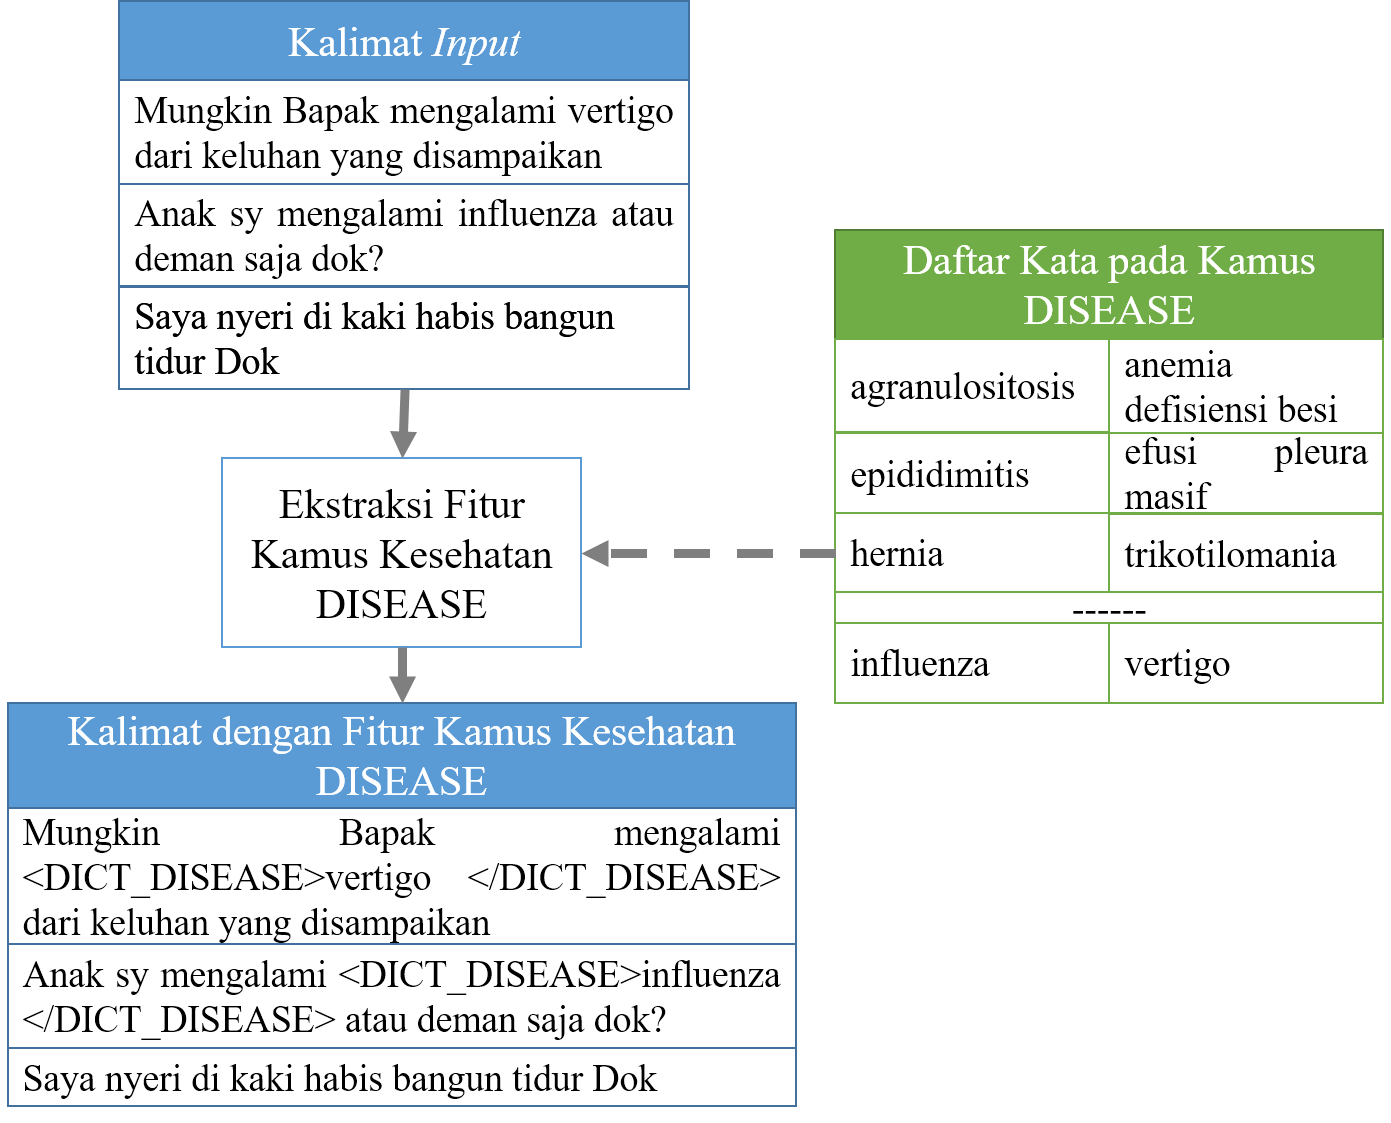
\includegraphics[width=\linewidth]{images/fiturkamus}
		\caption{Ilustrasi Ekstraksi Fitur Kamus \disease~pada Suatu Kalimat}
		\label{fig:fiturkamus}
	\end{figure}

	Supaya model RNNs mengenali fitur ini, \saya~menggunakan representasi \textit{one-hot vector}. Untuk suatu kata yang terdapat dalam kamus kesehatan, representasi vektornya adalah $ [0, 1] $, sedangkan yang tidak terdapat di dalam kamus kesehatan, representasi vektornya adalah $ [1, 0] $. Gambar \ref{fig:kamustoone} merupakan contoh pengubahan fitur kamus kesehatan menjadi representasi \textit{one-hot-vector}.
	
	\begin{figure}
		\centering
		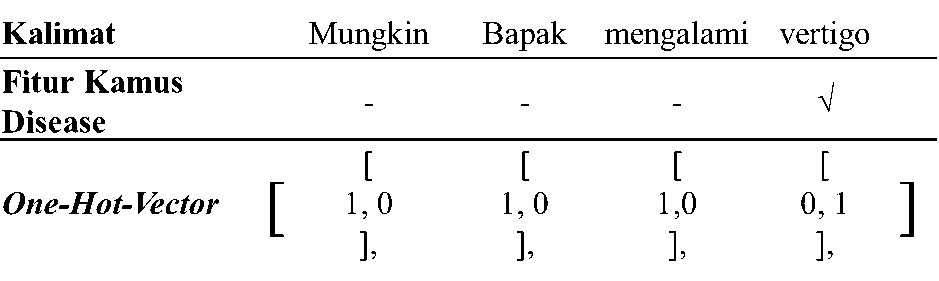
\includegraphics[width=0.85\linewidth]{images/kamustoone}
		\caption{Ilustrasi Pengubahan Label menjadi \textit{One-Hot-Vector}}
		\label{fig:kamustoone}
	\end{figure}
	
	\item Fitur 3: \textit{Stopword}\\
	Fitur ini merupakan fitur yang berisi vektor suatu kata merupakan \textit{stopword} atau bukan. Fitur ini \saya~gunakan dalam penelitian ini untuk membantu sistem dalam menghindari kesalahan pelabelan suatu kata yang bukan entitas namun dilabeli sebagai entitas.
	
	Ketika melakukan eksperimen, hasil yang \saya~dapatkan ternyata lebih bagus apabila mempertahankan fitur ini, oleh karena itu, \saya~mengusulkan untuk menggunakan fitur ini. Untuk pembahasan lebih lanjut dibahas pada Bab 5. Gambar \ref{fig:fiturstopword} merupakan ilustrasi dari ekstraksi fitur \textit{stopword} dalam suatu kalimat.
	
	\begin{figure}
		\centering
		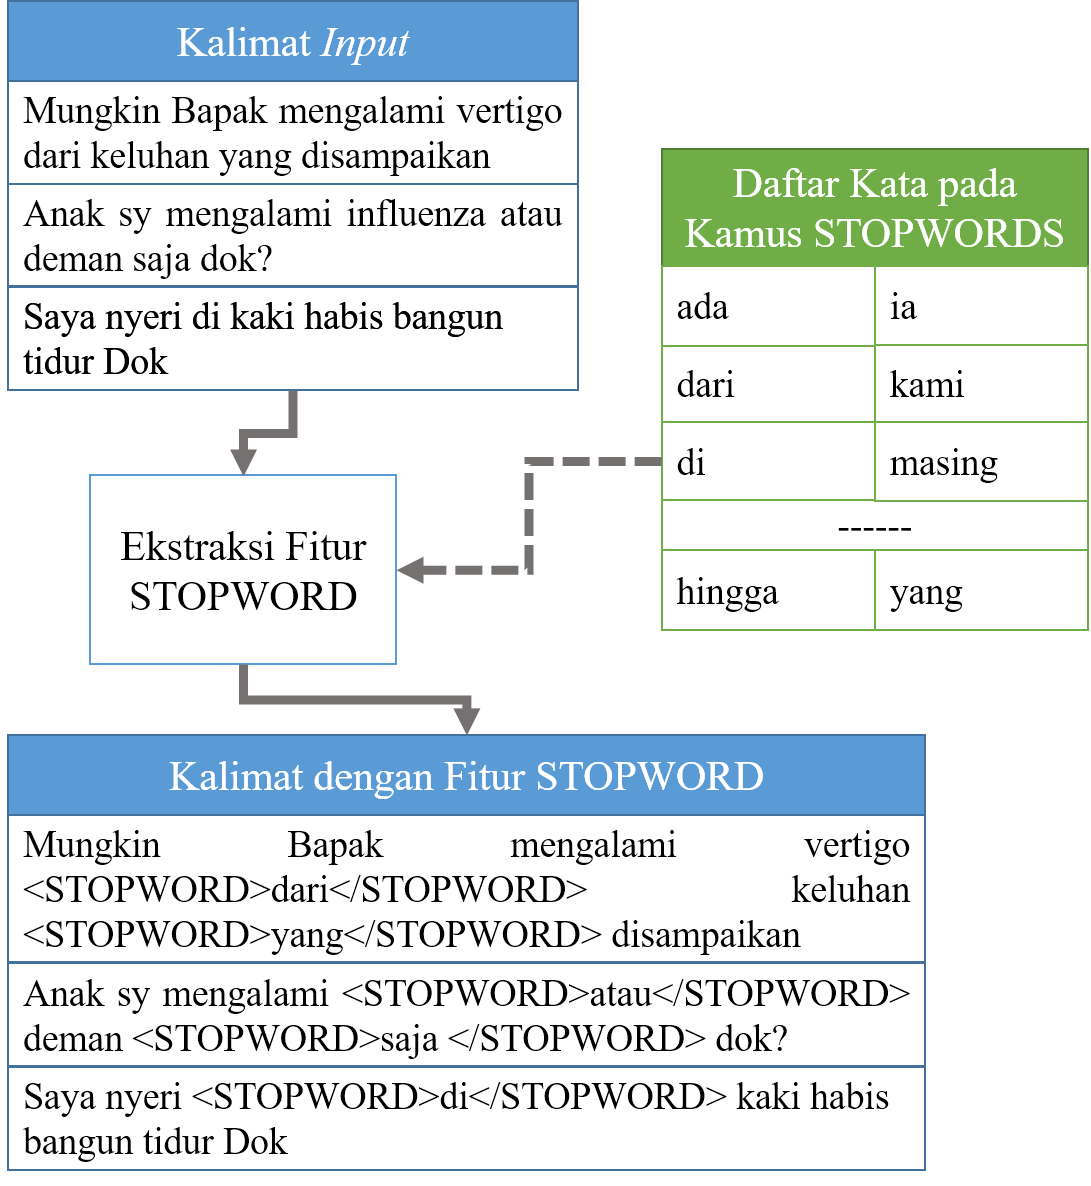
\includegraphics[width=\linewidth]{images/fiturstopword}
		\caption{Ilustrasi Ekstraksi Fitur \textit{Stopword} pada Suatu Kalimat}
		\label{fig:fiturstopword}
	\end{figure}

	Supaya model RNNs mengenali fitur ini, \saya~menggunakan representasi \textit{one-hot vector}. Untuk suatu kata yang merupakan \textit{stopword}, representasi vektornya adalah $ [0, 1] $, sedangkan yang bukan merupakan \textit{stopword}, representasi vektornya adalah $ [1, 0] $. Gambar \ref{fig:stopwordtoone} merupakan contoh pengubahan fitur \textit{stopword} menjadi representasi \textit{one-hot-vector}.
	
	\begin{figure}
		\centering
		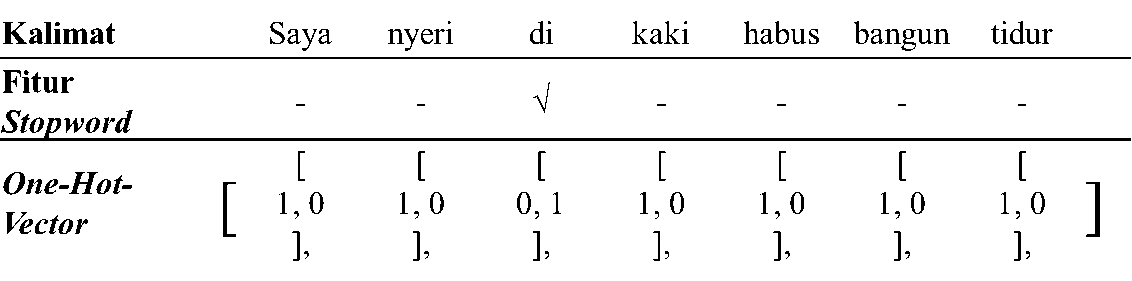
\includegraphics[width=0.85\linewidth]{images/stopwordtoone}
		\caption{Ilustrasi Pengubahan Label menjadi \textit{One-Hot-Vector}}
		\label{fig:stopwordtoone}
	\end{figure}

	\item Fitur 4: \textit{Part of Speech Tag} (POS-Tag)\\
	Fitur ini merupakan fitur \textit{tag} yang dimiliki setiap kata yang diusulkan oleh \cite{abacha2011medical} dalam penelitiannya di bidang \mer. Entitas-entitas tertentu memiliki tag yang sama, misalnya entitas obat dan penyakit pada umumnya memiliki tag "NNP" sehingga dengan digunakannya fitur ini sistem dapat mengenali jenis obat dan penyakit dengan lebih baik. Model POS-Tagger yang \saya~gunakan merupakan model POS-Tag berbahasa Indonesia. Gambar \ref{fig:fiturpostag} merupakan ilustrasi dari ekstraksi fitur POS-\textit{Tag} dalam suatu kalimat.
	
	\begin{figure}
		\centering
		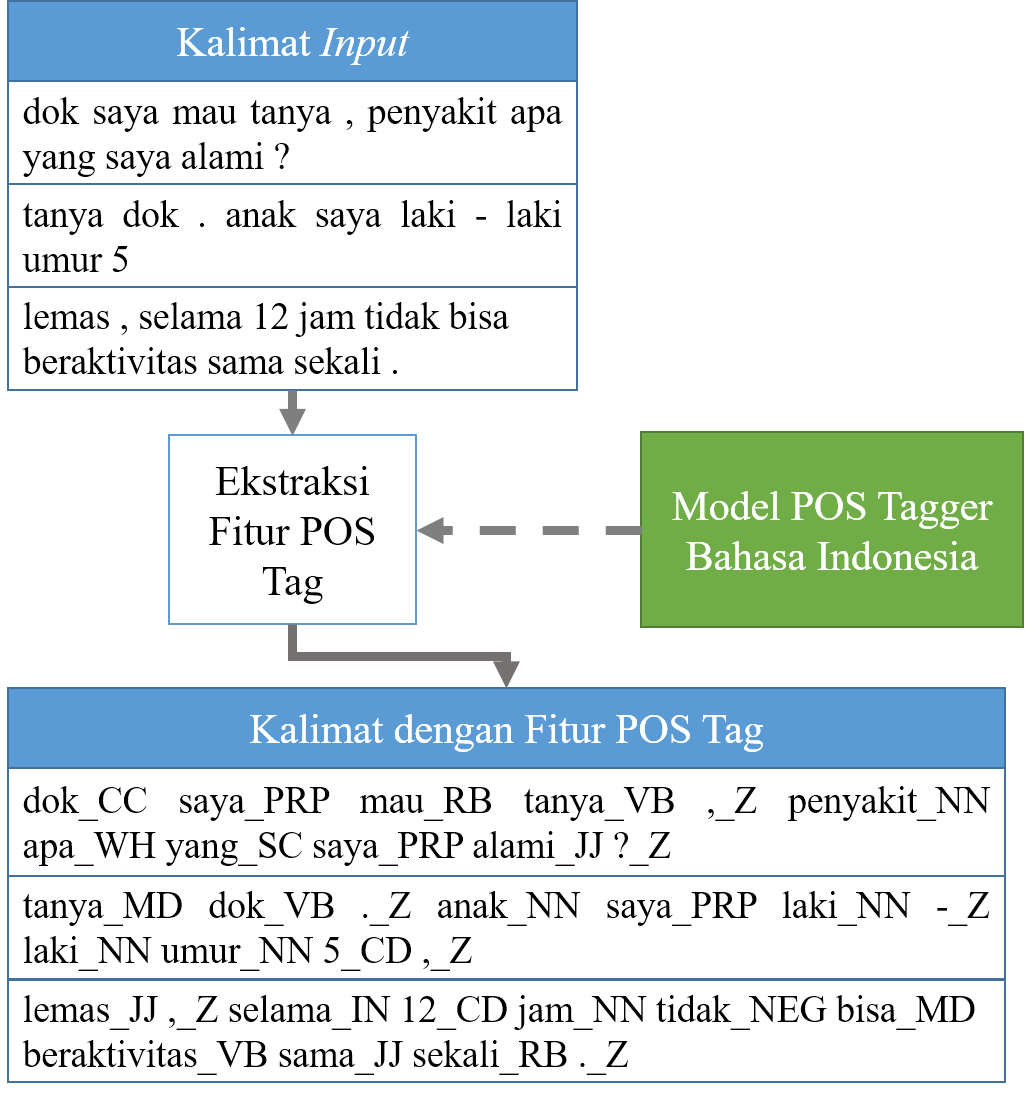
\includegraphics[width=\linewidth]{images/fiturpostag}
		\caption{Ilustrasi Ekstraksi Fitur POS \textit{Tag} pada Suatu Kalimat}
		\label{fig:fiturpostag}
	\end{figure}

	Setelah POS-Tag didapatkan, supaya model RNNs mampu mengenali masing-masing tag, \saya~menggunakan \textit{one-hot-vector} untuk merepresentasikan masing-masing label. Tabel \ref{table:onehotpostag} merupakan tabel pemetaan dari label menjadi representasinya dalam \textit{one-hot-vector}.
	
	\begin{table}
		\centering
		\caption{Tabel Pemetaan POS-Tag dengan Representasi \textit{One-Hot-Vector}}
		\label{table:onehotpostag}
		\begin{tabular}{|l|l|}
			\hline
			\multicolumn{1}{|c|}{Label POS-Tag} & \multicolumn{1}{c|}{\textit{One-hot-vector}} \\ \hline
			JJ & {[}0,0,0,0,0,0,0,0,0,0,0,0,0,0,0,0,0,0,0,0,0,0,0,1{]} \\ \hline
			NN & {[}0,0,0,0,0,0,0,0,0,0,0,0,0,0,0,0,0,0,0,0,0,0,1,0{]} \\ \hline
			NNP & {[}0,0,0,0,0,0,0,0,0,0,0,0,0,0,0,0,0,0,0,0,0,1,0,0{]} \\ \hline
			Z & {[}0,0,0,0,0,0,0,0,0,0,0,0,0,0,0,0,0,0,0,0,1,0,0,0{]} \\ \hline
			IN & {[}0,0,0,0,0,0,0,0,0,0,0,0,0,0,0,0,0,0,0,1,0,0,0,0{]} \\ \hline
			PRP & {[}0,0,0,0,0,0,0,0,0,0,0,0,0,0,0,0,0,0,1,0,0,0,0,0{]} \\ \hline
			MD & {[}0,0,0,0,0,0,0,0,0,0,0,0,0,0,0,0,0,1,0,0,0,0,0,0{]} \\ \hline
			VB & {[}0,0,0,0,0,0,0,0,0,0,0,0,0,0,0,0,1,0,0,0,0,0,0,0{]} \\ \hline
			SC & {[}0,0,0,0,0,0,0,0,0,0,0,0,0,0,0,1,0,0,0,0,0,0,0,0{]} \\ \hline
			RB & {[}0,0,0,0,0,0,0,0,0,0,0,0,0,0,1,0,0,0,0,0,0,0,0,0{]} \\ \hline
			CC & {[}0,0,0,0,0,0,0,0,0,0,0,0,0,1,0,0,0,0,0,0,0,0,0,0{]} \\ \hline
			NEG & {[}0,0,0,0,0,0,0,0,0,0,0,0,1,0,0,0,0,0,0,0,0,0,0,0{]} \\ \hline
			WH & {[}0,0,0,0,0,0,0,0,0,0,0,1,0,0,0,0,0,0,0,0,0,0,0,0{]} \\ \hline
			CD & {[}0,0,0,0,0,0,0,0,0,0,1,0,0,0,0,0,0,0,0,0,0,0,0,0{]} \\ \hline
			X & {[}0,0,0,0,0,0,0,0,0,1,0,0,0,0,0,0,0,0,0,0,0,0,0,0{]} \\ \hline
			PR & {[}0,0,0,0,0,0,0,0,1,0,0,0,0,0,0,0,0,0,0,0,0,0,0,0{]} \\ \hline
			RP & {[}0,0,0,0,0,0,0,1,0,0,0,0,0,0,0,0,0,0,0,0,0,0,0,0{]} \\ \hline
			FW & {[}0,0,0,0,0,0,1,0,0,0,0,0,0,0,0,0,0,0,0,0,0,0,0,0{]} \\ \hline
			NND & {[}0,0,0,0,0,1,0,0,0,0,0,0,0,0,0,0,0,0,0,0,0,0,0,0{]} \\ \hline
			DT & {[}0,0,0,0,1,0,0,0,0,0,0,0,0,0,0,0,0,0,0,0,0,0,0,0{]} \\ \hline
			OD & {[}0,0,0,1,0,0,0,0,0,0,0,0,0,0,0,0,0,0,0,0,0,0,0,0{]} \\ \hline
			UH & {[}0,0,1,0,0,0,0,0,0,0,0,0,0,0,0,0,0,0,0,0,0,0,0,0{]} \\ \hline
			SYM & {[}0,1,0,0,0,0,0,0,0,0,0,0,0,0,0,0,0,0,0,0,0,0,0,0{]} \\ \hline
			fw & {[}1,0,0,0,0,0,0,0,0,0,0,0,0,0,0,0,0,0,0,0,0,0,0,0{]} \\ \hline
		\end{tabular}
	\end{table}

	Gambar \ref{fig:postagtoone} merupakan contoh pengubahan fitur POS-Tag menjadi \textit{one-hot-vector} dalam suatu kalimat.
	
	\begin{figure}
		\centering
		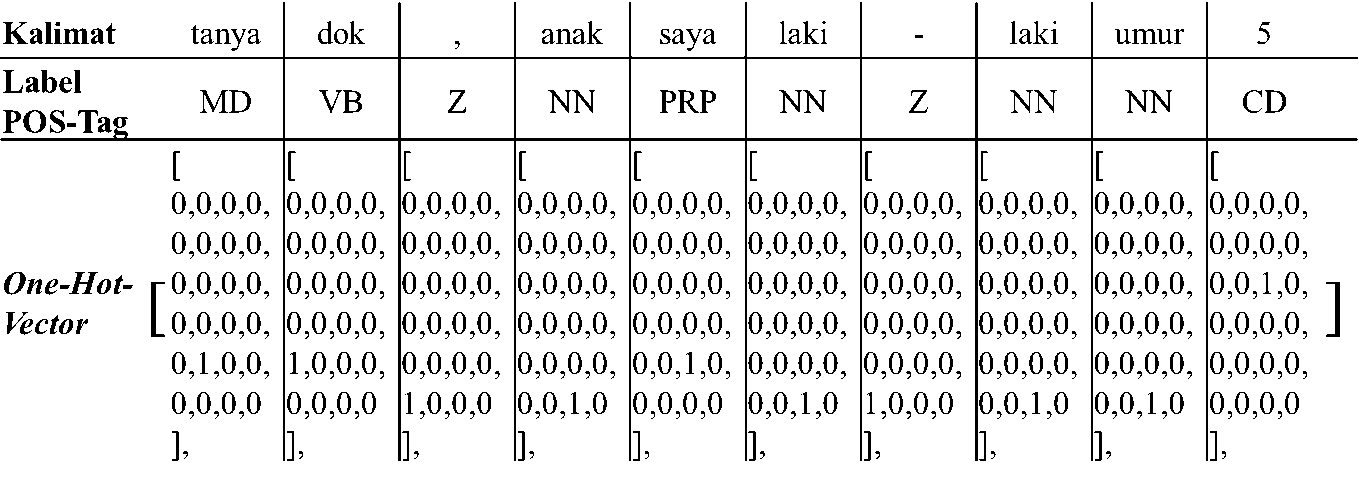
\includegraphics[width=\linewidth]{images/postagtoone}
		\caption{Ilustrasi Pengubahan Fitur POS-Tag menjadi \textit{One-Hot-Vector}}
		\label{fig:postagtoone}
	\end{figure}
		
	\item Fitur 5: Frasa Kata\\
	Pada penelitian ini, \saya~mengusulkan fitur frasa kata karena entitas \textit{symptom} dan \textit{treatment}  pada umumnya merupakan frasa kata kerja. Sedangkan entitas \textit{disease} dan \textit{drug} pada umumnya entitas yang akan dikenali pada penelitian ini merupakan frasa kata benda. Selain itu, pada penelitian \cite{skripsiKakRadit}, fitur ini berkontribusi dalam memberikan hasil terbaik. Oleh karena itu, \saya~berharap bahwa dengan diusulkannya fitur ini akan mampu menambah akurasi dari model yang diusulkan.
	
	Pada penelitian ini ada dua frasa yang diujicobakan, yaitu:
	\begin{enumerate}
		\item Frasa Kata Benda (Nomina)
		Menurut \cite{hs2005bahasa}, frasa kata benda sendiri merupakan kelompok kata benda yang dibentuk dengan memperluas kata benda ke sekelilingnya. Fitur frasa kata benda yang \saya~gunakan dalam penelitian merupakan fitur yang berisi informasi suatu kata atau kumpulan kata merupakan frasa kata benda atau bukan. Dalam menentukan suatu kata merupakan frasa atau bukan, penulis menggunakan aturan pembentukan frasa yang digunakan pada bahasa Indonesia, yaitu:
		\begin{description}
			\item[$\bullet$] NP : NN
			\item[$\bullet$] NP : NNP
			\item[$\bullet$] NP : PR
			\item[$\bullet$] NP : PRP
			\item[$\bullet$] NP : NN + NN
			\item[$\bullet$] NP : NN + NNP
			\item[$\bullet$] NP : NN + PR
			\item[$\bullet$] NP : NN + PRP
			\item[$\bullet$] NP : NN + JJ
			\item[$\bullet$] NP : DT + NN
			\item[$\bullet$] NP : RB + NN
			\item[$\bullet$] NP : CD + NN
			\item[$\bullet$] NP : NND + NN
		\end{description}
		
		\item Frasa Kata Kerja (Verbal)\\
		Menurut \cite{hs2005bahasa}, frasa verbal merupakan kelompok kata benda yang dibentuk dengan kata kerja. Fitur frasa verbal yang \saya~gunakan dalam penelitian merupakan fitur yang berisi informasi suatu kata atau kumpulan kata merupakan frasa verbal atau bukan. Dalam menentukan suatu kata merupakan frasa atau bukan, penulis menggunakan aturan pembentukan frasa yang digunakan pada bahasa Indonesia, yaitu:
		\begin{description}
			\item[$\bullet$] VP : VB
			\item[$\bullet$] VP : VB + NP
		\end{description}
	\end{enumerate}

Gambar \ref{fig:fiturfrasa} merupakan ilustrasi dari ekstraksi fitur Frasa Nomina dalam suatu kalimat.

\begin{figure}
	\centering
	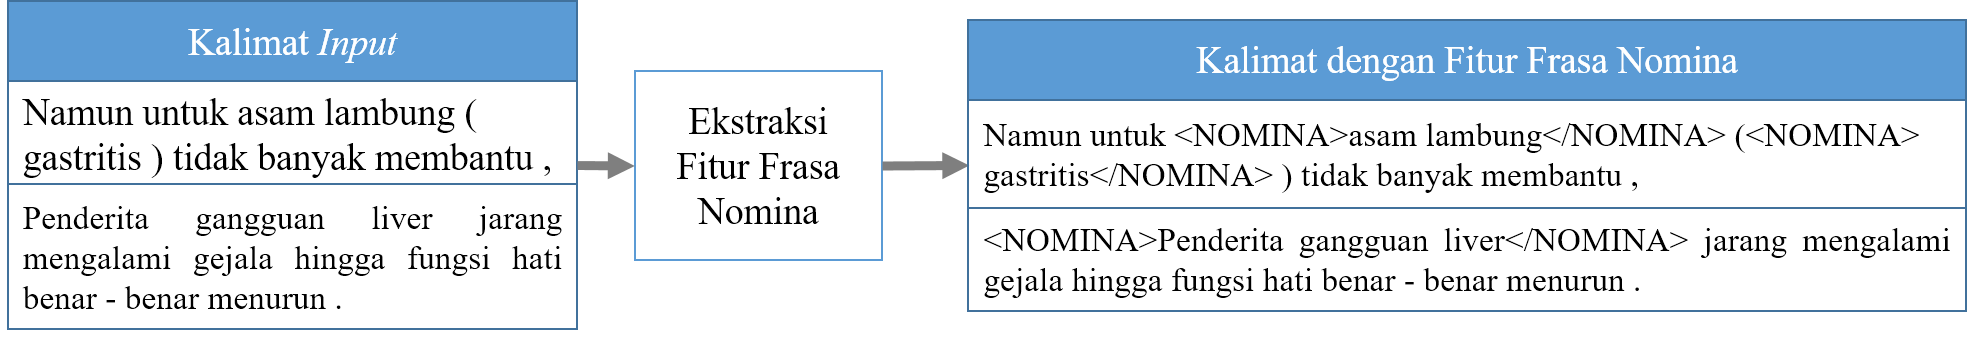
\includegraphics[width=\linewidth]{images/fiturfrasa}
	\caption{Ilustrasi Ekstraksi Fitur Frasa Nomina pada Suatu Kalimat}
	\label{fig:fiturfrasa}
\end{figure}

Supaya model RNNs mengenali fitur ini, \saya~menggunakan representasi \textit{one-hot vector}. Untuk suatu kata yang merupakan sebuah frasa, representasi vektornya adalah $ [0, 1] $, sedangkan yang bukan, representasi vektornya adalah $ [1, 0] $. Gambar \ref{fig:frasatoone} merupakan contoh pengubahan fitur frasa nomina menjadi representasi \textit{one-hot-vector}.

\begin{figure}
	\centering
	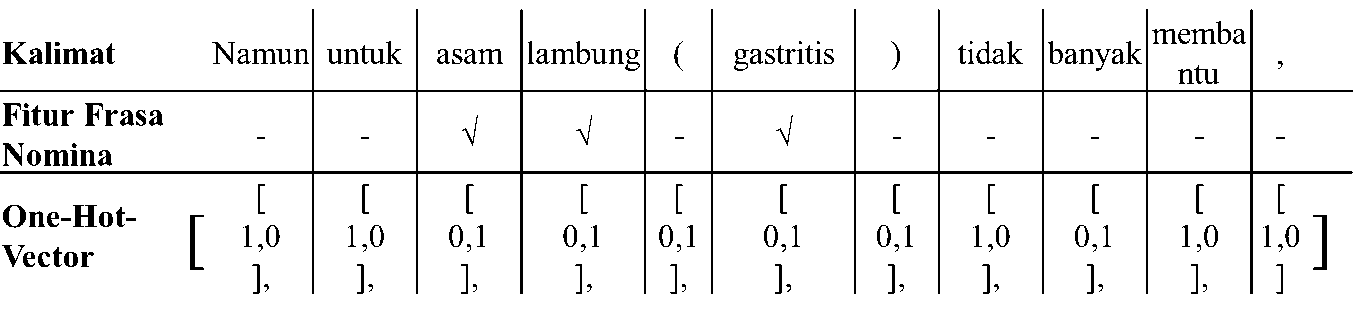
\includegraphics[width=0.85\linewidth]{images/frasatoone}
	\caption{Ilustrasi Pengubahan Fitur Frasa menjadi \textit{One-Hot-Vector}}
	\label{fig:frasatoone}
\end{figure}

 \item Fitur 6: 1 Kata Sebelum\\
 Fitur ini merupakan fitur yang berisi informasi kata sebelum kata saat ini yang direpresentasikan dalam bentuk vektor untuk masing-masing kata. Fitur ini digunakan pada penelitian penelitian \cite{skripsiKakRadit} yang juga berkontribusi memberikan hasil terbaik pada penelitiannya. Menurut \saya, ada beberapa entitas yang akan lebih mudah diketahui apabila diketahui kata sebelumnya. Misalnya kata "masuk angin", apabila hanya diberikan informasi kata "angin" tanpa kata "masuk", akan lebih sulit menentukan kata tersebut bagian dari suatu entitas \textit{disease} atau bukan.
  
 \item Fitur 7: 1 Kata Sesudah\\
 Fitur ini merupakan fitur yang berisi informasi kata sesudah kata saat ini yang direpresentasikan dalam bentuk vektor untuk masing-masing kata. Sama seperti pada fitur 1 Kata Sebelum, ada beberapa kasus yang mana apabila suatu kata merupakan sebuah entitas, akan lebih mudah dikenali apabila melihat kata atau konteks setelahnya. Sama seperti contoh pada Fitur 1 Kata Sebelum, misal diberikan kata "masuk angin", apabila hanya diberikan informasi "masuk" tanpa "angin", akan lebih sulit mengenali apakah kata tersebut termasuk entitas \textit{disease} atau bukan. Selain itu, fitur ini juga dapat membedakan kata berentitas dengan kata yang bukan, misalnya kata "masuk angin" dengan "masuk rumah". Apabila informasi pada saat tersebut hanya diberikan kata "masuk" saja tanpa kata setelahnya, akan lebih sulit mengenali kata tersebut termasuk kata berentitas atau bukan.
  
\end{enumerate}

\subsection{Pengusulan Arsitektur RNNs}
Pada tahap ini \saya~mengusulkan arsitektur RNNs yang akan digunakan pada tahap eksperimen. Ada dua arsitektur yang \saya~gunakan dalam penelitian ini, yaitu
\begin{enumerate}
	\item LSTMs 1 layer\\
	Pada LSTMs 1 layer, semua fitur yang menjadi input pada sebuah \textit{timestep} digabung menjadi satu. Untuk menentukan label, \saya~menggunakan \textit{feed-forward Neural Networks} pada masing-masing \textit{timestep} di layer terakhir. Berikut merupakan ilustrasi LSTM 1 layer yang \saya~gunakan dalam penelitian ini.
	
	\begin{figure}
		\centering
		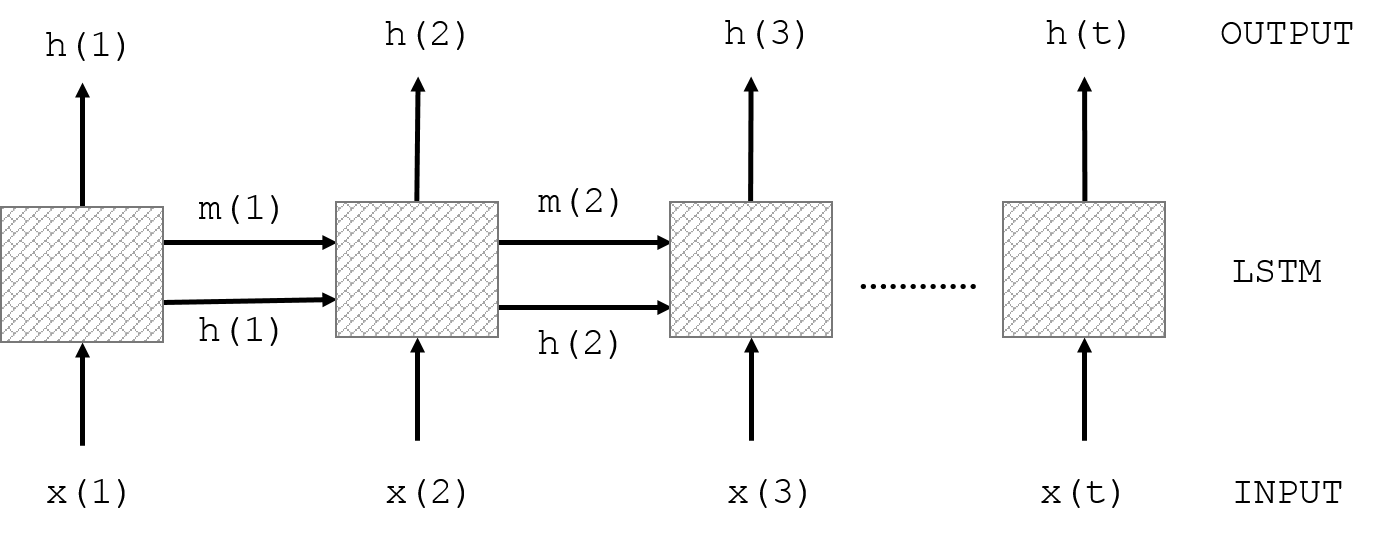
\includegraphics[width=0.8\linewidth]{images/lstm1}
		\caption{LSTMs 1 layer}
		\label{fig:single_layer_rnn}
	\end{figure}

	Misalnya fitur yang digunakan adalah fitur kata dan frasa. Karena hanya terdapat 1 layer saja, kedua fitur ini digabung terlebih dahulu menjadi 1. Gambar \ref{fig:inputlstm} merupakan ilustrasi dari proses penggabungan fitur supaya menjadi \textit{input} RNNs, dan  \textit{output} serta pemetaan menjadi label pada arsitektur ini.
	\begin{figure}
		\centering
		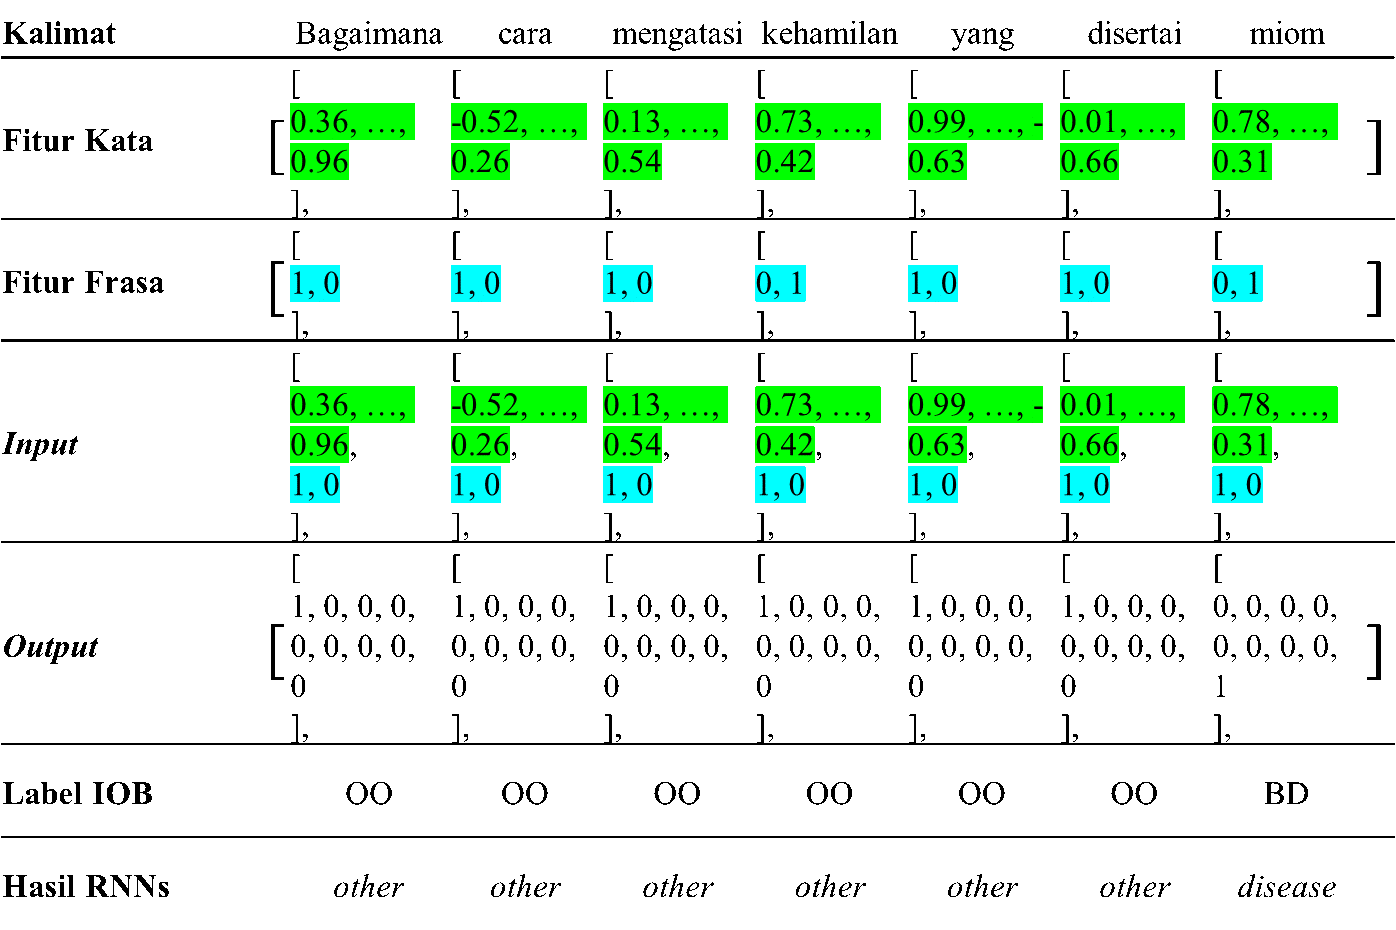
\includegraphics[width=0.85\linewidth]{images/concatlstm1}
		\caption{Ilustrasi penggabungan fitur kata dan frasa untuk menjadi \textit{input} LSTMs 1 layer dan \textit{output}-nya}
		\label{fig:inputlstm}
	\end{figure}
	
	Untuk masing-masing \textit{timestep} $ t $, berikut merupakan gambar sebuah \textit{cell}-nya.
	\begin{figure}
		\centering
		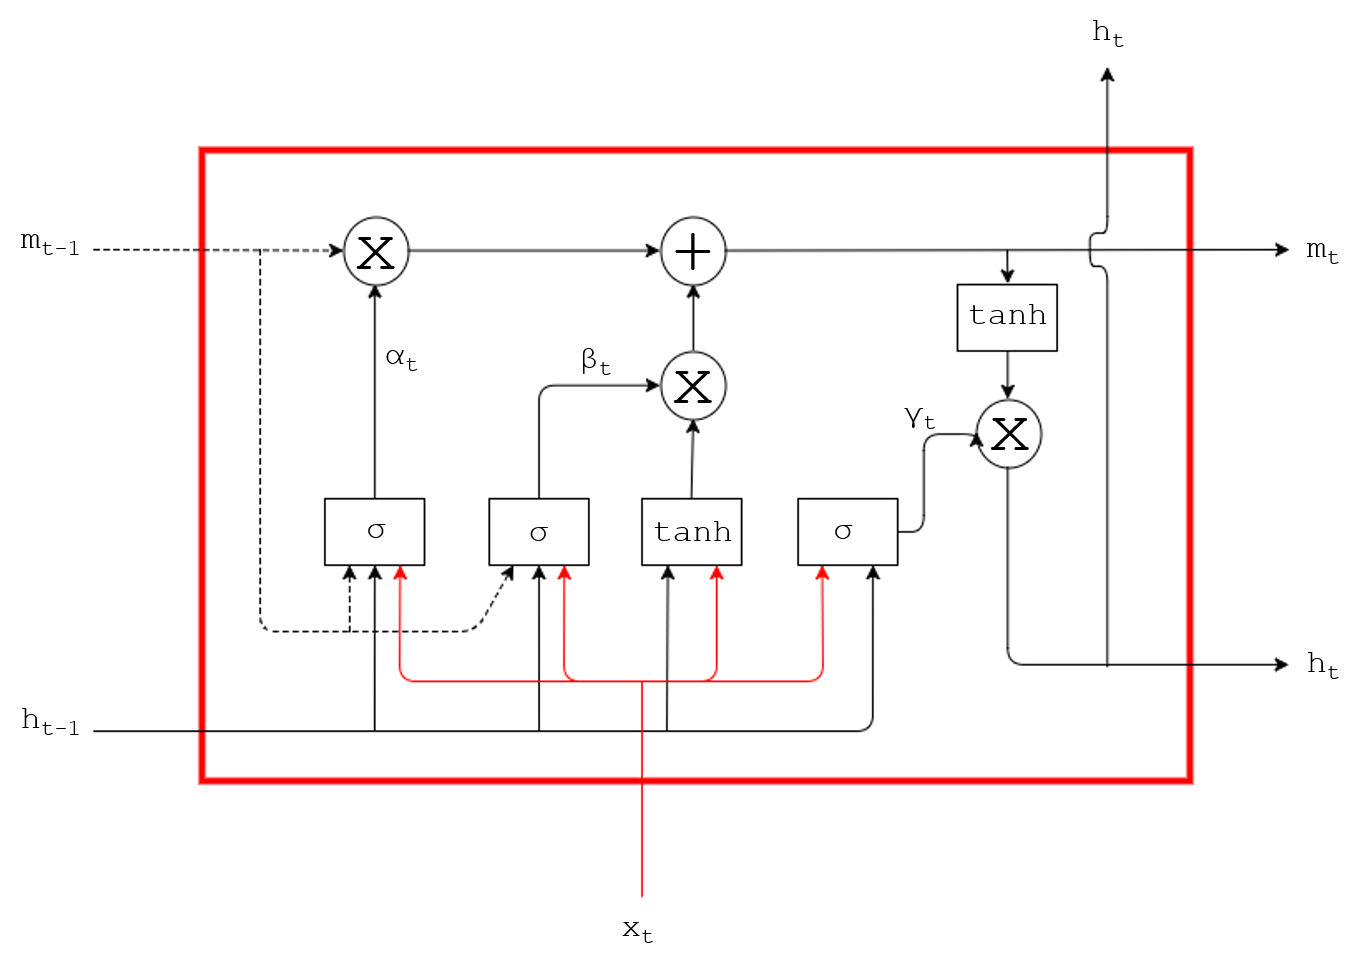
\includegraphics[width=0.85\linewidth]{images/lstm}
		\caption{1 buah blok memori dalam LSTM}
		\label{fig:lstm1cell}
	\end{figure}
	
	Dari gambar \ref{fig:lstm1cell}, sebuah \textit{cell} membutuhkan \textit{input} $ x(t) $ dan \textit{output} $ h(t) $. $ x(t) $ merupakan vektor dengan panjang $ N $, dan $ h(t) $ merupakan vektor dengan panjang $ M $. Seperti yang telah dijelaskan pada subbab \ref{subbab:lstm}, berikut merupakan formula untuk mengetahui \textit{output} pada \textit{timestep} $ t $.
	\begin{equation}\label{eq:lstmm}
	m_{t}=\alpha_{t} (\times) m_{t-1} + \beta_{t} (\times) f(x_{t},{t-1})
	\end{equation}
	\begin{equation}\label{eq:lstmh}
	h_{t}=\gamma_{t} (\times) tanh(m_{t})
	\end{equation}
	dimana
	\begin{equation}\label{eq:lstmx}
	f(x_{t},{t-1})=tanh(W_{xm} \cdot x_{t} + W_{hm} \cdot h_{t-1})
	\end{equation}
	
	$ \alpha_t $, $ \beta_t $ dan $ \gamma_t $ merupakan \textit{gates}:
	\begin{enumerate}
		\item \textit{Forget gates}: $ \alpha_{t}=\sigma(W_{x\alpha}+W_{h\alpha}\cdot~h_{t-1}+W_{m\alpha}\cdot~m_{t-1}) $
		\item \textit{Input gates}: $ \beta_{t}=\sigma(W_{x\beta}+W_{h\beta}\cdot~h_{t-1}+W_{m\beta}\cdot~m_{t-1}) $
		\item \textit{Output gates}: $ \gamma_{t}=\sigma(W_{x\gamma}+W_{h\gamma}\cdot~h_{t-1}+W_{m\gamma}\cdot~m_{t-1}) $
	\end{enumerate}

	\item LSTMs 2 layer dengan Multi-\textit{Input}\\
	Pada LSTMs 2 layer dengan multi-\textit{input}, penulis mendefinisikan 2 layer, yang layer terbawah merupakan layer dengan jumlah LSTMs sebanyak n kelompok fitur. Pertama-tama fitur dikelompokkan terlebih dahulu, kemudian dijadikan \textit{input} untuk masing-masing LSTMs pada tingkat pertama. Setelah itu, hasil dari tingkat pertama tersebut akan digabung menjadi satu, dengan menggunakan layer penggabung (\textit{Merge Layer}). \textit{Output} dari layer penggabung kemudian dimasukkan ke dalam LSTMs layer kedua. Untuk menentukan label, \saya~menggunakan \textit{feed-forward Neural Network} pada masing-masing \textit{timestep} di layer terakhir. Berikut merupakan ilustrasi dari LSTMs layer bertingkat yang \saya~gunakan.
	
	\begin{figure}
		\centering
		\includegraphics[width=1.0\linewidth]{images/lstm2}
		\caption{LSTM 2 layer}
		\label{fig:lstm2}
	\end{figure}

	Masing-masing kelompok fitur menjadi \textit{input} dari LSTMs yang terkait. Nantinya, masing-masing \textit{output} akan digabung melalui \textit{merge layer} dengan metode \textit{concat} dan menjadi \textit{input} bagi LSTMs layer kedua.
	Di sini, \saya~menotasikan $ k $ sebagai nomor kelompok fitur dan $ t $ sebagai \textit{timestep} saat ini. Untuk masing-masing kelompok fitur, berikut merupakan formulasi \textit{feedforward}-nya:
	\begin{equation}\label{eq:mt2}
	m_{k,t}=\alpha_{k,t} (\times) m_{k,t-1} + \beta_{k,t} (\times) f(x_{k,t},{k,t-1})
	\end{equation}
	\begin{equation}\label{eq:ht2}
	h_{k,t}=\gamma_{k,t} (\times) tanh(k,m_{t})
	\end{equation}
	dimana
	\begin{equation}\label{eq:hf2}
	f(x_{k,t},{k,t-1})=tanh(W_{k,xm} \cdot x_{t} + W_{k,hm} \cdot h_{k,t-1})
	\end{equation}
	$ \alpha_{k,t} $, $ \beta_{k,t} $ dan $ \gamma_{k,t} $ merupakan \textit{gates}:
	\begin{enumerate}
	\item \textit{Forget gates}: $ \alpha_{k,t}=\sigma(W_{k,x\alpha}+W_{k,h\alpha}\cdot~h_{k,t-1}+W_{k,m\alpha}\cdot~m_{k,t-1}) $
	\item \textit{Input gates}: $ \beta_{k,t}=\sigma(W_{k,x\beta}+W_{k,h\beta}\cdot~h_{k,t-1}+W_{k,m\beta}\cdot~m_{k,t-1}) $
	\item \textit{Output gates}: $ \gamma_{k,t}=\sigma(W_{k,x\gamma}+W_{k,h\gamma}\cdot~h_{k,t-1}+W_{k,m\gamma}\cdot~m_{k,t-1}) $
	\end{enumerate}

	\textit{Merge layer} berfungsi untuk menggabungkan hasil dari \textit{feedforward} pada semua LSTMs layer pertama. Di sini, \saya~menotasikan $ X_t $ sebagai hasil dari \textit{merge} di \textit{timestep} $ t $ dan $ (\cdot) $ merupakan operasi \textit{merging}.
	\begin{equation}\label{eq:merge}
	X_t = h_{1,t} (\cdot) h_{2,t} (\cdot) h_{3,t} (\cdot) .... (\cdot) h_{k,t}
	\end{equation}

	Hasil dari \textit{merge layer} akan digunakan sebagai \textit{input} bagi LSTMs layer kedua. Untuk memudahkan penggunaan notasi dan membedakan dengan LSTMs pada layer pertama, \saya~menggunakan huruf kapital dalam menotasikan masing-masing nilai di LSTMs layer kedua. Berikut merupakan formulasi \textit{feed-forwarnya}.
	
	\begin{equation}\label{eq:mt3}
	M_{t}=\alpha_{t} (\times) M_{t-1} + \beta_{t} (\times) f(X_{t},{t-1})
	\end{equation}
	\begin{equation}\label{eq:ht3}
	H_{t}=\gamma_{t} (\times) tanh(M_{t})
	\end{equation}
	dimana
	\begin{equation}\label{eq:hf3}
	f(X_{t},{t-1})=tanh(W_{XM} \cdot X_{t} + W_{HM} \cdot H_{t-1})
	\end{equation}
	$ \alpha_{t} $, $ \beta_{t} $ dan $ \gamma_{t} $ merupakan \textit{gates}:
	\begin{enumerate}
	\item \textit{Forget gates}: $ \alpha_{t}=\sigma(W_{X\alpha}+W_{H\alpha}\cdot~H_{t-1}+W_{M\alpha}\cdot~M_{t-1}) $
	\item \textit{Input gates}: $ \beta_{t}=\sigma(W_{X\beta}+W_{H\beta}\cdot~H_{t-1}+W_{M\beta}\cdot~M_{t-1}) $
	\item \textit{Output gates}: $ \gamma_{t}=\sigma(W_{X\gamma}+W_{H\gamma}\cdot~H_{t-1}+W_{M\gamma}\cdot~M_{t-1}) $
	\end{enumerate}
		
\end{enumerate}
	
\section{Eksperimen}
Dalam melakukan eksperimen, arsitektur \textit{deep learning} yang \saya~gunakan adalah \textit{Recurrent Neural Networks}, dalam hal ini \saya~menggunakan LSTMs. Hal ini \saya~lakukan karena pada penelitian \cite{mujiono2016new}, \cite{jagannatha2016bidirectional}, \cite{limsopatham2016learning} dan \cite{almgren2016named}, penggunaan LSTMs memberikan \textit{output} terbaik dalam \mer~yang dirancang. Selain itu, LSTMs juga sangat baik dalam masalah \textit{sequence labeling} seperti yang dilakukan oleh \cite{graves2013speech} dan merupakan \textit{state-of-the-art} dalam bidang ini. Masih banyak penelitian lain yang membuktikan bahwa LSTMs merupakan arsitektur \textit{deep learning} yang sangat baik dalam masalah \textit{sequence labeling} seperti \textit{Offline Hadwriting Recognition} \citep{graves2009offline}, \textit{sequence tagging} \citep{huang2015bidirectional}, \textit{Sequence to Sequence Learning} \citep{NIPS2014_5346} dan lain lain.

Eksperimen yang \saya~lakukan menggunakan 10-\textit{cross fold validation}, karena keterbatasan \textit{resource} yang \saya~miliki. Sebelum melakukan eksperimen, \saya~membagi data \textit{training} menjadi 10 bagian, kemudian melakukan iterasi sebanyak 10 kali yang pada masing-masing iterasi ke-i, bagian data ke-i menjadi data \textit{testing} dan yang lainnya digabung menjadi data \textit{training}. 

Setelah melakukan pembagian dan pengelompokan data berdasarkan nomor iterasi, penulis membuat model dari data \textit{training} tersebut. Setelah \saya~mendapatkan model, \saya~melakukan testing terhadap masing-masing model dengan data \textit{testing} yang telah disediakan sebelumnya. Hasil dari pelabelan data \textit{testing} ini akan \saya~evaluasi di tahap selanjutnya. Setelah itu \saya~kembali melakukan pembuatan model dengan fitur yang berbeda, atau dengan tambahan fitur lain. Dalam perjalanan melakukan pengujian, apabila fitur yang diuji memberikan hasil yang bagus atau menambah akurasi, \saya~menggabungkan fitur ini ke percobaan selanjutnya. Namun apabila fitur pada saat ini memberikan akurasi yang lebih jelek, \saya~tidak menggunakan fitur tersebut di percobaan selanjutnya.

\section{Evaluasi}
Pada tahap ini, \saya~melakukan serangkaian evaluasi dari data \textit{testing} yang telah dilabeli dengan model yang dihasilkan pada tahap eksperimen. \Saya~melakukan evaluasi dengan menggunakan metode \textit{partial evaluation} di mana sebuah token yang diprediksi entitas oleh model dihitung benar apabila terdapat fragmen yang menyusun entitas bernama tersebut \citep{seki2003probabilistic}. Aturan yang \saya~gunakan dalam melakukan evaluasi adalah sebagai berikut: 

\begin{enumerate}
	\item Perhitungan nilai \textit{True Positive} (TP)\\
	Untuk masing-masing kata yang mendapat label entitas benar, nilai $ TP $ bertambah sejumlah kata yang diprediksi benar.\\
	Misal:
	
	\fbox{%
		\parbox{1.0\linewidth}{%
		Contoh 1\\
		True: Anak saya <Disease>\textbf{sakit kepala} sebelah</Disease>\\
		Predicted: Anak saya <Disease>\textbf{sakit kepala}</Disease> sebelah
		}%
	}
	
	Dari contoh di atas, nilai $ TP = 2 $, karena ada 2 kata yang mendapatkan label entitas yang benar.
	
	\fbox{%
		\parbox{1.0\linewidth}{%	
		Contoh 2\\
		True : <Disease>Masuk angin</Disease> dan <Sympton>\textbf{suhu badan tinggi}</Symptom>\\
		Predicted : <Sympton>Masuk angin</Sympton> dan <Sympton>\textbf{suhu badan tinggi}</Symptom>\\
		}%
	}

	Dari contoh di atas, nilai $ TP = 3 $, karena ada 3 kata yang mendapatkan label entitas yang benar
	
	\item Perhitungan nilai \textit{False Positive} (FP)\\
	Untuk masing-masing kata yang mendapat label entitas namun seharusnya tidak berentitas,  nilai $ FP $ bertambah sejumlah kata yang diprediksi salah.\\
	Misal:
	
	\fbox{%
		\parbox{1.0\linewidth}{%	
		Contoh 1\\
		True : <Disease>Sakit kepala</Disease> sudah \textbf{beberapa hari istirahat}\\
		Predicted : <Disease>Sakit kepala</Disease> sudah <Treatment>\textbf{beberapa hari istirahat}</Treatment>
		}
	}

	Dari contoh di atas, nilai $ FP = 3 $, karena ada 3 kata yang mendapat label entitas yang seharusnya tidak berlabel, yaitu "beberapa hari istirahat".
			
	\item Perhitungan nilai \textit{False Negative} (FN)\\
	Untuk masing-masing kata yang mendapat label entitas salah,  nilai $ FP $ bertambah sejumlah kata yang diprediksi salah.\\
	Misal:
	
	\fbox{%
		\parbox{1.0\linewidth}{%
		Contoh 1\\
		True : Anak saya <Disease>sakit kepala sebelah</Disease>\\
		Predicted : Anak saya <Disease>sakit kepala</Disease> sebelah

		}
	}

	Dari contoh di atas, nilai $ FN = 0 $, karena tidak ada kata yang mendapat label entitas salah (kata "sebelah" tidak mendapat label).
	
	\fbox{%
		\parbox{1.0\linewidth}{%
		Contoh 2\\
		True : <Symptom>Badan terasa pegal</Symptom>, sepertinya akan <Disease>\textbf{demam}</Disease>.\\
		Predicted : <Symptom>Badan terasa pegal</Symptom>, sepertinya akan <Symptom>\textbf{demam}</Symptom>.
		}
	}

	Dari contoh di atas, nilai $ FN = 1 $, karena ada 1 kata yang mendapat label entitas salah, yaitu kata "demam".
	
\end{enumerate}
	
Setelah mendapatkan angka $ TP, FP $ dan $ FN $, \saya~menghitung \textit{f-measure}, \textit{precission} dan \textit{recall} untuk masing-masing entitas dengan menggunakan formula:
\begin{align}
	Precission &= \frac{TP}{TP+FP}\\
	Recall &= \frac{TP}{TP+FN}\\
	F-Measeure &= 2 \cdot \frac{Precission \cdot Recall}{Precission + Recall}
\end{align}

Angka-angka hasil evaluasi ini akan menjadi pertimbangan untuk penggunaan fitur pada saat ini di eksperimen selanjutnya. Apabila akurasi dari penggunaan fitur saat ini lebih baik atau meningkat dari eksperimen sebelumnya, \saya~menggunakan fitur ini pada eksperimen selanjutnya. Selain itu, \saya~juga mengevaluasi arsitektur RNNs yang \saya~gunakan dengan cara yang sama.
	
%!TEX root = skripsi.tex
%-----------------------------------------------------------------------------%
\chapter{\babEmpat} \label{eksperimen}
%-----------------------------------------------------------------------------%

Bab ini akan membahas mengenai implementasi pada penelitian yang terdiri atas tahap pengumpulan data, pra-pemrosesan, pengembangan model, eksperimen dan evaluasi. Setiap fitur yang \saya~usulkan pada Bab 3 juga akan dijelaskan langkah pengimplementasian pada bab ini.

\section{Pengumpulan Data}
\Saya~melakukan pengumpulan data dengan menggunakan ide implementasi dari \cite{skripsiKakRadit} yang kemudian \saya~modifikasi sesuai dengan kebutuhan. Bahasa program yang \saya~gunakan untuk melakukan pengumpulan data ini adalah Java, dengan menggunakan library JSoup untuk mengunduh isi forum sebuah situs. Hasil dari pengumpulan data ini \saya~gabungkan dengan data penelitian milik \cite{skripsiKakRadit}.

\begin{kode}\label{(kode_crawling)}
	\SetKwInOut{Input}{Input}
	\SetKwInOut{Output}{Output}
	
	\SetKwProg{Fn}{Function}{ is}{end}
	\Fn{downloadPage(link)}{
		\Input{link of an online health forum}
		\Output{content of forum}
		\BlankLine
		
		sql = selectFromDB(link)\;
		res = execOnDB(sql)\;
		\BlankLine
		
		\If{res != empty}{
			insertToDB(sql)\;
			doc = JSoup.connect(link)\;
			writeToFile(doc.getJudulKeluhan())\;
			writeToFile(doc.getIsiKeluhan())\;
			writeToFile(doc.getJawaban)\;
		}
	}
	
	\caption{\textit{Pseudocode} untuk melakukan pengumpulan data}	
\end{kode}

Hasil dari pengumpulan data ini yaitu \saya~mendapatkan 2065 \textit{post} dari forum kesehatan \textit{online} pada situs \textit{www.tanyadok.com}.

\section{Pra-Pemrosesan}
Tahap selanjutnya yaitu tahap pra-pemrosesan. Seperti yang telah dijelaskan pada bab metodologi, \saya~melakukan tiga buah pekerjaan di tahap ini, yaitu melakukan pembersihan data, tokenisasi dan pemotongan kalimat. Berikut merupakan penjelasan dari masing-masing pekerjaan tersebut:

\subsection{Pembersihan Data}
Tahap pembersihan data bertujuan untuk menghilangkan karakter yang bukan merupakan ASCII. Hal ini \saya~lakukan supaya dalam tahap ekstraksi fitur POS Tagging tidak memiliki masalah karena terdapat karakter bukan ASCII. Selain itu, di dalam dokumen terdapat banyak \textit{email} dan \textit{url} yang unik sehingga mengakibatkan sistem akan menganggap token-token tersebut merupakan token yang unik dan berbeda. Untuk menangani hal tersebut \saya~melakukan normalisasi dengan mengubah semua token \textit{email} dan \textit{url} menjadi kata "email" dan "url" sehingga tetap mempertahankan keberadaan kedua token tersebut. Selain itu \saya~juga mengganti beberapa karakter yang bukan alfanumerik menjadi beberapa token dalam representasi kata, seperti karakter "\&" menjadi "dan", "\textless" dan "\textgreater" menjadi token "kurang dari" dan "lebih dari". Hal ini \saya~lakukan karena korpus yang \saya~gunakan dalam bentuk berkas \textit{xml} yang tidak mengizinkan adanya ketiga karakter tersebut. Kemudian \saya~juga mengubah karakter "/" menjadi "atau" supaya mudah dalam ekstraksi fitur kata itu sendiri dengan menggunakan \textit{word embedding}. \ref{kode:cleaning} merupakan \textit{pseudocode} untuk melakukan pembersihan data yang \saya~gunakan.


\begin{kode}
	\label{kode:cleaning}
	\SetKwInOut{Input}{Input}
	\SetKwInOut{Output}{Output}
	
	\SetKwProg{Fn}{Function}{ is}{end}
	\Fn{downloadPage(sentence)}{
		\Input{sentence before cleaning}
		\Output{sentence which has cleaned}
		\BlankLine
		
		sentence.removeByRegex(non-ASCII regex)\;
		sentence.replace(email-regex, "email")\;
		sentence.replace(url-regex, "url")\;
		sentence.replace(\&, "dan")\;
		sentence.replace(\textless, "kurang dari")\;
		sentence.replace(\textgreater, "lebih dari")\;
		sentence.replace(/, "atau")\;
		\BlankLine
		
		\Return sentence;
	}
	
	\caption{\textit{Pseudocode} untuk melakukan pembersihan data}	
\end{kode}

\subsection{Tokenisasi}
Seperti yang dijelaskan pada \ref{bab:tiga}, pada tahap tokenisasi \saya~melakukan pemisahan antar kata dan antar token yang berbeda jenis, seperti token alfabet dengan numerik, alfanumerik dengan non-alfanumerik dan menghilangkan karakter spasi yang berlebih. Dalam mengimplementasikan tahap ini, \saya~menggunakan bahasa Ruby. Berikut merupakan \textit{pseudocode} untuk melakukan tokenisasi.

\begin{kode}
	\label{kode:tokenisasi}
	\SetKwInOut{Input}{Input}
	\SetKwInOut{Output}{Output}
	
	\SetKwProg{Fn}{Function}{ is}{end}
	\Fn{tokenization(sentence)}{
		\Input{sentence before tokenization}
		\Output{sentence which has tokenized}
		\BlankLine
		
		sentence.replaceByRegex([alfabet][numerik], [alfabet] [numerik])\;
		sentence.replaceByRegex([numerik][alfabet], [numerik] [alfabet])\;
		sentence.replaceByRegex([alfanumerik][non-alfanumerik], [alfanumerik] [non-alfanumerik])\;
		sentence.replaceByRegex([non-alfanumerik][alfanumerik], [non-alfanumerik] [alfanumerik])\;
		sentence.replaceByRegex([\textbackslash s]+, " ")\;
		\BlankLine
		
		\Return sentence;
	}
	\caption{\textit{Pseudocode} untuk melakukan pembersihan data}	
\end{kode}

\subsection{Pemotongan Kalimat}
Implementasi yang \saya~lakukan tahap ini bertujuan untuk mendapatkan sebuah \textit{instance} sebagai \textit{input} dari program RNNs di tahap eksperimen. Pemotongan dilakukan pada masing-masing \textit{post}. Pada pemotongan kalimat ini, penulis menerapkan aturan berbeda yang telah dijelaskan pada bab 3 karena jumlah kata pada sebuah kalimat yang dipisahkan dengan tanda baca ".", "!" dan "?" sangat jauh berbeda. Dengan implementasi pemotongan kalimat ini, \saya~berupaya untuk menghindari kasus kalimat yang \textit{sparse}, yaitu adanya kalimat yang memiliki jumlah token sangat renggang. Berikut merupakan implementasi dari tahap ini.

\begin{kode}
	\label{kode:potong}
	\SetKwInOut{Input}{Input}
	\SetKwInOut{Output}{Output}
	
	\SetKwProg{Fn}{Function}{ is}{end}
	\Fn{sentenceSplitting(post, limit)}{
		\Input{post, minimal limit number of word in a sentence}
		\Output{array of sentence}
		\BlankLine
		
		arrSentence = post.splitByRegex([?\.!,])\;
		temp = []\;
		arrResult = []\;
		\ForEach{sentence in arrSentence}{
			\uIf{len(temp) > limit}{
				arrResult.append(temp)\;
				temp = []\;
			}
			\Else{
				temp += sentence
			}
		}
		\BlankLine
		
		\Return arrResult;
	}
	
	\caption{\textit{Pseudocode} untuk melakukan pembersihan data}	
\end{kode}

\section{Pelabelan}
Pada tahap ini \saya~melakukan pelabelan pada data baru yang telah diunduh. Sebelumnya, \cite{skripsiKakRadit} telah melabeli 200 buah \textit{post} dan pada penelitian ini \saya~melakukan pelabelan terhadap 109 buah \textit{post} yang \saya~pilih dari hasil pengumpulan data. \Saya~melakukan pemilihan berdasarkan banyaknya kalimat dalam sebuah \textit{post}. Untuk aturan pelabelan, \saya~mengikuti atuan pelabelan yang dilakukan oleh \cite{skripsiKakRadit} dalam penelitiannya. Pelabelan ini dilakukan selama 2 minggu.

\section{Pengembangan Model}
\subsection{Ekstraksi Fitur}
Ekstraksi fitur dilakukan dengan menggunakan program yang diimplementasikan dalam bahasa Python. Keluaran dari ekstraksi fitur ini adalah vektor kata untuk masing-masing kalimat yang disimpan dalam format JSON. Masing-masing kalimat dalam sebuah \textit{post} disimpan dalam sebuah \textit{array} yang kemudian keseluruhan \textit{post} disimpan dalam \textit{hash} dengan indeks yang telah didefinisikan pada saat tahap pengumpulan data.

\subsubsection{Fitur Kata Itu Sendiri}
Dalam melakukan ekstraksi fitur kata itu sendiri, \saya~menggunakan \textit{library} gensim yang disediakan secara gratis. Gensim mengimplementasikan \textit{word embedding} melalui \textit{library} bernama word2vec. Sebelum melakukan ekstraksi fitur, \saya~melakukan \textit{training} model \textit{word embedding} dengan data yang \saya~unduh dari berbagai artikel kesehatan di beberapa situs. Setelah model didapatkan, \saya~melakukan ekstraksi dari masing-masing kata pada korpus.

\begin{kode}
	\label{kode:ekstraksiownword}
	\SetKwInOut{Input}{Input}
	\SetKwInOut{Output}{Output}
	\SetKwProg{Fn}{Function}{ is}{end}
	\Fn{wordToVector(model, arrWord)}{
		\Input{model word embedding, array of word in a sentence}
		\Output{array of word vector}
	
		\BlankLine
		arrVector = []\;
		\ForEach{word in arrWord}{
			arrVector.append(model.getVector(word))
		}
		
		\BlankLine
		\Return arrVector;
	}
	
	\caption{\textit{Pseudocode} untuk melakukan ekstraksi fitur kata itu sendiri}	
\end{kode}

\subsubsection{Ekstraksi Fitur Part of Speech Tag}
Dalam mengimplementasikan ekstraksi fitur POS Tag, \saya~menggunakan \textit{tools} Stanford POS Tagger dan model POS \textit{tagger} yang dikembangkan oleh \cite{dinakaramani2014designing}. Pertama-tama \saya~melakukan pemberian tag pada setiap kaliman di dalam korpus, kemudian mengubah hasil tag tersebut menjadi bentuk \textit{one-hot-vetor}. Berikut merupakan \textit{pseudocode} dalam melakukan ekstraksi fitur POS Tag untuk sebuah kalimat yang \saya~lakukan.

\begin{kode}
	\label{kode:ekstraksipostag}
	\SetKwInOut{Input}{Input}
	\SetKwInOut{Output}{Output}
	
	\SetKwProg{Fn}{Function}{ is}{end}
	\Fn{posTagExtract(model, sentence)}{
		\Input{tagger of POS Tag,sentence}
		\Output{array of one hot vector}
		\BlankLine
		
		sentenceTagged = model.tagSentence(sentence)\;
		tagOnly = getTagOnly(sentenceTagged)\;
		
		\BlankLine
		posTagFeature = []\;
		\ForEach{tag in tagOnly}{
			posTagFeature.append(tag.convertToOneHotVector())
		}
		\BlankLine
			
		\Return posTagFeature;
	}
	
	\caption{\textit{Pseudocode} untuk melakukan ekstraksi fitur kata itu sendiri}	
\end{kode}

\subsubsection{Ekstraksi Fitur Stop Word}
Ekstraksi fitur \textit{stop word} \saya~lakukan dengan menggunakan kamus \textit{stop word} yang digunakan oleh Taufik (2015) dalam melakukan pengenalan entitas bernama. Setiap kata yang merupakan \textit{stop word} memiliki nilai fitur [ 0.0, 1.0 ] dan kata yang bukan merupakan \textit{stop word} memiliki nilai fitur [ 1.0, 0.0 ]. \Saya~menggunakan bahasa pemrograman Pyhton dalam mengimplementasikan ekstraksi fitur ini.

\begin{kode}
	\label{kode:ekstraksistopword}
	\SetKwInOut{Input}{Input}
	\SetKwInOut{Output}{Output}
	
	\SetKwProg{Fn}{Function}{ is}{end}
	\Fn{stopWordExtract(dictionary, sentence)}{
		\Input{dictionary of stop word,sentence}
		\Output{array of one hot vector}
		
		\BlankLine
		stopWordFeature = []\;
		\ForEach{word in tagOnly}{
			posTagFeature.append(dictionary.isExist(word))
		}
		\BlankLine
		
		\Return stopWordFeature;
	}
	
	\caption{\textit{Pseudocode} untuk melakukan ekstraksi fitur \textit{stop word}}	
\end{kode}

\subsubsection{Ekstraksi Fitur Kamus Kesehatan}
Pada dasarnya implementasi ekstraksi fitur kamus kesehatan mirip dengan implementasi ekstraksi fitur \textit{stop word}. Perbedaanya yaitu pada penggunaan \textit{resource}, yang mana ekstraksi fitur \textit{stop words} \saya~lakukan dengan menggunakan kamus \textit{stop word}, sedangkan pada fitur ini \saya~menggunakan kamus kesehatan. Kamus kesehatan yang saya gunakan sama dengan kamus pada penelitian \cite{skripsiKakRadit}, yang mana terdapat 4 kamus, yaitu kamus \textit{disease}, \textit{symptom}, \textit{treatment} dan \textit{drug}. Setiap kata yang terdaftar di dalam kamus kesehatan memiliki nilai fitur [ 0.0, 1.0 ] dan kata yang bukan merupakan \textit{stop word} memiliki nilai fitur [ 1.0, 0.0 ]. \Saya~menggunakan bahasa pemrograman Pyhton dalam mengimplementasikan ekstraksi fitur ini.

\begin{kode}
	\label{kode:ekstraksistopword}
	\SetKwInOut{Input}{Input}
	\SetKwInOut{Output}{Output}
	
	\SetAlgoLined
	\SetKwProg{Fn}{Function}{ is}{end}
	\Fn{dictExtract(dictionary, sentence)}{
		\Input{dictionary of stop word,sentence}
		\Output{array of one hot vector}
		\BlankLine
		
		dictFeature = []\;
		\ForEach{word in sentence}{
			dictFeature.append(dictionary.isExist(word))
		}
		\BlankLine
		
		\Return dictFeature;
	
	}
	\BlankLine
	
	\Fn{dictExtractAll(sentence)}{
		\Input{dictionary of stop word,sentence}
		\Output{array of one hot vector}
		\BlankLine
		
		dictExtract(symptomDict, sentence)\;
		dictExtract(diseaseDict, sentence)\;
		dictExtract(treatmentDict, sentence)\;
		dictExtract(drugDict, sentence)\;
		\BlankLine
		
	}
	
	\caption{\textit{Pseudocode} untuk melakukan ekstraksi fitur kamus kesehatan}	
\end{kode}

\subsubsection{Ekstraksi Frasa Kata Benda}
Dalam mengimplementasikan ektraksi fitur kata benda, \saya~menggunakan \textit{library} NLTK yang mengimplementasikan \textit{chunking}, yang merupakan proses segmentasi dan pelabelan pada \textit{multi-token sequences}. Untuk mengimplementasikannya, \saya~menggunakan informasi POS-Tag yang didapatkan pada implementasi fitur POS Tag, kemudian menentukan \textit{rule} pada proses \textit{chunking} ini. \textit{Rule} yang \saya~gunakan sudah dijelaskan pada Bab 3. Keluaran dari ekstraksi fitur ini yaitu \textit{array of one hot vector} dari masing-masing kata dalam 1 kalimat, dimana apabila suatu kata merupakan bagian dari frasa kata benda akan bernilai [0.0, 1.0], sedangkan yang bukan akan bernilai [1.0, 0.0]. Berikut merupakan \textit{pseudocode} dari implementasi ekstraksi fitur frasa kata benda.

\begin{kode}
	\label{kode:ekstraksinp}
	\SetKwInOut{Input}{Input}
	\SetKwInOut{Output}{Output}
	
	\SetAlgoLined
	\SetKwProg{Fn}{Function}{ is}{end}
	\Fn{npExtract(chunker, sentence, label)}{
		\Input{chunker for a sentence, sentence, label of chunking}
		\Output{array of one hot vector}
		\BlankLine
		
		chunkedSentence = chunker.chunk(sentence)\;
		chunkFeature = []\;
		\ForEach{token in chunkedSentence}{
			\If{token.isLabel(label)}
			{
				chunkFeature.append([0.0, 1.0])\;
			}
			\Else(){
				chunkFeature.append([1.0, 0.0])\;
			}
		}
		\BlankLine
		
		\Return chunkFeature;
		
	}
	\BlankLine
	
	\Fn{main()}{
		corpus = readFile("corpus")\;
		rule = ruleOfNounPhrase\;
		chunker = nltk.RegexpParser(rule)\;
		\BlankLine
		
		corpusChunked = []\;
		\ForEach{sentence in corpus}{
			corpusChunked.append(npExtract(chunker, sentece))\;
		}
		\BlankLine
		
		writeToFile(corpusChunked)
	}
	\BlankLine	
	\caption{\textit{Pseudocode} untuk melakukan ekstraksi fitur kamus kesehatan}	
\end{kode}

\subsubsection{Ekstraksi Frasa Kata Kerja}
Sama seperti pada pengimplementasian ektraksi fitur kata benda, \saya~menggunakan \textit{library} NLTK yang mengimplementasikan \textit{chunking}, yang merupakan proses segmentasi dan pelabelan pada \textit{multi-token sequences}. Untuk mengimplementasikannya, \saya~menggunakan informasi POS-Tag yang didapatkan pada implementasi fitur POS Tag, kemudian menentukan \textit{rule} pada proses \textit{chunking} ini. \textit{Rule} yang \saya~gunakan sudah dijelaskan pada Bab 3. Keluaran dari ekstraksi fitur ini yaitu \textit{array of one hot vector} dari masing-masing kata dalam 1 kalimat, dimana apabila suatu kata merupakan bagian dari frasa kata kerja akan bernilai [0.0, 1.0], sedangkan yang bukan akan bernilai [1.0, 0.0]. Berikut merupakan \textit{pseudocode} dari implementasi ekstraksi fitur frasa kata benda.

\begin{kode}
	\label{kode:ekstraksivp}
	\SetKwInOut{Input}{Input}
	\SetKwInOut{Output}{Output}
	
	\SetAlgoLined
	\SetKwProg{Fn}{Function}{ is}{end}
	\Fn{vpExtract(chunker, sentence, label)}{
		\Input{chunker for a sentence, sentence, label of chunking}
		\Output{array of one hot vector}
		\BlankLine
		
		chunkedSentence = chunker.chunk(sentence)\;
		chunkFeature = []\;
		\ForEach{token in chunkedSentence}{
			\If{token.isLabel(label)}
			{
				chunkFeature.append([0.0, 1.0])\;
			}
			\Else(){
				chunkFeature.append([1.0, 0.0])\;
			}
		}
		\BlankLine
		
		\Return chunkFeature;
		
	}
	\BlankLine
	
	\Fn{main()}{
		corpus = readFile("corpus")\;
		rule = ruleOfVerbPhrase\;
		chunker = nltk.RegexpParser(rule)\;
		\BlankLine
		
		corpusChunked = []\;
		\ForEach{sentence in corpus}{
			corpusChunked.append(npExtract(chunker, sentece))\;
		}
		\BlankLine
		
		writeToFile(corpusChunked)
	}
	\BlankLine	
	\caption{\textit{Pseudocode} untuk melakukan ekstraksi fitur kamus kesehatan}	
\end{kode}

\subsubsection{Ekstraksi Fitur 1 Kata Sebelum}
Ekstraksi fitur ini \saya~lakukan dengan menggunakan hasil dari ekstraksi fitur kata itu sendiri, yaitu mengambil vektor kata dengan indeks saat ini dikurangi satu. Untuk awal kalimat, \saya~memberikan vektor $ \vec{0} $ dimana setiap elemen di dalam \textit{array} merupakan bilangan nol. \ref{kode:ekstraksi1wordbef} merupakan implementasi dari ekstraksi fitur 1 kata sebelum.

\subsubsection{Ekstraksi Fitur 1 Kata Sesudah}
Ekstraksi fitur 1 kata sesudah yang \saya~lakukan ini mirip dengan ekstraksi fitur 1 kata sebelum, perbedaannya pada indeks yang diambil dalam pada saat ekstraksi. Untuk masing-masing kata, \saya~mengambil vektor kata dengan indeks 1 kata setelahnya. Untuk vektor kata di akhir kalimat, \saya~memberikan vektor $ \vec{0} $ dimana setiap elemen di dalam \textit{array} merupakan bilangan nol. \ref{kode:ekstraksi1wordaft} merupakan implementasi dari ekstraksi fitur 1 kata sesudah.

\begin{kode}
	\label{kode:ekstraksi1wordbef}
	\caption{\textit{Pseudocode} untuk melakukan ekstraksi fitur 1 kata sebelum}
	
	\SetKwInOut{Input}{Input}
	\SetKwInOut{Output}{Output}
	
	\SetAlgoLined
	\SetKwProg{Fn}{Function}{ is}{end}
	\Fn{oneWordBeforeExtract(sentenceVector)}{
		\Input{array of vector in a sentence}
		\Output{array of vector}
		\BlankLine
		
		oneWordBeforeFeature = []\;
		oneWordBeforeFeature.append(zeroth)\;
		\For{i in 1...sentenceVector.length}{
			oneWordBeforeFeature.append(sentenceVector[i-1])\;
		}
		\BlankLine
		
		\Return oneWordBeforeFeature;
		
	}

	\BlankLine		
\end{kode}

\begin{kode}
	\label{kode:ekstraksi1wordaft}
	\SetKwInOut{Input}{Input}
	\SetKwInOut{Output}{Output}
	
	\SetAlgoLined
	\SetKwProg{Fn}{Function}{ is}{end}
	\Fn{oneWordBeforeExtract(sentenceVector)}{
		\Input{array of vector in a sentence}
		\Output{array of vector}
		\BlankLine
		
		oneWordAfterFeature = []\;
		\For{i in 0...sentenceVector.length - 1}{
			oneWordAfterFeature.append(sentenceVector[i+1])\;
		}
		oneWordAfterFeature.append(zeroth)\;
		\BlankLine
		
		\Return oneWordAfterFeature;
		
	}
	
	\BlankLine	
	\caption{\textit{Pseudocode} untuk melakukan ekstraksi fitur 1 kata sesudah}	
\end{kode}


\subsubsection{Ekstraksi Fitur 2 Kata Sebelum}
Ekstraksi fitur ini \saya~lakukan dengan menggunakan hasil dari ekstraksi fitur kata itu sendiri, yaitu mengambil vektor kata dengan indeks saat ini dikurangi satu. Untuk dua kata pertama dalam kalimat, \saya~memberikan vektor $ \vec{0} $ dimana setiap elemen di dalam \textit{array} merupakan bilangan nol. Berikut merupakan implementasi dari ekstraksi fitur 2 kata sebelum.

\begin{kode}
	\label{kode:ekstraksi2wordbef}
	\SetKwInOut{Input}{Input}
	\SetKwInOut{Output}{Output}
	
	\SetAlgoLined
	\SetKwProg{Fn}{Function}{ is}{end}
	\Fn{oneWordBeforeExtract(sentenceVector)}{
		\Input{array of vector in a sentence}
		\Output{array of vector}
		\BlankLine
		
		oneWordBeforeFeature = []\;
		oneWordBeforeFeature.append(zeroth)\;
		oneWordBeforeFeature.append(zeroth)\;
		\For{i in 2...sentenceVector.length}{
			oneWordBeforeFeature.append(sentenceVector[i-1])\;
		}
		\BlankLine
		
		\Return oneWordBeforeFeature;
		
	}
	
	\BlankLine	
	\caption{\textit{Pseudocode} untuk melakukan ekstraksi fitur 2 kata sebelum}	
\end{kode}

\subsection{Pengusulan Arsitektur RNNs}
Sesuai dengan yang telah dijelaskan pada Bab 3, \saya~mengusulkan dua arsitektur RNNs yang akan digunakan pada tahap eksperimen. Pada bagian ini \saya~akan menjelaskan implementasi dari masing-masing arsitektur tersebut. Dalam melakukan implementasi RNNs, \saya~menggunakan \textit{library} Keras dalam bahasa Python. Keras sendiri dapat berjalan di atas dua \textit{library deep learning} lain, yaitu Theano dan Tensorflow, namun dalam penelitian ini \saya~menggunakan Theano. \Saya~menggunakan \textit{Sequential model} yang merupakan layer \textit{linear stack} dalam mengembangkan model dan jenis RNNs yang \saya~gunakan dalam penelitian ini adalah LSTM.

\subsubsection{LSTM 1 layer}
LSTM 1 layer yang dimaksud adalah model yang digunakan memiliki satu layer LSTM saja dan semua fitur yang menjadi input program digabung terlebih dahulu menjadi satu buah \textit{array}. Seperti yang telah dijelaskan pada Bab 3, susunan layer yang \saya~gunakan terdiri dari \textit{Masking Layer}, LSTM Layer, dan \textit{Time Distributed Layer} yang masing-masing \textit{timestep} berisi \textit{Dense Layer}. Untuk \textit{Masking Layer}, dimensi yang menjadi parameter tergantung dari \textit{array} yang menjadi masukan, untuk LSTM Layer, dimensi masukan sama dengan dimensi \textit{Masking Layer} dan dimensi keluaran untuk masing-masing \textit{timesteps} adalah panjang input dalam satu \textit{timestep} dibagi 2. Untuk masing-masing Dense Layer, dimensi masukan yang diminta sama dengan dimensi keluaran pada LSTM Layer dan dimensi keluaran sesuai dengan jumlah kelas yang telah didefinisikan.

Masukan yang diminta yaitu \textit{array} yang masing-masing elemennya merupakan \textit{array} dari vektor fitur dan sudah digabung menjadi satu. Keluaran yang diminta merupakan hasil dari pelabelan otomatis dari program ini. Berikut merupakan kode untuk mengimplementasikan model ini.

\begin{kode}
	\label{kode:lstm1}
	\SetKwInOut{Input}{Input}
	\SetKwInOut{Output}{Output}
	
	\SetKwProg{Fn}{Function}{ is}{end}
	\Fn{lstm1(arrTraining, arrTesting)}{
		\Input{training data, testing data}
		\Output{predicted label}
		\BlankLine
		
		shape = arrTraning.shape()\;
		model = Sequential()\;
		model.add(Masking(input\char`_shape:shape))]\;
		model.add(LSTM(output = shape/2))\;
		model.add(TimeDistributed(Dense(output = 9)))\;
		\BlankLine
		
		model.input(arrTraining)\;
		prediction = model.predict(arrTesting)\;
		\BlankLine
		
		\Return prediction;
	}
	
	\caption{\textit{Pseudocode} untuk arsitektur RNNs pertama}	
\end{kode}

\subsubsection{LSTM Layer Bertingkat}
LSTM layer bertingkat yang dimaksud yaitu terdapat dua tingkat, tingkat pertama untuk menerima \textit{input} yang setiap kelompok fitur menjadi input bagi LSTM masing-masing. Misalnya terdapat 3 kelompok fitur, masing-masing kelompok tadi akan menjadi input bagi layer LSTM masing-masing. Tingkat kedua sebagai penggabung hasil dari tingkat pertama.

Layer pada tingkat pertama terdiri dari \textit{Masking Layer} dan sebuah Layer LSTM. Untuk dimensi \textit{input} dan \textit{output} \textit{Masking Layer} secara otomatis mengikuti dimensi dari data masukan. Dimensi \textit{output} dari Layer LSTM yaitu dimensi awal dibagi 2.Pada layer tingkat kedua, layer tersebut terdiri dari \textit{Merge Layer}, \textit{Time Distributed} dengan masing-masing \textit{timestep} merupakan \textit{Dense Layer} dan sebuah Layer LSTM. Keluaran dari \textit{Merge Layer} sesuai dengan total dimensi \textit{output} dari masing-masing LSTM di tingkat 1. Dimensi keluaran dari masing-masing \textit{Dense Layer} yaitu 32 dan sesuai jumlah kelas.
Masukan yang diminta yaitu \textit{array} yang masing-masing elemennya merupakan \textit{array} dari vektor fitur dan sudah digabung menjadi satu. Keluaran yang diminta merupakan hasil dari pelabelan otomatis dari program ini. Berikut merupakan kode untuk mengimplementasikan model ini.

\begin{kode}
	\label{kode:lstm2}
	\SetKwInOut{Input}{Input}
	\SetKwInOut{Output}{Output}
	
	\SetKwProg{Fn}{Function}{ is}{end}
	\Fn{lstm2(groupOfArrTraining, groupOfArrTraining)}{
		\Input{grop of training data, group of testing data}
		\Output{predicted label}
		\BlankLine
		
		modelArr = []\;
		\ForEach{groupFeature in groupOfArrTraining}{
			shape = arrTraning.shape()\;
			model = Sequential()\;
			model.add(Masking(input\char`_shape:shape))]\;
			model.add(LSTM(output = shape/2))\;
			modelArr.append(model)\;
		}
		\BlankLine
		
		mainModel = Sequential()\;
		mainModel.add(Merge(mode='concat', modelArr))]\;
		mainModel.add(TimeDistributed(Dense(output = 32)))\;
		mainModel.add(LSTM(output = 32))\;
		mainModel.add(TimeDistributed(Dense(output = 9)))\;
		\BlankLine
		
		mainModel.input(groupOfArrTraining)\;
		prediction = mainModel.predict(groupOfArrTraining)\;
		\BlankLine
		
		\Return prediction;
	}
	
	\caption{\textit{Pseudocode} untuk arsitektur RNNs kedua}	
\end{kode}

\section{Eksperimen}
Pada tahap ini \saya~melakukan eksperimen model yang dikembangkan pada tahap sebelumnya. Sebelum masuk ke tahap eksperimen, \saya~melakukan beberapa tahap pra-eksperimen seperti melakukan pemecahan data sebagai implementasi \textit{cross-fold validation}. \Saya~memecah data menjadi 10 bagian dan disimpan dalam sebuah \textit{array} untuk masing-masing fitur. Berikut merupakan \textit{pseudocode} untuk melakukan pemecahan data

\begin{kode}
	\label{kode:split}
	\SetKwInOut{Input}{Input}
	\SetKwInOut{Output}{Output}
	
	\SetKwProg{Fn}{Function}{ is}{end}
	\Fn{splitting(featureArr)}{
		\Input{array of feature}
		\Output{splitted array of feature}
		\BlankLine
		
		lenSplit = len(featureArr)/10\;
		arrSplitted = []\;
		\For{i=0; i<10;i++}{
			start = i * lenSplit\;
			end = (i+1) * lenSplit\;
			arrSplitted.append[start:end]\;
		}
		\BlankLine
		
		\Return arrSplitted;
	}
	
	\caption{\textit{Pseudocode} untuk memecah \textit{data} menjadi 10 bagian}	
\end{kode}

Setelah masing-masing fitur dipecah menjadi 10 bagian, \saya~melakukan penggabungan antar fitur sebagai \textit{input} untuk melakukan eksperimen. Seperti yang dijelaskan pada tahap sebelumnya, \saya~menggunakan dua arsitektur RNNs. Hasil dari eksperimen tersebut ditulis dalam sebuah file dengan format JSON yang nantinya akan menjadi \textit{input} pada tahap evaluasi. Berikut merupakan implementasi eksperimen dengan masing-masing arsitektur tersebut.

\begin{kode}
	\label{kode:eksperimen}
	\SetKwInOut{Input}{Input}
	\SetKwInOut{Output}{Output}
	
	\SetKwProg{Fn}{Function}{ is}{end}
	arrAllFeature = []\;
	\ForEach{feature in arrSplitted}{
		arrAllFeature.join(feature)\;
	}
	\BlankLine
	
	\For{i=0; i<10;i++}{
		training = arrSplitted[0:i] + arrSplitted[i+1:10]
		testing = arrSplitted[i]\;
		
		\BlankLine
		result1 = lstm1(training, testing)\;
		result2 = lstm2(training, testing)\;
		
		\BlankLine
		writeToJSON(result1)\;
		writeToJSON(result2)\;
	}
	\caption{\textit{Pseudocode} untuk melakukan eksperimen}	
\end{kode}


\section{Evaluasi}
Dalam melakukan implementasi pada tahap evaluasi, \saya~menghitung nilai \textit{prescission, recall} dan \textit{F-Measures} untuk mengukur tingkat keakuratan model yang dikembangkan pada tahap sebelumnya. \Saya~menggunakan aturan yang telah dijelaskan pada Bab 3. Berikut merupakan implementasi kode untuk melakukan evaluasi.

\begin{kode}
	\label{kode:evaluasi}
	\SetKwInOut{Input}{Input}
	\SetKwInOut{Output}{Output}
	
	\SetKwProg{Fn}{Function}{ is}{end}
	resultTag = load(resultRNN)\;
	originalTag = load(originalTag)\;
	\BlankLine
	
	TP = newHash()\;
	FP = newHash()\;
	FN = newHash()\;
	\For{i = 0; i < len(resultTag); i++}{
		sentenceResult = resultTag[i]\;
		sentenceOriginal = originalTag[i]\;
		\For{j = 0; j < len(sentenceOriginal); i++}{
			wordResult = sentenceResult[j]\;
			wordOri = sentenceOriginal[j]\;
			\uIf{wordOri != O}{
				\uIf{wordResult != O}{
					\uIf{wordOri == wordResult}{
						TP[wordOri] += 1\;
					}
					\Else{
						FN[wordOri] += 1\;
					}
				}
				\Else{
					FN[wordOri] += 1\;
				}
			}
			\Else{
				\uIf{wordResult != O}{
					FP[wordOri] += 1\;
				}
			}
		}
	}
	\BlankLine

	prec = newHash()\;
	rec = newHash()\;
	fMeas = newHash()\;
	\ForEach{label in TP}{
		prec[label] = TP[label] / (TP[label] + FP[label])\;
		rec[label] = TP[label] / (TP[label] + FN[label])\;
		fMeas[label] = 2 * 	(prec[label] * rec[label]) / (prec[label] + rec[label])\;
	}
	\BlankLine
	
	\ForEach{label in prec}{
		print "Precission", label, prec[label]\;
		print "Recall", label, rec[label]\;
		print "F-Measure", label, fmeas[label]\;
	}
	\BlankLine
	\caption{\textit{Pseudocode} untuk melakukan evaluasi}	
	\end{kode}

%!TEX root = skripsi.tex
%-----------------------------------------------------------------------------%
\chapter{\babLima}
%-----------------------------------------------------------------------------%

Pada bab ini \saya~akan menjelaskan mengenai skeanrio, hasil dan analisis dari eksperimen yang telah dilakukan.

%-----------------------------------------------------------------------------%
\section{Matriks Evaluasi}
Pada eksperimen ini, untuk mendapatkan nilai akurasi dari masing-masing eksperimen \saya~menggunakan \textit{precission}, \textit{recall} dan \textit{f-measure}. \Saya~menggunakan \textit{10-cross fold validation} dalam menjalankan eksperimen. Terkait dengan penjelasan mengenai cara penghitungan dan evaluasi sudah dijelaskan pada Bab 3.

\section{\textit{Baseline} Eksperimen}
Pada penelitian ini, \saya~mencoba melakukan implementasi ulang penelitian yang dilakukan oleh \cite{skripsiKakRadit}. Implementasi dan eksperimen ini bertujuan sebagai \textit{baselaine} eksperimen dan penelitian yang \saya~lakukan. Selain itu, juga untuk mengetahui secara singkat fitur yang diskriminatif dalam melakukan \textit{sequence labelling} pada \mer~ini.

Berikut merupakan hasil implementasi ulang penelitian yang dilakukan oleh \cite{skripsiKakRadit}.
	
\begin{table}
	\centering
	\caption{Tabel Hasil Eksperimen dari Penelitian \cite{skripsiKakRadit}}
	\begin{tabular}{|c|c|c|c|c|}
		\hline
							& \textit{Precission} & \f{\f{Recall}} & \f{\f{F-Measure}} \\ \hline
		\textit{Disease}    & 71.80\%             & 61.74\%        & 66.21\%           \\ \hline
		\textit{Symptom}    & 72.90\%             & 65.38\%        & 68.72\%           \\ \hline
		\textit{Treatment}  & 67.06\%             & 55.95\%        & 60.52\%           \\ \hline
		\textit{Drug}		& 70.21\%             & 50.06\%        & 57.71\%           \\ \hline
	    \end{tabular}
\label{table:radit}
\end{table}

\begin{figure}
	\centering
	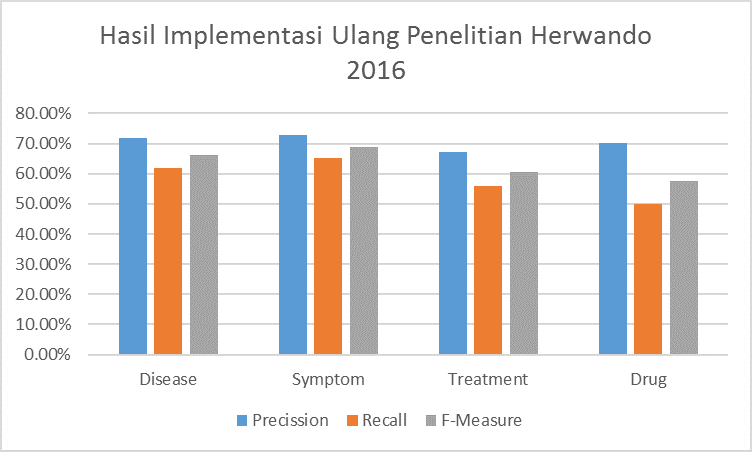
\includegraphics[width=0.85\linewidth]{images/radit}
	\caption{Histogram Metrik Evaluasi dengan Fitur Kata Itu Sendiri}
	\label{fig:radit}
\end{figure}

%-----------------------------------------------------------------------------%
\section{Skenario Eksperimen}
Pada penelitian ini, \saya~melakukan 2 buah skenario utama, yaitu skenario untuk menguji fitur yang memiliki kontribusi untuk meningkatkan akurasi dari setiap eksperimen dan skenario untuk menguji arsitektur RNNs yang \saya~usulkan. Berikut merupakan skenario yang \saya~rancang dalam penelitian ini:
\begin{enumerate}
	\item Skenario untuk menguji fitur\\
	Skenario ini bertujuan untuk mendapatkan kombinasi fitur terbaik sehingga memberikan akurasi terbaik. \Saya~mencoba masing-masing fitur dengan menggunakan model arsitektur LSTM biasa. Apabila penggunaan fitur memberikan hasil yang lebih dari pada hasil eksperimen sebelumnya, fitur tersebut akan dipertahankan untuk eksperimen yang selanjutnya. Skenario ini memiliki 9 sub-skenario, yaitu:
	\begin{enumerate}
		\item Sub-skenario menguji fitur kata itu sendiri
		\item Sub-skenario menguji fitur terbaik sebelumnya ditambahkan fitur kamus
		\item Sub-skenario menguji fitur terbaik sebelumnya ditambahkan fitur stop word
		\item Sub-skenario menguji fitur terbaik sebelumnya ditambahkan fitur POS-Tag
		\item Sub-skenario menguji fitur terbaik sebelumnya ditambahkan fitur Frasa kata
		\item Sub-skenario menguji fitur terbaik sebelumnya dikurang fitur POS-Tag
		\item Sub-skenario menguji fitur terbaik sebelumnya ditambahkan fitur 1 kata sebelum
		\item Sub-skenario menguji fitur terbaik sebelumnya ditambahkan fitur 1 kata sesudah
	\end{enumerate}
	\item Skenario untuk menguji arsitektur RNNs\\
	Skenario ini bertujuan untuk melihat pengaruh arsitektur RNNs pada penelitian ini. \Saya~mencoba kedua arsitektur RNNs yang telah diusulkan sebelumnya dengan menggunakan kombinasi fitur terbaik dari eksperimen di skenario pengujian fitur di atas. Pada skenario ini, terdapat 2 sub-skenario, yaitu:
	\begin{enumerate}
		\item Sub-skenario untuk menguji arsitektur 1 layer
		\item Sub-skenario untuk menguji arsitektur 2 layer
	\end{enumerate}
	
\end{enumerate}

\section{Hasil Eksperimen dan Analisis}
%-----------------------------------------------------------------------------%
Pada bagian ini akan dilaporkan hasil dari ekperimen yang telah \saya~rancang sesuai dengan skenario sebelumnya beserta analisisnya. 
	%-----------------------------------------------------------------------------%
	\subsection{Hasil Ekperimen Pengujian Fitur Beserta Analisis}
	
	Hasil eksperimen ini adalah laporan dari pengujian kombinasi fitur kata itu sendiri, kamus, \textit{stop word}, POS-Tag, frasa kata (frasa kata benda dan kata kerja), 1 kata sebelum,dan 1 kata sesudah.
	  
	\subsubsection{Sub-Eksperimen Menguji Fitur Kata itu Sendiri}
	%-----------------------------------------------------------------------------%
	Merujuk pada penelitian \cite{mujiono2016new}, penelitian tersebut bertujuan untuk mendapatkan \textit{non-handcrafted feature}, yaitu fitur kata itu sendiri dengan menggunakan \textit{tools Word Embedding}. Oleh karena itu, \saya~menguji fitur ini untuk mengetahui pengaruhnya pada program \mer~di penelitian ini. Tabel \ref{table:own1} menampilkan hasil pelabelan otomatis dengan menggunakan fitur kata itu sendiri yang direpresentasikan dengan menggunakan vektor \textit{word embedding}.
	
	\begin{table}
	    \centering
	    \caption{Tabel Hasil Eksperimen dengan Fitur Kata Itu Sendiri}
	    \begin{tabular}{|c|c|c|c|c|}
	      \hline
						      & \textit{Precission} & \f{\f{Recall}} & \f{\f{F-Measure}} \\ \hline
	      \textit{Disease}    & 61.38\%             & 60.42\%        & 60.37\%           \\ \hline
	      \textit{Symptom}    & 57.05\%             & 56.13\%        & 56.19\%           \\ \hline
	      \textit{Treatment}  & 49.92\%             & 47.17\%        & 46.96\%           \\ \hline
	      \textit{Drug}		  & 62.86\%             & 53.32\%        & 57.28\%           \\ \hline
	    \end{tabular}
	    \label{table:own1}
	\end{table}
	
	Pada tabel tersebut, dengan menggunakan fitur kata itu sendiri terlihat bahwa entitas \textit{Disease} memiliki \textit{recall} dan \textit{f-measure} tertinggi, yaitu 60.42\%, dan 60.37\%. Sedangkan entitas \textit{drug} memiliki \textit{precission} tertinggi, yaitu 62.86\%. Grafik \ref{fig:own1} menunjukkan perbandingan \textit{precission}, \textit{recall} dan \textit{f-measure} untuk masing-masing entitas.
	
	\begin{figure}
	  \centering
	  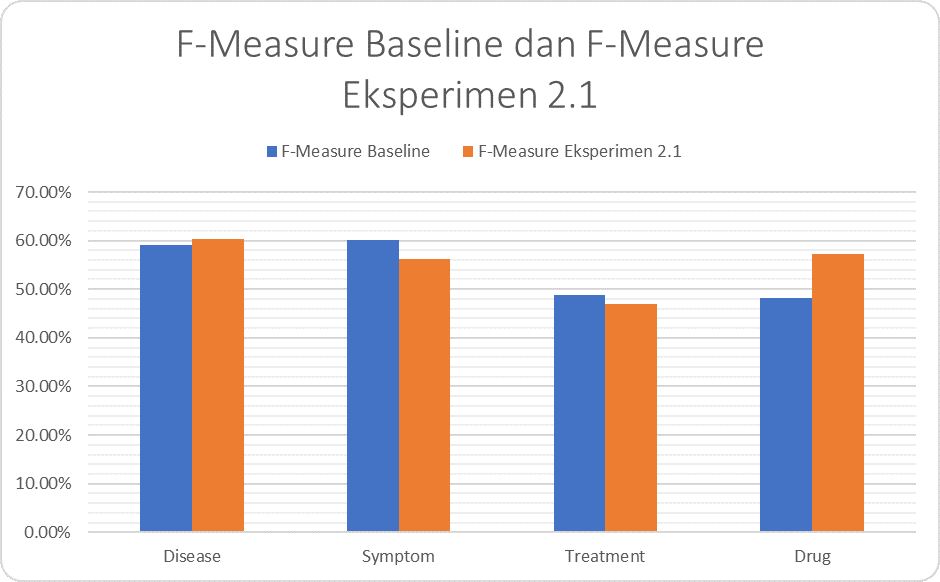
\includegraphics[width=0.85\linewidth]{images/histogram00}
	  \caption{Histogram Metrik Evaluasi dengan Fitur Kata Itu Sendiri}
	  \label{fig:own1}
	\end{figure}

	Pada eksperimen ini, hasil yang dicapai masih lebih kecil apabila dibandingkan dengan hasil yang dicapai \cite{skripsiKakRadit}. Menurut \saya~hal ini terjadi karena pada eksperimen ini hanya menggunakan fitur kata itu sendiri tanpa melibatkan informasi lain seperti pada penelitian yang dilakukan oleh \cite{skripsiKakRadit}. Oleh karena itu perlu adanya informasi lain, misalnya seperti apakah suatu kata terdapat dalam sebuah kamus kesehatan, informasi POS-Tag atau informasi yang lain. Oleh karena itu, \saya~mencoba menggunakan tambahan fitur lain untuk meningkatkan akurasi pada penelitian ini, yaitu pada sub-eksperimen \ref{eks:subeksdict}.
	
	%-----------------------------------------------------------------------------%
	\subsubsection{Sub-Eksperimen Menguji Fitur Terbaik Sebelumnya Ditambahkan Fitur Kamus Kesehatan (\textit{Disease, Symptom, Treatment} dan \textit{Drug})}\label{eks:subeksdict}
	%-----------------------------------------------------------------------------%
	Pada sub-eksperimen ini, \saya~menggunakan tambahan fitur Kamus Kesehatan karena berdasarkan penelitian \cite{skripsiKakRadit} fitur ini memiliki konribusi untuk menambah akurasi pada sistem \mer. Selain itu, menurut \saya, informasi suatu kata terdapat dalam sebuah kamus kesehatan mungkin akan memberikan kontribusi untuk meningkatkan akurasi. Oleh karena itu, \saya~mencoba untuk menambahkan fitur ini ke dalam model RNNs.
	
	Tabel \ref{table:owndict2} merupkan tabel hasil eksperimen yang didapatkan dengan menggunakan fitur ini.
	
	\begin{table}
		\centering
		\caption{Tabel Hasil Eksperimen dengan Fitur Terbaik Sebelumnya Ditambahkan Fitur Kamus Kesehatan}
		\begin{tabular}{|c|c|c|c|c|}
			\hline
			                      & \textit{Precission} & \f{\f{Recall}} & \f{\f{F-Measure}} \\ \hline
			\textit{Disease}      & 67.32\%             & 61.78\%        & 64.10\%           \\ \hline
			\textit{Symptom}      & 60.55\%             & 55.12\%        & 57.41\%           \\ \hline
			\textit{Treatment}    & 52.21\%             & 44.18\%        & 47.02\%           \\ \hline
			\textit{Drug}		  & 59.42\%             & 59.71\%        & 57.90\%           \\ \hline
		\end{tabular}
		\label{table:owndict2}
	\end{table}
	
	Berikut merupakan grafik yang merepresentasikan Tabel \ref{table:owndict2} dalam bentuk histogram.
	
	\begin{figure}
		\centering
		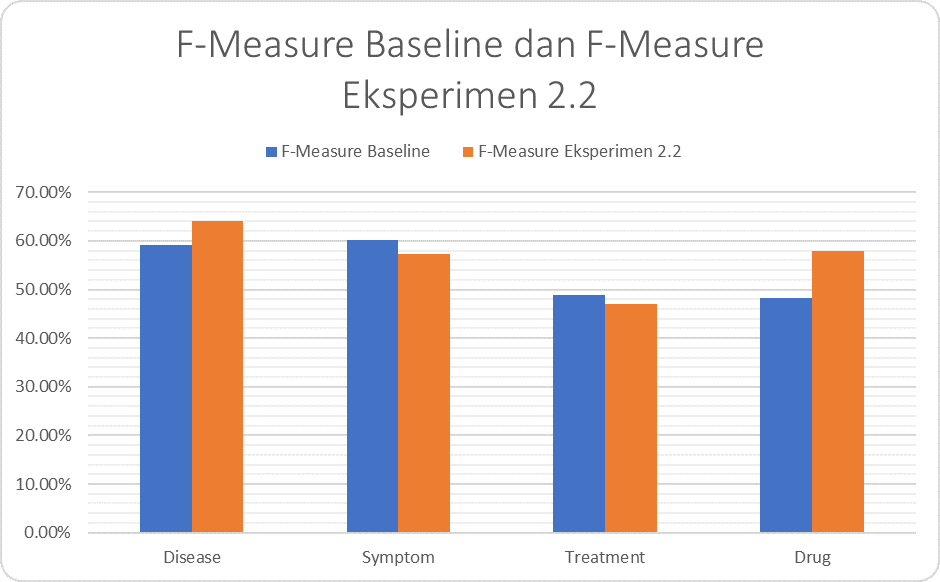
\includegraphics[width=0.85\linewidth]{images/histogram2}
		\caption{Histogram Metrik Evaluasi dengan Fitur Terbaik Sebelumnya Ditambahkan Fitur Kamus Kesehatan}
		\label{fig:owndict2}
	\end{figure}

	Dari tabel dan grafik tersebut, didapatkan informasi bahwa dengan menggunakan tambahan fitur kamus kesehatan terlihat bahwa entitas \textit{Disease} mengalami kenaikan nilai \textit{precission}, \textit{recall}, dan \textit{f-measure}. Selain itu, entitas \textit{Symptom} dan \textit{tratment} mengalami kenaikan nilai \textit{precission} dan \textit{f-measure}. Entitas \textit{drug} mengalami penurunan pada nilai \textit{precission} namun mengalami kenaikan pada nilai \textit{recall} dan \textit{f-measure}-nya. Secara keseluruhan,  Sedangkan entitas \textit{drug} memiliki \textit{precission} tertinggi, yaitu 62.86\%. Grafik \ref{fig:owndict2} menunjukkan perbandingan \textit{precission}, \textit{recall} dan \textit{f-measure} untuk masing-masing entitas.

	Dibandingkan dengan hasil eksperimen \cite{skripsiKakRadit}, hasil yang dicapai pada eksperimen ini masih lebih rendah. Menurut \saya~perlu ada informasi tambahan untuk meningkatkan akurasi. Seperti yang kita ketahui bahwa eksperimen \cite{skripsiKakRadit} tidak hanya menggunakan fitur kata itu sendiri dan kamus kesehatan saja. Oleh karena itu, \saya~mencoba melakukan eksperimen kembali dengan menggunakan tambahan fitur lain pada sub-eksperimen \ref{eks:subekstopword};
	
	%-----------------------------------------------------------------------------%
	\subsubsection{Sub-Eksperimen Menguji Fitur Terbaik Sebelumnya Ditambahkan Fitur Stopword}\label{eks:subekstopword}
	%-----------------------------------------------------------------------------%
	Pada sub-eksperimen ini. \saya~mencoba menambahkan informasi lain berupa fitur yang berisi sebuah kata apakah terdapat di dalam kamus \textit{stop word} atau tidak. \Saya~berpendapat bahwa dengan adanya informasi \textit{stop word}, adanya kesalahan suatu kata tidak berentitas yang dilabeli sebagai kata berentitas oleh model dapat dikurangi.
	
	Rangkuman hasil sub-eksperimen ini dapat dilihat di Tabel \ref{table:owndict3} dan Gambar \ref{fig:owndict3}.
	
	\begin{table}
		\centering
		\caption{Tabel Hasil Eksperimen dengan Fitur Terbaik Sebelumnya Ditambahkan Fitur Stopword}
		\begin{tabular}{|c|c|c|c|c|}
			\hline
							      & \textit{Precission} & \f{\f{Recall}} & \f{\f{F-Measure}} \\ \hline
			\textit{Disease}      & 65.97\%             & 59.81\%        & 62.28\%           \\ \hline
			\textit{Symptom}      & 63.08\%             & 55.20\%        & 58.68\%           \\ \hline
			\textit{Treatment}    & 54.73\%             & 46.27\%        & 49.69\%           \\ \hline
			\textit{Drug}		  & 61.88\%             & 58.99\%        & 59.57\%           \\ \hline
		\end{tabular}
		\label{table:owndict3}
	\end{table}
		
	\begin{figure}
		\centering
		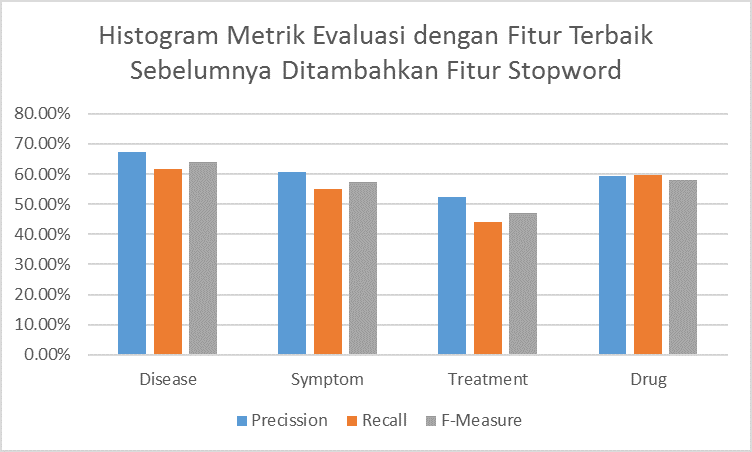
\includegraphics[width=0.85\linewidth]{images/histogram3}
		\caption{Histogram Metrik Evaluasi dengan Fitur Terbaik Sebelumnya Ditambahkan Fitur Stopword}
		\label{fig:owndict3}
	\end{figure}
	
	Dari Tabel \ref{table:owndict3} dan Gambar \ref{fig:owndict3} dapat diamati bahwa secara umum, penggunaan fitur Kamus \textit{Stop Word} dapat meningkatkan \textit{precission, recall,} dan \textit{f-measure}. Untuk lebih detailnya, entitas \textit{disease} mengalami penurunan nilai \textit{precission} dan \textit{f-measure} tetapi mengalami kenaikan nilai \textit{recall}. Entitas \textit{symptom} dan \textit{treatment} mengalami kenaikan untuk nilai \textit{precission, recall} dan \textit{f-measure}. Sedangkan entitas \textit{drug} mengalami kenaikan pada nilai \textit{precission} dan \textit{f-measure} teteapi mengalami penurunan pada nilai \textit{recall}.
	
	Menurut analisis \saya~entitas \textit{symptom} dan \textit{treatment} mengalami kenaikan akurasi karena pada sebagian besar entitas tersebut memiliki susunan kata yang sama dengan kalimat pada umumnya. \textbf{KASIH CONTOH}
	
	Pada sub-eksperimen ini, walaupun secara umum akurasi lebih baik dibandingkan dengan sub-eksperimen sebelumnya, hasil sub-eksperimen ini masih lebih rendah apabila dibandingkan dengan hasil eksperimen \cite{skripsiKakRadit}. Oleh karena \saya~mengusulkan fitur tambahan lain yaitu fitur POS-Tag yang akan dijelaskan pada sub-eksperimen \ref{eks:subekspostag}.
	
	%-----------------------------------------------------------------------------%
	\subsubsection{Sub-Eksperimen Menguji Fitur Terbaik Sebelumnya Ditambahkan Fitur POS-Tag}\label{eks:subekspostag}
	%-----------------------------------------------------------------------------%
	Pada sub-eksperimen ini, \saya~menambahkan informasi baru pada \textit{resource} yang akan digunakan untuk \textit{training} model yang berupa fitur POS-Tag. Sebelumnya fitur ini telah digunakan pada penelitian \cite{abacha2011medical} pada dokumen berbahasa Inggris dan memberikan kontribusi meningkatkan akurasi dari model \mer~yang dibangun. Oleh karena itu pada eksperimen ini \saya~mencoba menggunakan fitur tersebut dan ingin mengetahui apakah fitur POS-Tag memiliki kontribusi untuk meningkatkan akurasi pada \mer~dengan dokumen berbahasa Indonesia. 
	
	Rangkuman hasil sub-eksperimen ini dapat dilihat pada Tabel \ref{table:owndict4} dan Gambar \ref{fig:owndict4}.
	
	\begin{table}
		\centering
		\caption{Tabel Hasil Eksperimen dengan Fitur Terbaik Sebelumnya Ditambahkan Fitur POS-Tag}
		\begin{tabular}{|c|c|c|c|c|}
			\hline
								  & \textit{Precission} & \f{\f{Recall}} & \f{\f{F-Measure}} \\ \hline
			\textit{Disease}      & 69.10\%             & 58.67\%        & 63.22\%           \\ \hline
			\textit{Symptom}      & 61.09\%             & 54.43\%        & 57.00\%           \\ \hline
			\textit{Treatment}    & 59.73\%             & 44.10\%        & 49.87\%           \\ \hline
			\textit{Drug}		  & 62.00\%             & 55.74\%        & 57.87\%           \\ \hline
		\end{tabular}
		\label{table:owndict4}
	\end{table}
	
	\begin{figure}
		\centering
		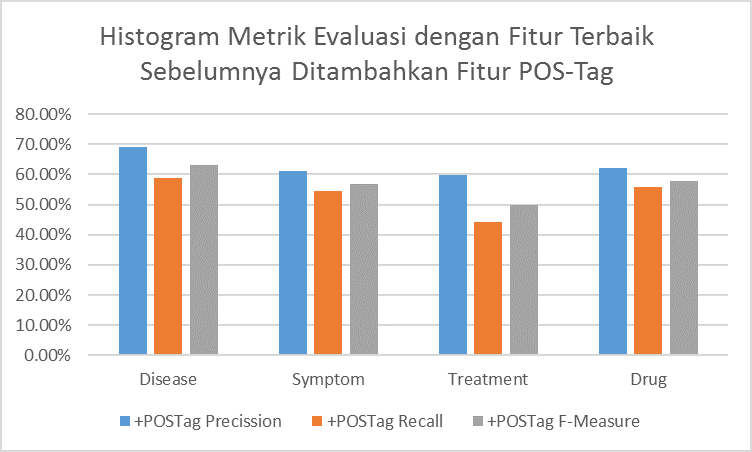
\includegraphics[width=0.85\linewidth]{images/histogram4}
		\caption{Histogram Metrik Evaluasi dengan Fitur Terbaik Sebelumnya Ditambahkan Fitur POS-Tag}
		\label{fig:owndict4}
	\end{figure}
	
	Dari tabel dan grafik di atas, entitas \textit{disease} dan \textit{treatment} memiliki nilai \textit{precission} dan \textit{f-measure} yang meningkat, tetapi dengan nilai \textit{recall} yang turun. Untuk entitas \textit{symptom}, nilai \textit{precission, recall}, dan \textit{f-measure} mengalami penurunan. Sedangkan entitas \textit{drug} mengalami kenaikan hanya pada \textit{precission}-nya saja. Hal ini terjadi karena model POS-Tagger yang digunakan menghasilkan tag yang terkadang tidak konsisten. Sebagai contoh, \textbf{BERI CONTOH}. Selain itu, fitur POS-Tag juga tidak dapat membedakan entitas obat, nama penyakit dan nama orang. Sebagai contoh, \textbf{KASIH CONTOH}. Kemudian untuk POS-Tag pada entitas \textit{treatment}juga tidak dapat dibedakan dengan POS-Tag pada kalimat yang lebih umum. Sebagai contoh \textbf{KASIH CONTOH}.
	
	Oleh karena itu pada sub-eksperimen selanjutnya, \saya~mencoba menambahkan fitur lain yang lebih spesifik dibandingkan dengan fitur POS-Tag, yaitu fitur Frasa Kata. Penjelasan lebih lanjut akan dibahas pada sub-eksperimen \ref{eks:subeksfrasa}.
	
	%-----------------------------------------------------------------------------%
	\subsubsection{Sub-Eksperimen Menguji Fitur Terbaik Sebelumnya Ditambahkan Fitur Frasa Kata}\label{eks:subeksfrasa}
	%-----------------------------------------------------------------------------%
	Pada sub-eksperimen ini \saya~menambahkan fitur baru yaitu fitur Frasa Kata. Seperti yang telah dijelaskan pada Bab 3, entitas \textit{symptom} dan \textit{treatment} diharapkan akan lebih mudah dikenali karena pada umumnya merupakan frasa kata kerja. Sedangkan entitas \textit{disease} dan \textit{drug} diharapkan juga akan lebih mudah dikenali karena pada umumnya merupakan frasa kata benda. Alasan lain yaitu karena pada umumnya entitas yang akan dikenali pada penelitian ini merupakan frasa kata, hal ini dibuktikan dengan \textbf{KASIH BUKTI}.
	
	Rangkuman hasil sub-eksperimen ini dapat dilihat pada Tabel \ref{table:owndict4} dan Gambar \ref{fig:owndict4}.
	
	\begin{table}
		\centering
		\caption{Rangkuman Hasil Eksperimen dengan Fitur Terbaik Sebelumnya Ditambahkan Fitur Frasa Kata}
		\begin{tabular}{|c|c|c|c|c|}
			\hline
			                      & \textit{Precission} & \f{\f{Recall}} & \f{\f{F-Measure}} \\ \hline
			\textit{Disease}      & 67.49\%             & 61.56\%        & 63.81\%           \\ \hline
			\textit{Symptom}      & 62.89\%             & 52.27\%        & 56.72\%           \\ \hline
			\textit{Treatment}    & 54.87\%             & 44.92\%        & 49.06\%           \\ \hline
			\textit{Drug}		  & 59.77\%             & 53.37\%        & 55.66\%           \\ \hline
		\end{tabular}
		\label{table:owndict5}
	\end{table}

	\begin{figure}
		\centering
		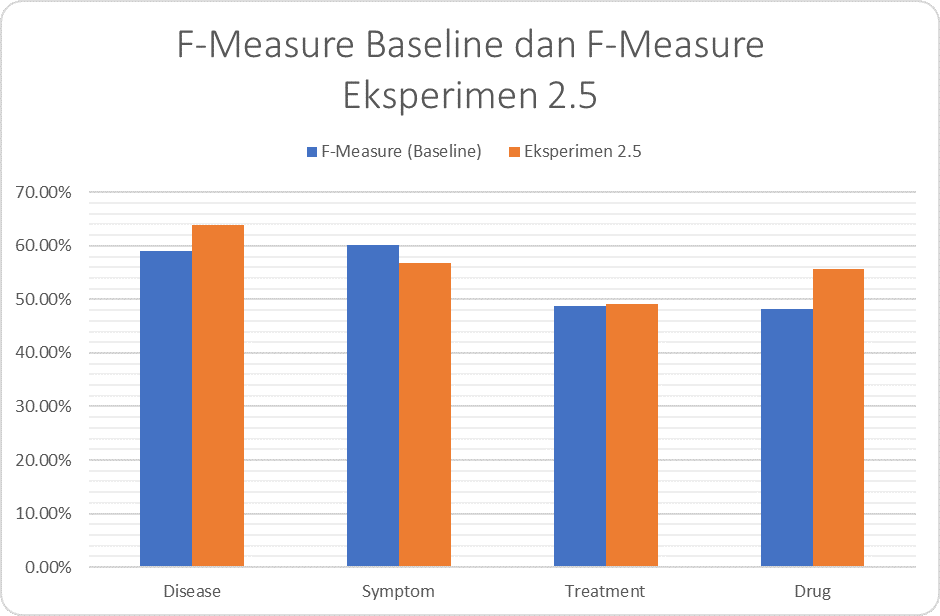
\includegraphics[width=0.85\linewidth]{images/histogram5}
		\caption{Histogram Metrik Evaluasi dengan Fitur Terbaik Sebelumnya Ditambahkan Fitur Frasa Kata}
		\label{fig:owndict5}
	\end{figure}

	Dari tabel dan grafik di atas, entitas \textit{drug} mengalami penurunan untuk nilai \textit{precission, recall} dan \textit{f-measure}. Selain itu, entitas \textit{disease} mengalami penurunan pada nilai \textit{precission} tetapi mengalami kenaikan pada nilai \textit{recall} dan \textit{f-measure}. Entitas \textit{symptom} mengalami kenaikan pada nilai \textit{precission} tetapi mengalami penurunan pada nilai \textit{recall} dan \textit{f-measure}. Sedangkan pada entitas \textit{treatment}, terjadi kenaikan nilai \textit{recall} tetapi nilai \textit{precission} dan \textit{f-measure} mengalami penurunan. 
	
	Dari hasil eksperimen ini, menurut \saya~hal ini terjadi karena informasi frasa bersifat redundan apabila bergabung dengan fitur POS-Tag. Pada fitur POS-Tag, tidak ada perbedaan antara kata yang merupakan frasa maupun kata yang bukan frasa. Padahal, mayoritas entitas merupakan frasa. Oleh karena itu, pada sub-eksperimen \ref{eks:subeksminpostag}, penulis menghilangkan fitur POS-Tag dan tetap mempertahankan fitur Frasa Kata untuk mengetahui hal tersebut. 
	
	%-----------------------------------------------------------------------------%
	\subsubsection{Sub-Eksperimen Menguji Fitur Terbaik Sebelumnya Dikurangi Fitur POS-Tag}\label{eks:subeksminpostag}
	%-----------------------------------------------------------------------------%
	Pada sub-eksperimen ini \saya~menghilangkan fitur POS-Tag berdasarkan hasil dan analisis pada sub-eksperimen \ref{subeksfrasa}. Rangkuman hasil sub-eksperimen ini dapat dilihat pada Tabel \ref{table:owndict6} dan Gambar \ref{fig:owndict6}.
	
	\begin{table}
		\centering
		\caption{Rangkuman Hasil Eksperimen dengan Fitur Terbaik Sebelumnya Dikurangi Fitur POS-Tag}
		\begin{tabular}{|c|c|c|c|c|}
			\hline
			                      & \textit{Precission} & \f{\f{Recall}} & \f{\f{F-Measure}} \\ \hline
			\textit{Disease}      & 68.67\%             & 61.80\%        & 64.78\%           \\ \hline
			\textit{Symptom}      & 63.79\%             & 56.10\%        & 59.23\%           \\ \hline
			\textit{Treatment}    & 54.47\%             & 46.72\%        & 49.58\%           \\ \hline
			\textit{Drug}		  & 60.08\%             & 56.70\%        & 57.00\%           \\ \hline
		\end{tabular}
		\label{table:owndict6}
	\end{table}
	
	\begin{figure}
		\centering
		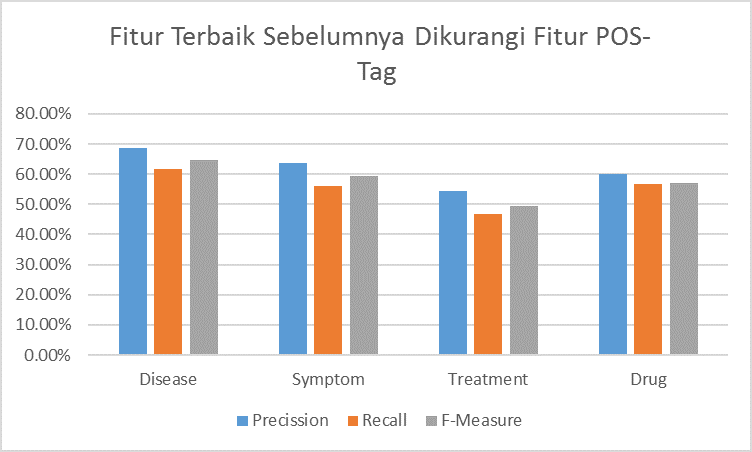
\includegraphics[width=0.85\linewidth]{images/histogram6}
		\caption{Histogram Metrik Evaluasi dengan Fitur Terbaik Sebelumnya Dikurangi Fitur POS-Tag}
		\label{fig:owndict6}
	\end{figure}
	
	Dari Tabel \ref{table:owndict6} dan Gambar \ref{fig:owndict6}, terlihat bahwa semua entitas (\textit{disease, symptom, treatment,}) dan \textit{drug} mengalami kenaikan pada nilai \textit{precission, recall,} dan \textit{f-measure}. Seperti yang telah dijelaskan pada sub-eksperimen \ref{eks:subeksfrasa}, penggabunagn fitur POS-Tag dan Frasa akan memberikan hasil yang lebih rendah. Oleh karena itu, sebaiknya fitur POS-Tag tidak digabung dengan fitur Frasa. Selain itu, \saya~lebih memilih fitur Frasa untuk dipertahankan karena fitur ini lebih diskriminatif dibandingkan dengan fitur POS-Tag, dengan melihat bahwa mayoritas kata berentitas merupakan frasa.
	
	Walaupun pada sub-eksperimen ini hasil yang dicapai lebih baik dari sub-eksperimen sebelumnya, hasilnya tetap lebih rendah dari hasil eksperimen \cite{skripsiKakRadit}. Oleh karena itu \saya~mencoba fitur yang lain, yaitu fitur Kata Sebelum. Untuk penjelasan lebih lanjut akan dibahas pada sub-eksperimen \ref{eks:subekswbef1}.
	
	%-----------------------------------------------------------------------------%
	\subsubsection{Sub-Eksperimen Menguji Fitur Terbaik Sebelumnya Ditambahkan Fitur 1 Kata Sebelum}\label{eks:subekswbef1}
	%-----------------------------------------------------------------------------%
	Pada sub-eksperimen ini \saya~menambahkan fitur baru yaitu fitur 1 Kata Sebelum. Fitur ini digunakan pada penelitian \cite{skripsiKakRadit} yang juga berkontribusi memberikan hasil terbaik pada penelitiannya. Menurut \saya, ada beberapa entitas yang akan lebih mudah diketahui apabila diketahui kata sebelumnya. Misalnya kata "masuk angin", apabila hanya diberikan informasi kata "angin" tanpa kata "masuk", akan lebih sulit menentukan kata tersebut bagian dari suatu entitas \textit{disease} atau bukan. Oleh karena itu, pada sub-eksperimen ini saya mencoba menambahkan fitur tersebut.
	
	Rangkuman hasil sub-eksperimen ini dapat dilihat pada Tabel \ref{table:owndict7} dan Gambar \ref{fig:owndict7}.
	
	\begin{table}
		\centering
		\caption{Rangkuman Hasil Eksperimen dengan Fitur Terbaik Sebelumnya Ditambahkan Fitur 1 Kata Sebelum}
		\begin{tabular}{|c|c|c|c|c|}
			\hline
		                          & \textit{Precission} & \f{\f{Recall}} & \f{\f{F-Measure}} \\ \hline
			\textit{Disease}      & 69.49\%             & 61.60\%        & 64.68\%           \\ \hline
			\textit{Symptom}      & 64.78\%             & 57.15\%        & 60.23\%           \\ \hline
			\textit{Treatment}    & 56.58\%             & 44.71\%        & 49.54\%           \\ \hline
			\textit{Drug}		  & 62.22\%             & 57.28\%        & 58.76\%           \\ \hline
		\end{tabular}
		\label{table:owndict7}
	\end{table}
	
	\begin{figure}
		\centering
		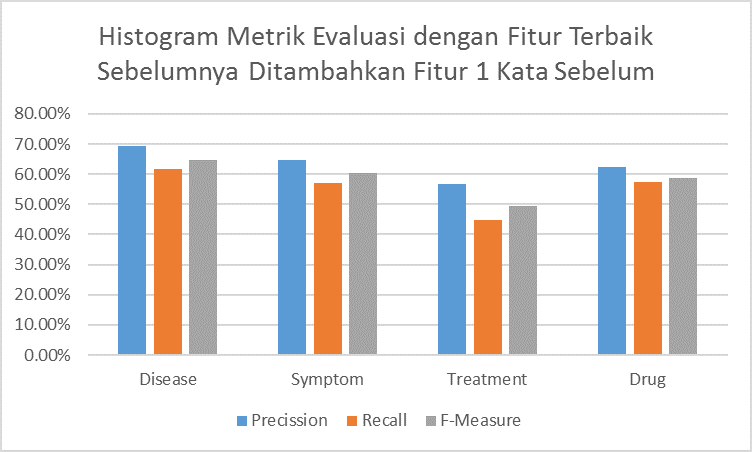
\includegraphics[width=0.85\linewidth]{images/histogram7}
		\caption{Histogram Metrik Evaluasi dengan Fitur Terbaik Sebelumnya Ditambahkan Fitur 1 Kata Sebelum}
		\label{fig:owndict7}
	\end{figure}
	
	Melihat pada Tabel \ref{table:owndict7} dan Gambar \ref{fig:owndict7}, dapat diketahui bahwa entitas \textit{disease} dan \textit{treatment} mengalami kenaikan pada nilai \textit{precission}, tetapi mengalami penurunan pada nilai \textit{recall} dan \textit{f-measure}. Sedangkan entitas \textit{symptom} dan \textit{drug} mengalami kenaikan pada nilai \textit{precission, recall,} dan \textit{f-measure}.
	
	Hasil sub-eksperimen ini masih lebih rendah dibandingkan dengan hasil eksperimen \cite{skripsiKakRadit}. Oleh karena itu, \saya~mencoba menambahkan fitur yang lain yaitu fitur 1 Kata Sesudah, yang akan dibahas lebih lanjut pada sub-eksperimen \ref{eks:subekswaf1}.
	
	
	%-----------------------------------------------------------------------------%
	\subsubsection{Sub-Eksperimen Menguji Fitur Terbaik Sebelumnya Ditambahkan Fitur 1 Kata Sesudah}\label{eks:subekswaf1}
	%-----------------------------------------------------------------------------%
	Pada sub-eksperimen ini \saya~menambahkan fitur lain yaitu fitur 1 Kata Setelah. Hal ini karena ada beberapa kasus yang mana apabila suatu kata merupakan sebuah entitas, akan lebih mudah dikenali apabila melihat kata atau konteks setelahnya. Sama seperti contoh pada Fitur 1 Kata Sebelum, misal diberikan kata "masuk angin", apabila hanya diberikan informasi "masuk" tanpa "angin", akan lebih sulit mengenali apakah kata tersebut termasuk entitas \textit{disease} atau bukan. Selain itu, fitur ini juga dapat membedakan kata berentitas dengan kata yang bukan, misalnya kata "masuk angin" dengan "masuk rumah". Apabila informasi pada saat tersebut hanya diberikan kata "masuk" saja tanpa kata setelahnya, akan lebih sulit mengenali kata tersebut termasuk kata berentitas atau bukan.
	
	Rangkuman hasil sub-eksperimen ini dapat dilihat pada Tabel \ref{table:owndict8} dan Gambar \ref{fig:owndict8}.
	
	\begin{table}
		\centering
		\caption{Rangkuman Hasil Eksperimen dengan Fitur Terbaik Sebelumnya Ditambahkan Fitur 1 Kata Sesudah}
		\begin{tabular}{|c|c|c|c|c|}
			\hline
			& \textit{Precission} & \f{\f{Recall}} & \f{\f{F-Measure}} \\ \hline
			\textit{Disease}      & 70.68\%             & 66.18\%        & 68.17\%           \\ \hline
			\textit{Symptom}      & 64.16\%             & 59.55\%        & 61.42\%           \\ \hline
			\textit{Treatment}    & 61.02\%             & 51.13\%        & 54.03\%           \\ \hline
			\textit{Drug}		  & 70.85\%             & 70.33\%        & 69.82\%           \\ \hline
		\end{tabular}
		\label{table:owndict8}
	\end{table}
	
	\begin{figure}
		\centering
		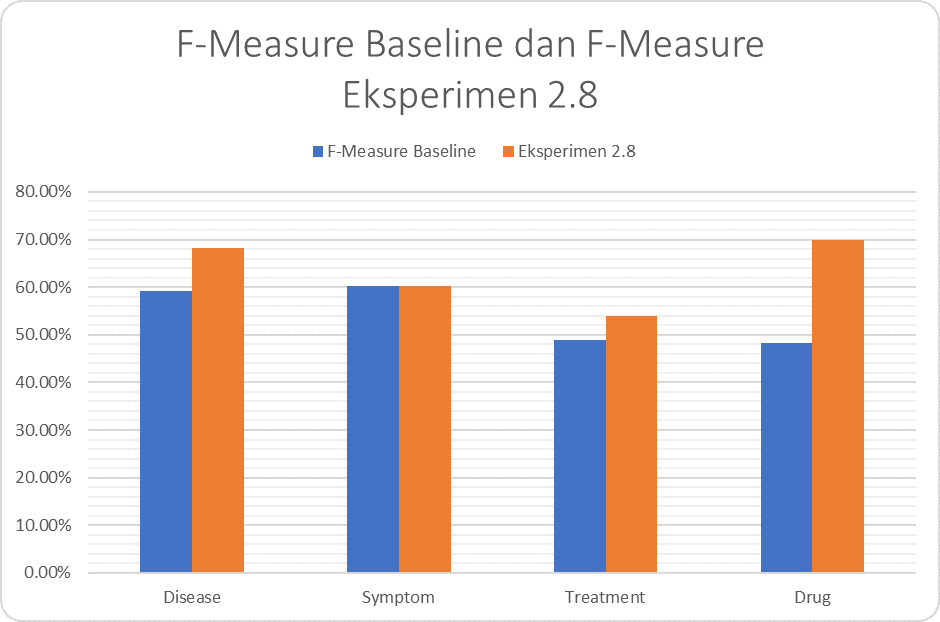
\includegraphics[width=0.85\linewidth]{images/histogram8}
		\caption{Histogram Metrik Evaluasi dengan Fitur Terbaik Sebelumnya Ditambahkan Fitur 1 Kata Sesudah}
		\label{fig:owndict8}
	\end{figure}
	
	Melihat pada Tabel \ref{table:owndict8} dan Gambar \ref{fig:owndict8}, dapat diketahui bahwa hanya entitas \textit{symptom} yang mengalami penurunan tetapi nilai \textit{recall} dan \textit{f-measure}-nya naik. Sedangkan entitas lain mengalami kenaikan pada nilai \textit{precission, recall} dan \textit{f-measure}. Akan tetapi hasil sub-eksperimen ini masih lebih rendah dibandingkan dengan hasil eksperimen \cite{skripsiKakRadit}. Oleh karena itu, setelah \saya~mencoba kemungkinan fitur yang memberikan kontribusi dalam penelitian ini, \penulis~mencoba arsitektur untuk model RNNs yang lain. Penjelasan lebih lanjut akan dibahas pada eksperimen \ref{eks:eks2}.
	
	
	
  %-----------------------------------------------------------------------------%
  
  
    \subsection{Hasil Ekperimen Pengujian Arsitektur RNNs}\label{eks:eks2}
    
    Pada eksperimen ini, \saya~mencoba dua buah arsitektur RNNs yang telah \saya~usulkan pada Bab3 yaitu RNNs dengan 1 layer dan RNNs dengan 2 layer. Fitur yang digunakan dalam pengujian ini yaitu kombinasi fitur yang menghasilkan akurasi terbaik pada eksperimen pertama, yaitu fitur Kata itu Sendiri, Kamus Kesehatan, \textit{Stop Word}, Frasa Kata, 1 Kata Sebelum dan 1 Kata Sesudah.
    
    \subsubsection{Sub-Eksperimen Menguji Arsitektur RNNs 1 Layer}\label{eks2:subeksrnn1}
    %-----------------------------------------------------------------------------%
    Pada sub-eksperimen ini, \saya~menggunakan struktur RNNs yang mana semua fitur digabung menjadi satu dalam sebuah \textit{timestep}.
    Artinya fitur-fitur yang berbeda tersebut akan digabung atau di-\textit{concat} menjadi sebuah vektor yang akan menjadi \textit{input} bagi RNNs ini. RNNs inilah yang digunakan pada eksperimen pertama, sehingga hasilnya sama dengan sub-eksperimen \ref{eks:subekswaf1}.
    
    \begin{table}
    	\centering
    	\caption{Rangkuman Hasil Eksperimen dengan Arsitektur RNNs 1 Layer}
    	\begin{tabular}{|c|c|c|c|c|}
    		\hline
    		& \textit{Precission} & \f{\f{Recall}} & \f{\f{F-Measure}} \\ \hline
    		\textit{Disease}      & 70.68\%             & 66.18\%        & 68.17\%           \\ \hline
    		\textit{Symptom}      & 64.16\%             & 59.55\%        & 61.42\%           \\ \hline
    		\textit{Treatment}    & 61.02\%             & 51.13\%        & 54.03\%           \\ \hline
    		\textit{Drug}		  & 70.85\%             & 70.33\%        & 69.82\%           \\ \hline
    	\end{tabular}
    	\label{table:owndict9}
    \end{table}
    
    \begin{figure}
    	\centering
    	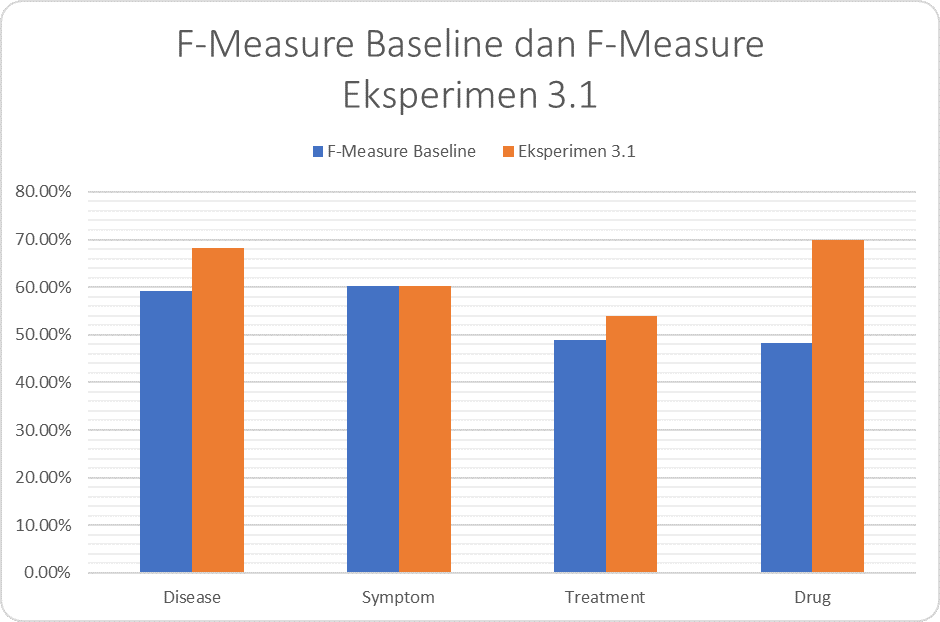
\includegraphics[width=0.85\linewidth]{images/histogram9}
    	\caption{Histogram Metrik Evaluasi dengan Arsitektur RNNs 1 Layer}
    	\label{fig:owndict9}
    \end{figure}
    
    Pada eksperimen ini, hasil yang dicapai masih lebih kecil apabila dibandingkan dengan hasil yang dicapai \cite{skripsiKakRadit}. Menurut \saya~hal ini terjadi karena informasi fitur yang berbeda-beda dijadikan satu, sehingga ada kemungkinan hilangnya informasi dari masing-masing fitur tersebut. Oleh karena itu, untuk mengatasi permasalahan tersebut \saya~mengusulkan arsitektur yang mana masing-masng kelompok fitur yang berbeda dipisahkan dan menjadi \textit{input} bagi masing-masing LSTMs. Untuk penjelasan eksperimen ini akan dijelaskan pada sub-eksperimen \ref{eks2:subeksrnn2}
    
    
    \subsubsection{Sub-Eksperimen Menguji Arsitektur RNNs 2 Layer}\label{eks2:subeksrnn2}
    %-----------------------------------------------------------------------------%
    Pada sub-eksperimen sebelumnya, fitur-fitur yang berbeda digabung menjadi satu, sehingga ada kemungkinan hilangnya informasi dari fitur tersebut. Oleh karena itu, \saya~mengusulkan adanya layer tambahan setelah masing-masing fitur tersebut masuk ke dalam model. \Saya~mengusulkan bahwa masing-masing kelompok fitur menjadi \textit{input} RNNs secara terpisah. Setelah masuk di RNNs, \textit{output} dari masing-masing RNNs tersebut di-\textit{merge} ke dalam sebuah layer, lalu masuk kembali ke RNNs untuk melihat konteks fitur-fitur sebelumnya. Dengan diusulkannya arsitektur RNNs ini \saya~berharap bahwa masing-masing fitur terjaga informasinya dan tidak terganggu dengan informasi lain.
    
    Rangkuman hasil sub-eksperimen ini dapat dilihat pada Tabel \ref{table:owndict10} dan Gambar \ref{fig:owndict10}.
    
    \begin{table}
    	\centering
    	\caption{Rangkuman Hasil Eksperimen dengan Arsitektur RNNs 2 Layer}
    	\begin{tabular}{|c|c|c|c|c|}
    		\hline
    		& \textit{Precission} & \f{\f{Recall}} & \f{\f{F-Measure}} \\ \hline
    		\textit{Disease}      & 67.47\%             & 67.19\%        & 66.31\%           \\ \hline
    		\textit{Symptom}      & 64.90\%             & 60.63\%        & 62.13\%           \\ \hline
    		\textit{Treatment}    & 63.92\%             & 53.13\%        & 56.51\%           \\ \hline
    		\textit{Drug}		  & 66.39\%             & 62.33\%        & 63.61\%           \\ \hline
    	\end{tabular}
    	\label{table:owndict10}
    \end{table}
    
    \begin{figure}
    	\centering
    	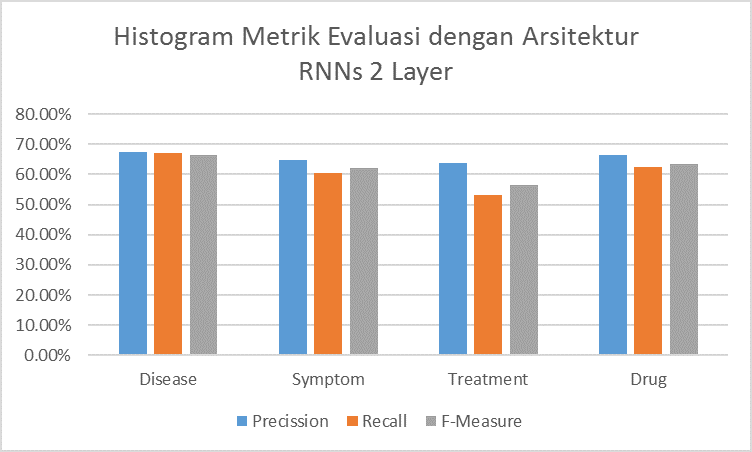
\includegraphics[width=0.85\linewidth]{images/histogramrnnv2}
    	\caption{Histogram Metrik Evaluasi dengan Arsitektur RNNs 2 Layer}
    	\label{fig:owndict10}
    \end{figure}
%!TEX root = skripsi.tex
%-----------------------------------------------------------------------------%
\chapter{\babEnam}
%-----------------------------------------------------------------------------%

%-----------------------------------------------------------------------------%
\section{Kesimpulan}
%-----------------------------------------------------------------------------%
Penelitian ini bertujuan untuk membangun sistem yang mampu melakukan ekstraksi entitas kesehatan dari forum \textit{online} secara otomatis. Data yang digunakan bersumber dari \textit{post} pada forum kesehatan \textit{online} yang telah didapatkan oleh \cite{skripsiKakRadit} dan \saya. Fitur yang digunakan pada penelitian ini yaitu fitur kata itu sendiri, kamus kesehatan, \textit{stop word}, POS-Tag, frasa kata,  1 kata sebelum dan 1 kata sesudah. Penelitian ini juga menggunakan dua arsitektur RNNs yang diusulkan, yaitu LSTMs dengan 1 layer dan LSTMs dengan 2 layer dengan multi-\textit{input}.

Terkait dengan rumusan masalah pertama, setelah dilakukan penelitian secara garis besar didapatkan kesimpulan bahwa model RNNs yang dihasilkan mampu memberikan performa yang lebih baik dibandingkan dengan model CRF (\textit{baseline}) pada penelitian \cite{skripsiKakRadit}. Dari penggunaan fitur kata itu sendiri saja, model RNNs sudah memberikan performa yang lebih baik dengan nilai \textit{F-Measure} dan \textit{recall} yang lebih tinggi.

Terkait dengan rumusan masalah kedua, didapatkan kesimpulan lain bahwa fitur kata itu sendiri, kamus kesehatan, \textit{stop word}, frasa Kata,  1 kata sebelum dan 1 kata sesudah memberikan hasil yang terbaik, yaitu dengan rata-rata \textit{f-measure} $ 63.06\% $ (\textit{disease} $ 68.17\% $, \textit{symptom} $ 61.42\% $, \textit{treatment} $ 68.17\% $ dan \textit{drug} $ 68.17\% $).

Dua arsitektur yang diusulkan memiliki kelebihan masing-masing. Untuk arsitektur LSTMs dengan 1 layer, \textit{f-measure} sama dengan percobaan untuk mendapatkan fitur terbaik, karena eksperimen tersebut menggunakn arsitektur LSTMs yang sama. Sedangkan untuk arsitektur kedua (LSTMs 2 layer), rata-rata \textit{f-measure} yang didapatkan adalah $ 62.14\% $. LSTMs pertama memiliki nilai \textit{f-measure} pada entitas \textit{disease} dan \textit{drug} yang lebih bagus, yaitu masing-masing $ 68.17\% $ dan $ 69.82\% $. Sedangkan LSTMs kedua memiliki nilai \textit{f-measure} pada entitas \textit{symptom} $ 62.13\% $ dan \textit{treatment} $ 56.51\% $. Namun, apabila dilihat dari waktu komputasi, LSTMs pertama lebih baik dibandingkan LSTMs kedua.

LSTMs pertama tidak bisa dikatakan lebih baik dibandingkan LSTMs kedua dan begitu pula sebaliknya, karena hasil yang diperoleh mengatakan bahwa masing-masing arsitektur memiliki hasil yang lebih baik di beberapa macam entitas. Namun, arsitektur ini mampu memberikan hasil yang lebih baik dari hasil penelitian \cite{skripsiKakRadit}. Hal ini akan menarik apabila \textit{resource} semakin diperbesar, apakah tetap LSTMs 1 layer lebih baik, karena LSTMs 2 layer memiliki parameter lebih banyak, sehingga mampu menyimpan informasi yang lebih besar.

%-----------------------------------------------------------------------------%
\section{Saran}
%-----------------------------------------------------------------------------%
Setelah melakukan eksperimen dan menganalisis hasilnya, ada beberapa saran untuk penelitian selanjutnya, antara lain sebagai berikut.

\begin{enumerate}
  \item Penelitian ini hanya menggunakan 309 \textit{post} forum kesehatan \textit{online} sehingga perlu penambahan data \textit{training} dan \textit{testing} mengingat \textit{deep learning} membutuhkan data yang besar dalam melakukan \textit{training} untuk mendapatkan model yang baik.
  
  \item Terdapat beberapa parameter bebas seperti dalam pembuatan model \textit{word embedding} yaitu panjang \textit{window} dan \textit{vector}. Hal ini bisa menjadi bahan penelitian lanjutan untuk mendapatkan panjang \textit{window} dan \textit{vector} yang tepat supaya model mampu memberikan akurasi yang lebih baik.
  
  \item Dalam menentukan label entitas, \saya~tidak mempertimbangkan konteks kalimat yang berada di sekitarnya. Padahal kalimat di sekitarnya akan memberikan informasi lebih terkait hubungan antar entitas. Misalnya pada kalimat pertama dokter menjelaskan penyakit yang dialami. Pada kalimat selanjutnya dokter tersebut menjelaskan cara penyembuhan dari penyakit tersebut. Oleh karena itu, \saya~menyarankan untuk mempertimbangkan fitur konteks kalimat pada penelitian selanjutnya.
  

  \item Perlu dibuat korpus dengan jumlah masing-masing entitas yang seimbang, sehingga hasil yang diberikan tidak bias.
  
  \item Sebaiknya, pelabelan dokumen secara manual melibatkan pihak yang ahli di bidangnya (dalam hal ini dokter, perawat, apoteker, atau mahasiswa di bidang kesehatan) supaya label yang diberikan lebih tepat.
  
  \item Sama seperti pada penelitian \cite{skripsiKakRadit}, sebaiknya dibuat model POS-Tagger yang khusus di bidang kesehatan, sehingga pemberian tag pada dokumen kesehatan lebih tepat.

\end{enumerate}

%\printbibliography
%
% Daftar Pustaka
%\include{pustaka}
%biblama (bukan biblatex)
\bibliography{skripsi}{}
%\bibliography{references}{}
%biblama (bukan biblatex)
\bibliographystyle{apalikerd}
%\bibliographystyle{ieeetr} 

%
% Lampiran 
%
\begin{appendix}
	%!TEX root = skripsi.tex
%
% @author  Andreas Febrian
% @version 1.00 
% 
% Hanya sebuah pembatas bertuliskan LAMPIRAN ditengah halaman. 
% 

\begin{titlepage}
	\centering 
	\vspace*{6cm}
	\noindent \Huge{LAMPIRAN}
	\addChapter{LAMPIRAN}
\end{titlepage}
 	%!TEX root = skripsi.tex
\section{PART OF SPEECH TAG BAHASA INDONESIA}
\begin{longtable}{|c|c|p{.50\textwidth}|p{.40\textwidth}|}
	\caption{Daftar POSTAG Bahasa Indonesia}\label{lampiran:postag}\\
	% header and footer information
	\hline
	\multicolumn{1}{|c|}{\textbf{No}} & \multicolumn{1}{c|}{\textbf{Tag}} & \multicolumn{1}{c|}{\textbf{Deskripsi}} & \multicolumn{1}{c|}{Contoh} \\
	\hline
	\endhead
	\hline
	\endfoot
	1 & CC & Konjungtor koordinatif menghubungkan dua satuan bahasa atau lebih yang sederajat (kata dengan kata; frasa dengan frasa; atau klausa dengan klausa) yang masing-masing mempunyai kedudukan yang setara dalam struktur kalimat. & dan;tetapi;atau \\ \hline
	2 & CD & Numeralia kardinal; yaitu numeralia yang menjadi jawaban atas pertanyaan "Berapa?" & dua; juta; enam; 7916; sepertiga; 0;025; 0;525; banyak; kedua; ribuan; 2007; 25 \\ \hline
	3 & OD & Numeralia ordinal menyatakan urutan dan menjadi jawaban atas pertanyaan "Yang keberapa?" & ketiga; ke-4; pertama \\ \hline
	4 & DT & Artikel bertugas membatasi makna nomina. & para; sang; si \\ \hline
	5 & FW & Kata bahasa asing adalah kata yang berasal dari bahasa asing yang belum diserap ke dalam bahasa Indonesia. Pada dasarnya; kata bahasa asing adalah katayang tidak terdapat di dalam kamus bahasa Indonesia. &  \\ \hline
	6 & IN & Preposisi menghubungkan kata atau frasa dengan konstituen di depan preposisi tersebut sehingga terbentuk frasa preposisional. & dalam; dengan; di; ke; oleh; pada; untuk \\ \hline
	7 & JJ & Adjektiva adalah kata yang memberikan keterangan yang lebih khusus tentang sesuatu yang dinyatakan oleh nomina dalam kalimat. & bersih; panjang; hitam; lama; jauh; marah; suram; nasional; bulat \\ \hline
	8 & MD & Verba modal dan verba bantu. & boleh; harus; sudah; mesti; perlu \\ \hline
	9 & NEG & Kata ingkar. & tidak; belum; jangan \\ \hline
	10 & NN & Nomina; yaitu kata yang mengacu pada manusia; binatang; benda; konsep; atau pengertian & monyet; bawah; sekarang; rupiah \\ \hline
	11 & NNP & Proper noun adalah nama spesifik dari seseorang; sesuatu; atau sebuah tempat. & Boediono; Laut Jawa; Indonesia; India; Malaysia; Bank Mandiri; BBKP; Januari; Senin; Idul Fitri; Piala Dunia; Liga Primer; Lord of the Rings: The Return of the King \\ \hline
	12 & NND & Penggolong menempatkan nomina ke dalam sebuah kelompok tertentu dalam jumlah tertentu; misalnya orang dalam dua orang prajurit. & orang; ton; helai; lembar \\ \hline
	13 & PR & Demonstrativa atau pronomina penunjuk. & ini; itu; sini; situ \\ \hline
	14 & PRP & Pronomina persona; yaitu pronomina yang dipakai untuk mengacu pada orang. & saya; kami; kita; kamu; kalian; dia; mereka \\ \hline
	15 & RB & Adverbia; atau disebut juga kata keterangan. & sangat; hanya; justru; niscaya; segera \\ \hline
	16 & RP & Dalam penelitian ini; POS tag RP menandai partikel penegas; yaitu partikel yang digunakan untuk menegaskan kalimat interogatif; imperatif; atau deklaratif. & pun; -lah; -kah \\ \hline
	17 & SC & Konjungtor subordinatif menghubungkan dua klausa atau lebih dan salah satu dari klausa-klausa tersebut merupakan klausa subordinatif. & sejak; jika; seandainya; supaya; meski; seolah-olah; sebab; maka; tanpa; dengan; bahwa; yang; lebih; daripada; semoga \\ \hline
	18 & SYM & Simbol; yang diberi POS tag SYM; meliputi simbol matematis; misalnya +; dan simbol mata uang; misalnya IDR &  \\ \hline
	19 & UH & Interjeksi mengungkapkan rasa hati atau perasaan pembicara dan secara sintaktis tidak berhubungan dengan kata-kata lain di dalam kalimat atau ujaran. & brengsek; oh; ooh; aduh; ayo; mari; hai \\ \hline
	20 & VB & Verba; yang diberi POS tag VB; dapat berupa verba transitif; verba intransitif; verba aktif; verba pasif; dan kopula. & merancang; mengatur; pergi; bekerja; tertidur \\ \hline
	21 & WH & Pronomina penanya digunakan dalam kalimat interogatif sebagai pemarkah pertanyaan. & siapa; apa; mana; kenapa; kapan; di mana; bagaimana; berapa \\ \hline
	22 & X & Kata atau bagian dari kalimat yang tidak diketahui atau belum diketahui secara pasti kategorinya. & statement \\ \hline
\end{longtable}
 	%!TEX root = skripsi.tex
\section{KAMUS DISEASE}
\begin{longtable}{|p{.25\textwidth}|p{.25\textwidth}|p{.25\textwidth}|p{.25\textwidth}|}

	\caption{Daftar Kata dalam Kamus \textit{Disease}}\label{lampiran:disease}\\
	% header and footer information
	\hline
	Spina bifida & Fenilketonuria & Duchene muscular dystrophy & Kejang demam \\ \hline
	Infeksi sitomegalovirus & Meningitis & Ensefalitis & Malaria serebral \\ \hline
	Tetanus & Tetanus neonato rum & Toksoplasmosis serebral & Abses otak \\ \hline
	HIV AIDS & AIDS & Hidrosefalus & Poliomielitis \\ \hline
	Rabies & Spondilitis TB & Tumor primer & Tumor sekunder \\ \hline
	Ensefalopati & Koma & Mati batang otak & Tension headache \\ \hline
	Migren & Arteritis kranial & Neuralgia trigeminal & Cluster headache \\ \hline
	TIA & Infark serebral & Hematom intraserebral & Perdarahan subarakhnoid \\ \hline
	Ensefalopati hipertensi & BellsâA ? Z palsy ´ & Lesi batang otak & Meniere’s disease \\ \hline
	Vertigo & Benign paroxysmal positional vertigo & Cerebral palsy & Demensia \\ \hline
	Alzheimer & Gangguan Pergerakan & Parkinson & Gangguan pergerakan lainnya \\ \hline
	Kejang & Epilepsi & Status epileptikus & Sklerosis multipel \\ \hline
	Amyotrophic lateral sclerosis & ALS & Complete spinal transaction & Sindrom kauda equine \\ \hline
	Neurogenic bladder & Siringomielia & Mielopati & Dorsal root syndrome \\ \hline
	Acute medulla compression & Radicular syndrome & Hernia nucleus pulposus & HNP \\ \hline
	Hematom epidural & Hematom subdural & Trauma Medula Spinalis & Reffered pain \\ \hline
	Nyeri neuropatik & Sindrom Horner & Carpal tunnel syndrome & Tarsal tunnel syndrome \\ \hline
	Neuropati & Peroneal palsy & Guillain Barre syndrome & Miastenia gravis \\ \hline
	Polimiositis & Neurofibromatosis & Von Recklaing Hausen disease & Amnesia \\ \hline
	Afasia & Mild Cognitive Impairment & MCI & Skizofrenia \\ \hline
	Gangguan waham & Gangguan psikotik & Gangguan skizoafektif & Gangguan bipolar \\ \hline
	Gangguan siklotimia & Depresi endogen & Gangguan distimia & depresi neurosis \\ \hline
	Gangguan depresif & Baby blues & post-partum depression & Agorafobia dengan/tanpa panik \\ \hline
	Fobia sosial & Fobia spesifik & Gangguan panik & Gangguan cemas menyeluruh \\ \hline
	Gangguan campuran cemas depresi & Gangguan obsesif kompulsif & Reaksi terhadap stres yg berat & gangguan penyesuaian \\ \hline
	Post traumatic stress disorder & Gangguan disosiasi & Gangguan somatoform & Trikotilomania \\ \hline
	Gangguan kepribadian & Gangguan identitas gender & Gangguan preferensi seksual & Gangguan perkembangan pervasif \\ \hline
	Retardasi mental & Gangguan pemusatan perhatian dan hiperaktif & autisme & Gangguan tingkah laku \\ \hline
	conduct disorder & Anoreksia nervosa & Bulimia & Pica \\ \hline
	Gilles de la tourette syndrome & Chronic motor of vocal tics disorder & Transient tics disorder & Functional encoperasis \\ \hline
	Functional enuresis & Uncoordinated speech & Parafilia & Gangguan keinginan dan gairah seksual \\ \hline
	Gangguan orgasmus & Sexual pain disorder & Insomnia & Hipersomnia \\ \hline
	Sleep-wake cycle disturbance & Nightmare & Sleep walking & Benda asing di konjungtiva \\ \hline
	Konjungtivitis & Pterigium & Perdarahan subkon jungtiva & Mata kering \\ \hline
	Blefaritis & Hordeolum & Chalazion & Laserasi kelopak mata \\ \hline
	Entropion & Trikiasis & Lagoftalmus & Epikantus \\ \hline
	Ptosis & Retraksi kelopak mata & Xanthelasma & Dakrioadenitis \\ \hline
	Dakriosistitis & Dakriostenosis & Laserasi duktus lakrima & Skleritis \\ \hline
	Episkleritis & Erosi & Benda asing di kornea & Luka bakar kornea \\ \hline
	Keratitis & Kerato konjungtivitis sicca & Edema kornea & Keratokonus \\ \hline
	Xerophtalmia & Endoftalmitis & Mikroftalmos & Hifema \\ \hline
	Hipopion & Perdarahan Vitreous & Iridosisklitis & iritis \\ \hline
	Tumor iris & Katarak & Afakia kongenital & Dislokasi lensa \\ \hline
	Hipermetropia ringan & Miopia ringan & Astigmatism ringan & Presbiopia \\ \hline
	Anisometropia & Ambliopia & Diplopia binokuler & Buta senja \\ \hline
	Skotoma & Hemianopia & bitemporal & homonymous \\ \hline
	Gangguan lapang pandang & Ablasio retina & Perdarahan retina & oklusi pembuluh darah retina \\ \hline
	Degenerasi makula & Retinopati & Korioretinitis & Optic disc cupping \\ \hline
	Edema papil & Atrofi optik & Neuropati optik & Neuritis optik \\ \hline
	Glaukoma akut & Tuli kongenital & Tuli perseptif & Tuli konduktif \\ \hline
	Inflamasi pada aurikular & Herpes zoster pada telinga & Fistula preaurikular & Labirintitis \\ \hline
	Otitis eksterna & Otitis media akut & Otitis media serosa & Otitis media kronik \\ \hline
	Mastoiditis & Miringitis bullosa & Perforasi membran timpani & Otosklerosis \\ \hline
	Timpanosklerosis & Kolesteatoma & Presbiakusis & Serumen prop \\ \hline
	Mabuk perjalanan & Trauma akustik akut & Trauma aurikular & Deviasi septum hidung \\ \hline
	Furunkel pada hidung & Rhinitis akut & Rhinitis vasomotor & Rhinitis alergika \\ \hline
	Rhinitis kronik & Rhinitis medika mentosa & Sinusitis & Sinusitis frontal akut \\ \hline
	Sinusitis maksilaris akut & Sinusitis kronik & Benda asing & Epistaksis \\ \hline
	Etmoiditis akut & Polip & Fistula dan kistabrankial lateral danmedial & Higroma kistik \\ \hline
	Tortikolis & Abses Bezold & Influenza & Pertusis \\ \hline
	Acute Respiratorydistress syndrome & ARDS & SARS & Flu burung \\ \hline
	Faringitis & Tonsilitis & Laringitis & Hipertrofi adenoid \\ \hline
	Abses peritonsilar & Pseudo-croop acute epiglotitis & Difteria & Karsinoma laring \\ \hline
	Karsinoma nasofaring & Trakeitis & Aspirasi & Asma bronkial \\ \hline
	Status asmatikus & asma akut berat & Bronkitis akut & Bronkiolitis akut \\ \hline
	Bronkiektasis & Displasia bronkopulmonar & Karsinoma paru & Pneumonia, bronkopneumonia \\ \hline
	Pneumonia aspirasi & Tuberkulosis paru tanpa komplikasi & Tuberkulosis dengan HIV & Multi Drug Resistance \\ \hline
	MDR & Pneumothorax ventil & Pneumothorax & Efusi pleura \\ \hline
	Efusi pleura masif & Emfisema paru & Atelektasis & Paru Obstruksi Kronik (PPOK) eksaserbasi akut \\ \hline
	Edema paru & Infark paru & Abses paru & Emboli paru \\ \hline
	Kistik fibrosis & Haematothorax & Tumor mediastinum & Pnemokoniasis \\ \hline
	Penyakit paru intersisial & Obstructive Sleep Apnea & OSA & Kelainan jantung congenital \\ \hline
	Ventricular Septal Defect & Atrial Septal Defect & Patent Ductus Arteriosus & Tetralogy of Fallot \\ \hline
	Radang pada dinding jantung & Endokarditis & Miokarditis & Perikarditis \\ \hline
	Syok & septik & hipovolemik & kardiogenik \\ \hline
	neurogenik & Angina pektoris & Infark miokard & Gagal jantung akut \\ \hline
	Gagal jantung kronik & Cardio respiratory arrest & Kelainan katup jantung & Mitral stenosis \\ \hline
	Mitral regurgitation & Aortic stenosis & Aortic regurgitation & Takikardi \\ \hline
	supraventrikular & ventrikular & Fibrilasi atrial & Fibrilasi ventrikular \\ \hline
	Atrial flutter & Ekstrasistol supraventrikular & Ekstrasistol ventrikular & Bundle Branch Block \\ \hline
	Aritmia lainnya & Kardiomiopati & Kor pulmonale akut & Kor pulmonale kronik \\ \hline
	Hipertensi esensial & Hipertensi sekunder & Hipertensi pulmoner & Raynaud \\ \hline
	Trombosis arteri & Koarktasio aorta & Buerger’s (Thromboangiitis Obliterans) & Emboli arteri \\ \hline
	Aterosklerosis & Subclavian stealsyndrome & Aneurisma Aorta & Aneurisma diseksi \\ \hline
	Klaudikasio & jantung reumatik & Tromboflebitis & Limfangitis \\ \hline
	Varises & Varises primer & Varises sekunder & Obstructed venousreturn \\ \hline
	Trombosis vena dalam & Emboli vena & Limfedema (primer, sekunder) & Insufisiensi venakronik \\ \hline
	Sumbing pada bibir & Sumbing pada palatum & Micrognatia & macrognatia \\ \hline
	Kandidiasis mulut & Ulkus mulut & Glositis & Leukoplakia \\ \hline
	Angina Ludwig & Parotitis & Karies gigi & Atresia esofagus \\ \hline
	Akalasia & Esofagitis refluks & Lesi korosif pada esofagus & Varises esofagus \\ \hline
	Ruptur esofagus & Hernia & Hernia diaframatika & Hernia hiatus \\ \hline
	Hernia umbilikalis & Peritonitis & Perforasi usus & Malrotasi traktusgastro-intestinal \\ \hline
	Infeksi pada umbilikus & Sindrom Reye & Gastritis & Gastroenteritis \\ \hline
	kolera & giardiasis & Refluks gastroesofagus & Ulkus (gaster, duodenum) \\ \hline
	Stenosis pilorik & Atresia intestinal & Divertikulum Meckel & Fistula umbilikal, omphalos cole gastroschisis \\ \hline
	Apendisitis akut & Abses apendiks & Demam tifoid & Perdarahan gastrointestinal \\ \hline
	Ileus & Malabsorbsi & Intoleransi makanan & Alergi makanan \\ \hline
	Keracunan makanan & Botulisme & Penyakit cacing tambang & Strongiloidiasis \\ \hline
	Askariasis & Skistosomiasis & Taeniasis & Pes \\ \hline
	Hepatitis A & Hepatitis B & Hepatitis C & Abses heparamoeba \\ \hline
	Perlemakan hepar & Sirosis hepatis & Gagal hepar & Neoplasma hepar \\ \hline
	Kolesistitis & Kole(doko)litiasis & Empiema & hidrops kandung empedu \\ \hline
	Atresia biliaris & Pankreatitis & Karsinoma pankreas & Divertikulosis \\ \hline
	divertikulitis & Kolitis & Disentri basiler, disentri amuba & Penyakit Crohn \\ \hline
	Kolitis ulseratif & Irritable Bowel Syndrome & Polip/adenoma & Karsinoma kolon \\ \hline
	Penyakit Hirschsprung & Enterokolitis nekrotik & Intususepsi & invaginasi \\ \hline
	Atresia anus & Proktitis & Abses anal & Hemoroid grade 1 \\ \hline
	Hemoroid grade 2 & Hemoroid grade 3 & Hemoroid grade 4 & Fistula \\ \hline
	Fisura anus & Prolaps rektum & Prolaps anus & Limfoma \\ \hline
	Gastrointestinal Stromal Tumor & GIST & Infeksi saluran kemih & Glomerulonefritis Akut \\ \hline
	Glomerulonefritis Kronik & Gonore & Karsinoma sel renal & Tumor Wilms \\ \hline
	Acute kidney injury & Penyakit ginjal kronik & Sindrom nefrotik & Kolik renal \\ \hline
	Batu saluran kemih & Ginjal polikistik simtomatik & Ginjal tapal kuda & Pielonefritis tanpa komplikasi \\ \hline
	Nekrosis tubular akut & Hipospadia & Epispadia & Testis tidak turun \\ \hline
	kriptorkidismus & Rectratile testis & Varikokel & Hidrokel \\ \hline
	Fimosis & Parafimosis & Spermatokel & Epididimitis \\ \hline
	Prostatitis & Torsio testis & Ruptur uretra & Ruptur kandung kencing \\ \hline
	Ruptur ginjal & Karsinoma uroterial & Seminoma testis & Teratoma testis \\ \hline
	Hiperplasia prostat jinak & Karsinoma prostat & Striktura uretra & Priapismus \\ \hline
	Chancroid & Sifilis & Toksoplasmosis & Sindrom duh genital \\ \hline
	Infeksi virus Herpestipe 2 & Infeksi saluran kemih bagian bawah & Vulvitis & Kondiloma akuminatum \\ \hline
	Vaginitis & Vaginosis bakterialis & Servisitis & Salpingitis \\ \hline
	Abses tubo ovarium & radang panggul & Infeksi intra-uterin & korioamnionitis \\ \hline
	TORCH & malaria & Aborsi mengancam & Aborsi spontaninkomplit \\ \hline
	Aborsi spontankomplit & Hiperemesis gravidarum & Inkompatibilitas darah & Mola hidatidosa \\ \hline
	Hipertensi pada kehamilan & Preeklampsia & Eklampsia & Diabetes gestasional \\ \hline
	Kehamilan posterm & Insufisiensi plasenta & Plasenta previa & Vasa previa \\ \hline
	Abrupsio plasenta & Inkompeten serviks & Polihidramnion & Kelainan letak janin setelah 36 minggu \\ \hline
	Kehamilan ganda & Janin tumbuh lambat & Kelainan janin & Diproporsi kepala panggul \\ \hline
	Anemia defisiensi besi pada kehamilan & Intra-Uterine FetalDeath & IUFD & Persalinan preterm \\ \hline
	Ruptur uteri & Bayi post matur & Ketuban pecah dini & Distosia \\ \hline
	Malpresentasi & Partus lama & Prolaps tali pusat & Hipoksia janin \\ \hline
	Ruptur serviks & Ruptur perineum tingkat 1 & Ruptur perineum tingkat 2 & Ruptur perineum tingkat 3 \\ \hline
	Ruptur perineum tingkat 4 & Retensi plasenta & Inversio uterus & Perdarahan postpartum \\ \hline
	Tromboemboli & Endometritis & Inkontinensia urine & Inkontinensia feses \\ \hline
	Trombosis venadalam & Tromboflebitis & Subinvolusio uterus & Kista \\ \hline
	abses kelenjar bartolini & Abses folikel rambut & kelenjar sebasea & Malformasi kongenital \\ \hline
	Kistokel & Rektokel & Corpus alienum vaginae & Kista Gartner \\ \hline
	Fistula & Kista Nabotian & Polip serviks & Malformasi kongenital uterus \\ \hline
	Prolaps uterus, sistokel, rektokel & Hematokolpos & Endometriosis & Hiperplasia endometrium \\ \hline
	Menopause & perimenopausal syndrome & Polikistik ovarium & Kehamilan ektopik \\ \hline
	Karsinoma serviks & Karsinoma endometrium & Karsinoma ovarium & Teratoma ovarium \\ \hline
	kista dermoid & Kista ovarium & Torsi dan ruptur kista & Korio karsinoma Adenomyosis \\ \hline
	Malpresentasi & Inflamasi & abses & Mastitis \\ \hline
	Cracked nipple & Inverted nipple & Fibrokista & Fibroadenoma Mammae \\ \hline
	Tumor Filoides & Karsinoma payudara & Paget & Ginekomastia \\ \hline
	Infertilitas & Gangguan ereksi & Gangguan ejakulasi & Diabetes melitus tipe 1 \\ \hline
	Diabetes melitus tipe 2 & Ketoasidosis diabetikum nonketotik & Hiperglikemia hiperosmolar & Hipoglikemia ringan \\ \hline
	Hipoglikemia berat & Diabetes insipidus & Akromegali & gigantisme \\ \hline
	Defisiensi hormon pertumbuhan & Hiperparatiroid & Hipoparatiroid & Hipertiroid \\ \hline
	Tirotoksikosis & Hipotiroid & Goiter & Tiroiditis \\ \hline
	Cushing’s disease & Krisis adrenal & Addison’s disease & Pubertas prekoks \\ \hline
	Hipogonadisme & Prolaktinemia & Adenoma tiroid & Karsinoma tiroid \\ \hline
	Malnutrisi energi protein & Defisiensi vitamin & Defisiensi mineral & Dislipidemia \\ \hline
	Porfiria & Hiperurisemia & Obesitas & Sindrom metabolik \\ \hline
	Anemia & Anemia aplastik & Anemia defisiensi besi & Anemia hemolitik \\ \hline
	Anemia makrositik & Anemia megaloblastik & Hemoglobinopati & Polisitemia \\ \hline
	Gangguan pembekuan darah & trombositopenia & hemofilia & Von Willebrand’sdisease \\ \hline
	DIC & Agranulositosis & Inkompatibilitas golongan darah & Timoma \\ \hline
	Limfoma non Hodgkin’s & Hodgkin’s & Leukemia akut & Leukemia kronik \\ \hline
	Mieloma multipel & Limfadenopati & Limfadenitis & Bakteremia \\ \hline
	Demam dengue & DHF & Dengue shock syndrome & Malaria \\ \hline
	Leishmaniasis dan tripanosomiasis & Toksoplasmosis & Leptospirosis & Sepsis \\ \hline
	Lupus eritematosus sistemik & Poliarteritis nodosa & Polimialgia reumatik & Reaksi anafilaktik \\ \hline
	Demam reumatik & Artritis reumatoid & Juvenile chronic arthritis & Henoch-schoenlein purpura \\ \hline
	Eritema multiformis & Imunodefisiensi & Artritis & osteoarthritis \\ \hline
	Fraktur terbuka & Fraktur tertutup & Fraktur klavikula & Fraktur patologis \\ \hline
	Fraktur tulang belakang & dislokasi tulang belakang & Dislokasi padasendi ekstremitas & Osteogenesis imperfekta \\ \hline
	Ricketsia, osteomalasia & Osteoporosis & Akondroplasia & Displasia fibrosa \\ \hline
	Tenosinovitis supuratif & Tumor tulang primer & Tumor tulang sekunder & Osteosarkoma \\ \hline
	Sarcoma Ewing & Kista ganglion & Trauma sendi & skoliosis \\ \hline
	kifosis & lordosis & Spondilitis & spondilodisitis \\ \hline
	Teratoma sakrokoksigeal & Spondilolistesis & Spondilolisis & Lesi pada ligamentosa panggul \\ \hline
	Displasia panggul & Nekrosis kaputfemoris & Tendinitis Achilles & Ruptur tendon Achilles \\ \hline
	Lesi meniskus & Lesi medial & Lesi lateral & Instabilitas sendi tumit \\ \hline
	Malformasi kongenital & genovarum & genovalgum & club foot \\ \hline
	pes planus & Claw foot & drop foot & Claw hand \\ \hline
	drop hand & Ulkus pada tungkai & Osteomielitis & Rhabdomiosarkoma \\ \hline
	Leiomioma & leiomiosarkoma & liposarkoma & Lipoma \\ \hline
	Fibromatosis & fibroma & fibrosarkoma & Veruka vulgaris \\ \hline
	Kondiloma akuminatum & Moluskum kontagiosum & Herpes zoster & Morbili \\ \hline
	Varisela & Herpes simpleks & Impetigo & Impetigo ulseratif \\ \hline
	ektima & Folikulitis superfisialis & Furunkel & karbunkel \\ \hline
	Eritrasma & Erisipelas & Skrofuloderma & Lepra \\ \hline
	Reaksi lepra & Sifilis & Tinea kapitis & Tinea barbe \\ \hline
	Tinea fasialis & Tinea korporis & Tinea manus & Tinea unguium \\ \hline
	Tinea kruris & Tinea pedis & Pitiriasis vesikolor & Kandidosis mukokutan ringan \\ \hline
	Cutaneus larva migran & Filariasis & Pedikulosis kapitis & Pedikulosis pubis \\ \hline
	Skabies & Reaksi gigitan serangga & Dermatitis kontakiritan & Dermatitis kontakalergika \\ \hline
	Dermatitis atopik & Dermatitis numularis & Liken simpleks kronik & Liken simpleks neurodermatitis \\ \hline
	Napkin eczema & Psoriasis vulgaris & Dermatitis seboroik & Pitiriasis rosea \\ \hline
	Akne vulgaris ringan & Akne vulgaris sedang-berat & Hidradenitis supuratif & Dermatitis perioral \\ \hline
	Miliaria & Toxic epidermal necrolysis & Sindrom Stevens Johnson & Urtikaria akut \\ \hline
	Urtikaria kronis & Angioedema & Lupus eritematosis kulit & Ichthyosis vulgaris \\ \hline
	Exanthematous drug eruption & fixed drug eruption & Vitiligo & Melasma \\ \hline
	Albino & Hiperpigmentasi pasca inflamasi & Hipopigmentasi pasca inflamasi & Keratosis seboroik \\ \hline
	Kista epitel & Squamous cell carcinoma & Karsinoma sel skuamosa & Basal cell carcinoma \\ \hline
	Karsinoma sel basal & Xanthoma & Hemangioma & Lentigo \\ \hline
	Nevus pigmentosus & Melanoma maligna & Alopesia areata & Alopesia androgenik \\ \hline
	Telogen eflluvium & Psoriasis vulgaris & Vulnus laseratum & Vulnus punctum \\ \hline
	Vulnus perforatum & Vulnus penetratum &  &  \\ \hline
\end{longtable}
 	%!TEX root = skripsi.tex
\section{KAMUS SYMPTOM}
\begin{longtable}{|p{.25\textwidth}|p{.25\textwidth}|p{.25\textwidth}|p{.25\textwidth}|}

	\caption{Daftar Kata dalam Kamus \textit{Symptom}}\label{lampiran:symptom}\\
	% header and footer information
	\hline
	Sakit kepala & Perubahan perilaku & Pusing & Gangguan perkembangan \\ \hline
	Kejang & Gangguan belajar & Kejang demam & Gangguan komunikasi \\ \hline
	Epilepsi & Penyalahgunaan obat & Pingsan/sinkop & Pelupa \\ \hline
	Hilang kesadaran & Penurunan fungsi berpikir & Terlambat bicara & Perubahan emosi \\ \hline
	mood tidak stabil & Gerakan tidak teratur & Gangguan perilaku seksual & Gangguan gerak dan koordinasi \\ \hline
	Gangguan pemusatan perhatian & hiperaktif & Gangguan penciuman & Kepercayaan yanganeh \\ \hline
	Gangguan bicara & Gangguan perilaku makan & Wajah kaku & Gangguan tidur \\ \hline
	Wajah perot & Stres & Kesemutan & Depresi \\ \hline
	Mati rasa & Cemas & Gemetar & Pemarah \\ \hline
	Lumpuh & Mengamuk & Mata merah & Masalah akibat penggunaan lensa kontak \\ \hline
	Mata gatal & Mata juling & Mata berair & Mata terlihat sepertimata kucing \\ \hline
	Mata kering & Telinga nyeri & Telinga sakit & Mata nyeri \\ \hline
	Keluar cairan dari liang telinga & Mata lelah & Telinga gatal & Kotoran mata \\ \hline
	Telinga berdenging & Penglihatan kabur & Telinga terasa penuh & Penglihatan ganda \\ \hline
	Tuli & Penglihatan silau & Benjolan di telinga & Gangguan lapangan pandang \\ \hline
	Daun telinga merah & Buta & Benda asing di dalam liang telinga & Bintit \\ \hline
	Tersedak & Pilek & Benda asing dalam kerongkongan & Mimisan \\ \hline
	Batuk kering & Batuk berdahak & Batuk darah & Hidung tersumbat \\ \hline
	Sakit dada & nyeri dada & Hidung berbau & Berdebar-debar \\ \hline
	Benda asing dalam hidung & Sesak napas & napas pendek & Suara sengau \\ \hline
	Napas berbunyi & Nyeri menelan & Sumbatan jalan napas & Suara serak \\ \hline
	Kebiruan & Suara hilang & Mata kuning & Perut berbunyi \\ \hline
	Mulut kering & Benjolan di daerah perut & Mulut berbau & Muntah \\ \hline
	Sakit gigi & Muntah darah & Gusi bengkak & Sembelit \\ \hline
	tidak dapat berak & Sariawan & Diare & Bibir pecah-pecah \\ \hline
	Berak berlendir & Bibir berdarah & Bibir sumbing & Berak berwarna hitam \\ \hline
	Sulit menelan & Berak seperti dempul & Cegukan/hiccup & Gatal daerah anus \\ \hline
	Nyeri perut & Nyeri daerah anus & Nyeri ulu hati & Benjolan di anus \\ \hline
	Perut kram & Keluar cacing & Perut kembung & Air kencing seperti teh \\ \hline
	Nyeri pinggang & Kencing bercabang & Peningkatan frekuensi buang air kecil (BAK) & Penurunan frekuensi buang air kecil (BAK) \\ \hline
	Waktu kencing preputium melembung & Berkurangnya jumlah air kencing & Air kencing merah & hematuria \\ \hline
	Tidak dapat menahan kencing & Air kencing campur udara & Nyeri saat BAK & Air kencing campurtinja \\ \hline
	BAK mengejan & Keluar darah dari saluran kencing & Pancaran kencing menurun & poor stream \\ \hline
	Darah keluar bersama produk ejakulat & hemospermia & Akhir kencing menetes & dribling \\ \hline
	Duh dari saluran kencing & BAK tidak puas & Benjolan saluran reproduksi eksternal & ASI tidak keluar \\ \hline
	Masalah nifas & Benjolan di daerah payudara & Perdarahan saat berhubungan & Puting terluka \\ \hline
	Payudara mengencang & Gangguan daerah vagina & vagina gatal & vagina nyeri \\ \hline
	benjolan di vagina & vagina terasa terbakar & Puting tertarik kedalam & retraksi \\ \hline
	Gangguan menstruasi & tidak menstruasi & menstruasi sedikit & menstruasi banyak \\ \hline
	menstruasi lama & nyeri saat menstruasi & Payudara seperti kulit jeruk & Gangguan masamenopause \\ \hline
	Gangguan masaperi menopause & Nyeri perut waktu hamil & Sulit punya anak & Perdarahan vagina waktu hamil \\ \hline
	Masalah kontrasepsi & Anyang-anyangan waktu hamil & Peranakan turun & Kaki bengkak waktu hamil \\ \hline
	Nyeri buah zakar & Ambeien waktu hamil & Buah zakar tidak teraba & Kehamilan tidak diinginkan \\ \hline
	Buah zakar bengkak & Persalinan prematur & Benjolan di lipat paha & Ketuban pecah dini \\ \hline
	Gangguan fungsi ereksi & Perdarahan lewat vagina & Produk ejakulat sedikit atau encer & Duh vagina \\ \hline
	Bau pada kemaluan & Nafsu makan hilang & Tremor & Gangguan gizi \\ \hline
	gizi buruk & Gangguan pertumbuhan & Berat bayi lahir rendah & Benjolan di leher \\ \hline
	Kelelahan & Berkeringat banyak & Penurunan berat badan & Polifagi \\ \hline
	polidipsi & poliuria & Masalah imunisasi & Gatal-gatal \\ \hline
	alergi makanan & alergi kontak & Perdarahan spontan & Bercak merah di kulit \\ \hline
	Pucat & Patah tulang & Gerakan terbatas & Terkilir \\ \hline
	Nyeri punggung & Gangguan jalan & Bengkak pada kaki & Bengkak pada tangan \\ \hline
	Terlambat dapat berjalan & Varises & sendi nyeri & sendi kaku \\ \hline
	sendi bengkak & sendi kelainan bentuk & Gangguan otot & nyeri otot \\ \hline
	kaku otot & otot mengecil & Kulit gatal & Kulit melepuh \\ \hline
	Kulit nyeri & Benjolan kulit & Kulit mati rasa & Luka gores \\ \hline
	Luka tusuk & Luka sayat & Kulit berubah warna & Luka bakar \\ \hline
	Kulit kering & Kuku nyeri & Kulit berminyak & Kuku berubah warna \\ \hline
	Kuku berubah bentuk & Kulit menebal & Ketombe & Kulit menipis \\ \hline
	Rambut rontok & Kulit bersisik & Kebotakan & Kulit lecet \\ \hline
	Kelit luka & Kulit tukak & Ruam kulit & Kulit bernanah \\ \hline
	Demam & Bengkak & edema & Lemah \\ \hline
	letih & lesu & Gatal & Kelainan bawaan \\ \hline
	Telinga gatal & Kelilipan & Gangguan penciuman & Bersin-bersin \\ \hline
	cacat bawaan &  &  &  \\ \hline
\end{longtable}
 	%!TEX root = skripsi.tex
\section{{KAMUS SYMPTOM}
\begin{longtable}{|p{.25\textwidth}|p{.25\textwidth}|p{.25\textwidth}|p{.25\textwidth}|}

	\caption{Daftar Kata dalam Kamus \textit{Symptom}}\label{lampiran:treatment}\\
	% header and footer information
	\hline
	Pemeriksaan indra penciuman & Inspeksi lebar celah palpebra & Inspeksi pupil & Reaksi pupil terhadap cahaya \\ \hline
	Reaksi pupil terhadap obyek dekat & Penilaian gerakan bola mata & Penilaian diplopia & Penilaian nistagmus \\ \hline
	Refleks kornea & Pemeriksaan fundus kopi & Penilaian kesimetrisan wajah & Penilaian kekuatan otot temporal dan masseter \\ \hline
	Penilaian sensasi wajah & Penilaian pergerakan wajah & Penilaian indra pengecapan & Penilaian indra pendengaran \\ \hline
	Penilaian kemampuan menelan & Inspeksi palatum & Pemeriksaan refleks Gag & Penilaian otot sternomastoid dan trapezius \\ \hline
	inspeksi saat istirahat 4A & inspeksi dan penilaian sistem motorik & Inspeksi: postur,habitus, gerakan involunter & Penilaian tonus otot \\ \hline
	Penilaian kekuatan otot & Inspeksi cara berjalan & Shallow knee bend & Tes Romberg \\ \hline
	Tes Romberg dipertajam & Tes telunjuk hidung & Tes tumit lutut & Tes untuk disdiadokinesis \\ \hline
	Penilaian sensasi nyeri & Penilaian sensasi suhu & Penilaian sensasi raba halus & Penilaian rasa posisi \\ \hline
	proprioseptif & Penilaian sensasi diskriminatif & stereognosis & Penilaian tingkat kesadaran dengan skala koma \\ \hline
	Penilaian orientasi & Penilaian kemampuan berbicara dan berbahasa & Penilaian apraksia & Penilaian agnosia \\ \hline
	Penilaian kemampuan belajar baru & Penilaian daya ingat & Penilaian konsentrasi & Refleks tendon \\ \hline
	Refleks abdominal & Refleks kremaster & Refleks anal & Tanda Hoffmann Tromner \\ \hline
	Respon plantar & Snout reflex & Refleks menghisap & rooting reflex menggenggam palmar \\ \hline
	grasp reflex glabella palmomental & Refleks menggenggam palmar & Refleks glabela & Refleks palmomental \\ \hline
	Inspeksi tulang belakang saat istirahat & Inspeksi tulang belakang saat bergerak & Perkusi tulang belakang & Palpasi tulang belakang \\ \hline
	Mendeteksi nyeri diakibatkan tekanan vertikal & Penilaian fleksilumbal & Deteksi kaku kuduk & Penilaian fontanel \\ \hline
	Tanda Patrick dan kontra-Patrick & Tanda Chvostek & Tanda Lasegue & Interpretasi X-Ray tengkorak \\ \hline
	Interpretasi X-Ray tulang belakang & CT-Scan otak dan interpretasi & EEG dan interpretasi & EMG, EMNG dan interpretasi \\ \hline
	Electronystagmograp(ENG) & hyMRI & PET & SPECT \\ \hline
	Angiography & Duplex-scan pembuluh darah & Punksi lumbal & Therapeutic spinaltap \\ \hline
	Penilaian status mental & Penilaian kesadaran & Penilaian persepsi orientasi intelegensi secara klinis & Penilaian orientasi \\ \hline
	Penilaian intelegensi secara klinis & Penilaian bentuk dan isi pikir & Penilaian mood danafek & Penilaian motorik \\ \hline
	Penilaian pengendalian impuls & Penilaian kemampuan menilai realitas & Penilaian kemampuan tilikan & Penilaian kemampuan fungsional \\ \hline
	general assessment of functioning & Tes kepribadian & Electroconvulsion therapy & ECT \\ \hline
	Psikoterapi suportif & konselling & Psikoterapi modifikasi perilaku & Cognitive Behavior Therapy \\ \hline
	CBT & Psikoterapi psikoanalitik & Hipnoterapi dan terapi relaksasi & Group Therapy \\ \hline
	Family Therapy & Donders confrontation test & Amsler panes & Inspeksi kelopak mata \\ \hline
	Inspeksi kelopak mata dengan eversi kelopak atas & Inspeksi bulu mata & Inspeksi konjungtiva, termasuk forniks & Inspeksi sklera \\ \hline
	Inspeksi orifisi umduktus lakrimalis & Palpasi limfonoduspre-aurikular & Penilaian posisi dengan corneal reflex images & Penilaian posisi dengan cover uncover test \\ \hline
	Pemeriksaan gerakan bola mata & Penilaian penglihatan binokular & Inspeksi pupil & Penilaian pupil dengan reaksi langsung terhadap cahaya dan konvergensi \\ \hline
	Inspeksi media refraksi dengan transilluminasi & Inspeksi kornea & Inspeksi kornea dengan fluoresensi & Tes sensivitas kornea \\ \hline
	Inspeksi bilik mata depan & Inspeksi iris & Inspeksi lensa & Pemeriksaan dengan slit-lamp \\ \hline
	Fundoscopy untuk melihat fundus reflex 4A & Fundoscopy untuk melihat pembuluh darah, papil, makula & Tekanan intraokular, estimasi dengan palpasi & Tekanan intraokular, pengukuran dengan indentasi tonometer \\ \hline
	SchiÃ?utz & Tekanan intraokular, pengukuran dengan aplanasi tonometer & Penentuan refraksi setelah sikloplegia & skiascopy \\ \hline
	Pemeriksaan lensa kontak fundus & gonioscopy & Pengukuran produksi air mata & Pengukuran eksoftalmos \\ \hline
	Pembilasan melalui saluran lakrimalis & Pemeriksaan orthoptic & Perimetri & Pemeriksaan lensa kontak dengan komplikasi \\ \hline
	Tes penglihatan warna & Elektroretinografi & Electrooculography & Visual evoked potentials \\ \hline
	Fluorescein angiography & Echographic examination & ultrasonography & USG \\ \hline
	Inspeksi aurikula & Inspeksi posisi telinga & Inspeksi mastoid & Pemeriksaan meatus auditorius externus \\ \hline
	Pemeriksaan membran timpani & Menggunakan cermin kepala & Menggunakan lampu kepala & Tes pendengaran \\ \hline
	pemeriksaan garpu tala & Tes pendengaran & tes berbisik & Intepretasi hasil Audiometri \\ \hline
	Pemeriksaan pendengaran pada anak-anak & Otoscopy pneumatic & Pemeriksaan vestibular &  \\ \hline
	Tes Ewing & Inspeksi bentuk hidung dan lubang hidung & Penilaian obstruksi hidung & Uji penciuman \\ \hline
	Rinoskopi anterior & Transluminasi sinusfrontalis & maksila & Nasofaringoskopi \\ \hline
	USG sinus & Radiologi sinus & Interpretasi radiologi sinus & Penilaian pengecapan \\ \hline
	Pemberian obat tetes mata & Aplikasi salep mata & Flood ocular tissue & Eversi kelopak atas dengan kapas lidi \\ \hline
	To apply eyes dressing & Melepaskan lensa kontak dengan komplikasi & Melepaskan protesa mata & Mencabut bulu mata \\ \hline
	Membersihkan benda asing & Terapi laser & Operasi katarak & Squint \\ \hline
	surgery & Vitrectomi & Operasi glaukoma dengan trabekulotomi & Transplantasi kornea \\ \hline
	Cryocoagulation & cyclocryocoagulation & Bedah kelopak mata & Operasi detached retina \\ \hline
	Manuver Politzer & Manuver Valsalva & Pembersihan meatus auditorius eksternus dengan usapan & Pengambilan serumen menggunakan kait \\ \hline
	Pengambilan serumen menggunakan kait kuret & Pengambilan benda asing di telinga & Parasentesis & Insersi grommettube \\ \hline
	Menyesuaikan alat bantu dengar & Menghentikan perdarahan hidung & Pengambilan benda asing dari hidung & Bilas sinus \\ \hline
	sinus lavage & pungsi sinus & Antroskopi & Trakeostomi \\ \hline
	Krikotiroidektomi & Inspeksi leher & Palpasi kelenjar ludah & Palpasi nodus limfatikus brakialis \\ \hline
	Palpasi kelenjar tiroid & Rhinoskopi posterior & Laringoskopi indirek & Laringoskopi direk \\ \hline
	Usap tenggorokan & throat swab & Oesophagoscopy & Penilaian respirasi \\ \hline
	Inspeksi dada & Palpasi dada & Perkusi dada & Auskultasi dada \\ \hline
	Gram dan Ziehl Nielsen & Pengambilan cairan pleura & pleural tap & Uji fungsi paru \\ \hline
	spirometri dasar & Tes provokasi bronkial & Interpretasi Rontgen & foto toraks \\ \hline
	Ventilation Perfusion Lung Scanning & Bronkoskopi & FNAB superfisial & Trans thoracal needle aspiration \\ \hline
	TINA & Dekompresi jarum & Pemasangan WSD & Ventilasi tekanan positif pada bayi baru lahir \\ \hline
	Perawatan WSD & Pungsi pleura & Terapi inhalasi & Terapi nebulisasi \\ \hline
	Terapi oksigen & Edukasi berhenti merokok & Inspeksi dada & Palpasi denyut apeks jantung \\ \hline
	Palpasi arteri karotis & Perkusi ukuran jantung & Auskultasi jantung & Pengukuran tekanan darah \\ \hline
	Pengukuran tekanan vena jugularis & JVP & Palpasi denyut arteri ekstremitas & Penilaian denyut kapiler \\ \hline
	Penilaian pengisian ulang kapiler & capillary refill & Deteksi bruits & Tes Trendelenburg \\ \hline
	Tes Perthes & Test Homan & HomanâA ? Zs sign ´ & Uji postur untuk insufisiensi arteri \\ \hline
	Tes hiperemia reaktif untuk insufisiensi arteri & Test ankle-brachial index & ABI & Exercise ECG Testing \\ \hline
	Elektrokardiografi & Ekokardiografi & Fonokardiografi & USG Doppler \\ \hline
	Pijat jantung luar & Resusitasi cairan & Inspeksi bibir & Inspeksi kavitasoral \\ \hline
	Inspeksi tonsil & Penilaian pergerakan otot-otot hipoglosus & Inspeksi abdomen & Inspeksi lipat paha pada saat tekanan abdomen meningkat \\ \hline
	Palpasi dinding perut & Palpasi kolon & Palpasi hepar & Palpasi lien \\ \hline
	Palpasi aorta & Palpasi rigiditas dinding perut & Palpasi hernia & Pemeriksaan nyeri tekan \\ \hline
	Pemeriksaan nyeri lepas & Pemeriksaan psoassign & Pemeriksaan obturator sign & Pemeriksaan pekak beralih \\ \hline
	shifting dullness & Pemeriksaan undulasi & fluid thrill & Pemeriksaan colok dubur \\ \hline
	digital rectal examination & Palpasi sacrum & Inspeksi sarung tangan pasca colok dubur & Persiapan tinja \\ \hline
	pemeriksaan tinja & Pemasangan pipa nasogastrik & NGT & Endoskopi \\ \hline
	Nasogastric suction & Mengganti kantong pada kolostomi & Enema & Anal swab \\ \hline
	Identifikasi parasit & Pemeriksaan feses & Endoskopi lambung & Proktoskopi \\ \hline
	Biopsi hepar & Pengambilan cairan asites & Pemeriksaan bimanual ginjal & Pemeriksaan nyeri ketok ginjal \\ \hline
	Perkusi kandung kemih & Palpasi prostat & Refleks bulbokavernosus & Swab uretra \\ \hline
	Persiapan dan pemeriksaan sedimen urine & Uroflowmetry & Micturating cystigraphy & Pemeriksaan urodinamik \\ \hline
	Metode dip slide & Permintaan pemeriksaan BNOIVP & Interpretasi BNOIVP & Pemasangan kateter uretra \\ \hline
	Clean intermitten chateterization & Neurogenic bladder & Sirkumsisi & Pungsi suprapubik \\ \hline
	Dialisis ginjal & Inspeksi penis & Inspeksi skrotum & Palpasi penis \\ \hline
	Palpasi testis & Palpasi duktus spermatik epididimis & Transluminasi skrotum & Pemeriksaan fisikumum termasuk pemeriksaan payudara \\ \hline
	Inspeksi dan palpasi genitalia eksterna & Pemeriksaan spekulum: inspeksi vagina dan serviks & Pemeriksaan bimanual & Pemeriksaan rektal \\ \hline
	Pemeriksaan combined recto-vaginal & Melakukan swab vagina & Duh genital & Melakukan PapâA ? Zs smear ´ \\ \hline
	Pemeriksaan IVA & Kolposkopi & Pemeriksaan kehamilan USG periabdominal & Kuretase \\ \hline
	Laparoskopi diagnostik & Penilaian hasil pemeriksaan semen & Kurva temperatur basal & Pemeriksaan mukus serviks \\ \hline
	Tes fern & Uji pasca koitus & Histerosalpingografi & HSG \\ \hline
	Peniupan tuba Fallopi & Inseminasi artifisia & Melatih pemeriksaan payudara sendiri & Insersi pessarium \\ \hline
	Electro or crycoagulation cervix & Laparoskopi & terapeutik & Insisi abses Bartholini \\ \hline
	Konseling kontrasepsi & Insersi IUD & ekstraksi IUD & Laparoskopi \\ \hline
	sterilisasi & Insersi implant & ekstraksi implant & Kontrasepsi injeksi \\ \hline
	Penanganan komplikasi KB & IUD & pil & suntik \\ \hline
	implant & Identifikasi kehamilan risiko tinggi & Konseling prakonsepsi & Pelayanan perawatan antenatal \\ \hline
	Inspeksi abdomen wanita hamil & Palpasi tinggi fundus & Palpasi manuver Leopold & Palpasi penilaian posisi dari luar \\ \hline
	Mengukur denyut jantung janin & Pemeriksaan dalam pada kehamilan muda & Pemeriksaan pelvimetri klinis & Tes kehamilan \\ \hline
	CTG & Permintaan pemeriksaan USG obsgin & Pemeriksaan USG obsgin & skrining obstetri \\ \hline
	Amniosentesis & Chorionic villus sampling & Pemeriksaan obstetri & penilaian serviks \\ \hline
	penilaian dilatasi & penilaian membran & penilaian presentasi janin dan penurunan & Pemecahan membran ketuban sesaat sebelum melahirkan \\ \hline
	Insersi kateter untuk tekanan intrauterus & Anestesi lokal diperineum & Anestesi pudendal & Anestesi epidural \\ \hline
	Episiotomi & Resusitasi bayi baru lahir & Menilai skor Apgar & Pemeriksaan fisik bayi baru lahir \\ \hline
	Postpartum & pemeriksaan tinggi fundus & mengukur kehilangan darah sesudah melahirkan & Menjahit luka episiotomi serta laserasi \\ \hline
	Menjahit luka episiotomi & Insiasi menyusui dini & IMD & Induksi kimiawi persalinan \\ \hline
	Menolong persalinan dengan presentasi bokong & breech presentation & Pengambilan darah fetus & Operasi Caesar \\ \hline
	Caesarean section & Pengambilan plasenta secara manual & Ekstraksi vakum rendah & Pertolongan distosia bahu \\ \hline
	Kompresi bimanual & Menilai lochia & Palpasi posisi fundus & Mengajarkan hygiene \\ \hline
	Konseling kontrasepsi & KB pascasalin & Perawatan luka episiotomi & Perawatan luka operasi caesar \\ \hline
	Penilaian status gizi & pemeriksaan antropometri & Penilaian kelenjar tiroid & Pengaturan diet \\ \hline
	Penatalaksanaan diabetes melitus tanpa komplikasi & Pemberian insulin & Pemeriksaan gula darah & Pemeriksaan glukosa urine \\ \hline
	Palpasi kelenjar limfe & Persiapan dan pemeriksaan hitung jenis leukosit & Pemeriksaan darah rutin & Pemeriksaan profil pembekuan \\ \hline
	Pemeriksaan Laju endap darah & Permintaan pemeriksaan hematologi berdasarkan indikasi & Permintaan pemeriksaan imunologi berdasarkan indikasi & Skin test \\ \hline
	pemberiaan obat injeksi & Pemeriksaan golongan darah & inkompatibilitas & Penentuan indikasi dan jenis transfusi \\ \hline
	Inspeksi gait & Inspeksi tulang belakang saat berbaring & Inspeksi tulang belakang saat bergerak & Inspeksi tonus otot ekstremitas \\ \hline
	Inspeksi sendi ekstremitas & Inspeksi postur tulang belakang dan pelvis & Inspeksi posisi skapula & Inspeksi fleksi dan ekstensi punggung \\ \hline
	Penilaian fleksi lumbal & penilaian fleksi dan ekstensi & Menilai atrofi otot & menilai ligamen krusiatus \\ \hline
	menilai ligamen kolateral & Penilaian meniskus & inspeksi postur dan bentuk & penilaian fleksi dorsal \\ \hline
	Palpation for tenderness & Palpasi untuk mendeteksi nyeri diakibatkan tekanan vertikal & Palpasi tendon dan sendi & Palpasi tulang belakang \\ \hline
	sendi sakro-iliaka & Percussion for tenderness & Penilaian range ofmotion & Menetapkan ROM kepala \\ \hline
	Tes fungsi otot dan sendi bahu & Tes fungsi sendi pergelangan tangan & Pengukuran panjang ekstremitas bawah & Reposisi fraktur tertutup \\ \hline
	Stabilisasi fraktur & Reduksi dislokasi & Melakukan dressing & Nail bed cauterization \\ \hline
	Aspirasi sendi & Mengobati ulkus tungkai & Removal of splinter & Inspeksi kulit \\ \hline
	Inspeksi membran mukosa & Inspeksi daerah perianal & Inspeksi kuku & Inspeksi rambut danskalp \\ \hline
	Palpasi kulit & Pemeriksaan dermografisme & Penyiapan dan penilaian sediaan kalium hidroksida & Penyiapan dan penilaian sediaan metilen biru \\ \hline
	Penyiapan dan penilaian sediaan Gram & Biopsi plong & Uji tempel & patch test \\ \hline
	Uji tusuk & prick test & Pemeriksaan dengan sinar UVA & Pemilihan obat topikal \\ \hline
	Insisi dan drainase abses & Eksisi tumor jinak kulit & Ekstraksi komedo & Perawatan luka \\ \hline
	Kompres & Bebat kompresi pada vena varikosum & Rozerplasty kuku & Pencarian kontak \\ \hline
	Anamnesis dari pihak ketiga & Menelusuri riwayat makan & Anamnesis anak yang lebih tua & Berbicara dengan orang tua yang cemas \\ \hline
	Pemeriksaan fisik umum & Penilaian keadaan umum & Pengamatan malformasi kongenital & Palpasi fontanella \\ \hline
	Respons moro & Refleks menggenggam palmar & Refleks mengisap & Refleks melangkah \\ \hline
	Vertical suspension positioning & Asymmetric tonicneck reflex & Refleks anus & Penilaian panggul \\ \hline
	Penilaian pertumbuhan dan perkembangan anak & penilaian motorik halus & penilaian motorik kasar & penilaian psikososial \\ \hline
	penilaian bahasa & Pengukuran antropometri & Pengukuran suhu & Tes fungsi paru \\ \hline
	Ultrasound kranial & Pungsi lumbal & Ekokardiografi & Tes Rumple Leed \\ \hline
	Tatalaksana BBLR & KMC incubator & Tatalaksana bayibaru lahir dengan infeksi & Peresepan makanan untuk bayi yang mudah dipahami ibu \\ \hline
	Tatalaksana gizi buruk & Pungsi vena padaanak & Insersi kanula (venaperifer) pada anak & Insersi kanula (venasentral) pada anak \\ \hline
	Intubasi pada anak & Pemasangan pipa orofaring & Kateterisasi jantung & Vena seksi \\ \hline
	Kanulasi intraoseus & Tatalaksana anak dengan tersedak & Tatalaksana jalan nafas & pemberian oksigen \\ \hline
	Tatalaksana anak dengan kondisi tidak sadar & Tatalaksana pemberian infus pada anak syok & Tatalaksana pemberian cairan glukosa IV & Tatalaksana dehidrasi berat pada kegawatdaruratan setelah penatalaksanaan syok \\ \hline
	Penilaian keadaan umum & Penilaian antropologi & Penilaian kesadaran & Punksi vena \\ \hline
	Punksi arteri & Finger prick & pemeriksaan X-ray & Pemeriksaan skintigrafi \\ \hline
	Ekokardiografi & Pemeriksaan patologi hasil biopsi & Artrografi & Ultrasound skrining abdomen \\ \hline
	Biopsi & Menasehati pasien tentang gaya hidup & Anestesi infiltrasi & Blok saraf lokal \\ \hline
	Jahit luka & Pengambilan benang jahitan & Menggunakan anestesi topikal & Pemberian analgesik \\ \hline
	Vena seksi & Bantuan hidup dasar & Ventilasi masker & Intubasi \\ \hline
	Transpor pasien & transport of casualty & Manuver Heimlich & Resusitasi cairan \\ \hline
	Pemeriksaan turgor kulit & Pemeriksaan selaput dara & Pemeriksaan anus & Deskripsi luka \\ \hline
	Pemeriksaan derajat luka & Pemeriksaan label mayat & Pemeriksaan baju mayat & Pemeriksaan lebam mayat \\ \hline
	Pemeriksaan kaku mayat & Pemeriksaan tanda-tanda asfiksia & Pemeriksaan gigi mayat & Pemeriksaan lubang-lubang pada tubuh \\ \hline
	Pemeriksaan korban trauma dan deskripsi luka & Pemeriksaan patah tulang & Pemeriksaan tanda tenggelam & Pemeriksaan rongga kepala \\ \hline
	Pemeriksaan rongga dada & Pemeriksaan rongga abdomen & Pemeriksaan sistem urogenital & Pemeriksaan saluran luka \\ \hline
	Pemeriksaan uji apung paru & Pemeriksaan getah paru & Vaginal swab & Buccal swab \\ \hline
	Pengambilan darah & Pengambilan urine & Pengambilan muntahan atau isi lambung & Pengambilan jaringan \\ \hline
	Pengambilan sampel tulang & Pengambilan sampel gigi & Pengumpulan danpengemasan barangbukti & Pemeriksaan bercakdarah \\ \hline
	Pemeriksaan cairan mani & Pemeriksaan sperma & Histopatologi forensik & Fotografo forensik \\ \hline
\end{longtable}
 	%!TEX root = skripsi.tex
\section{KAMUS SYMPTOM}
\begin{longtable}{|p{.25\textwidth}|p{.25\textwidth}|p{.25\textwidth}|p{.25\textwidth}|}

	\caption{Daftar Kata dalam Kamus \textit{Symptom}}\label{lampiran:symptom}\\
	% header and footer information
	\hline
	fentanil & hidromorfon & kodein & morfin \\ \hline
	petidin & sufentanil & asam mefenamat & ibuprofen \\ \hline
	ketoprofen & ketorolak & metamizol & natrium diklofenak \\ \hline
	parasetamol & tramadol & alopurinol & kolkisin \\ \hline
	probenesid & amitriptilin & gabapentin & karbamazepin \\ \hline
	bupivakain & bupivakain heavy & etil klorida & lidokain \\ \hline
	ropivakain & deksmedetomidin & halotan & isofluran \\ \hline
	ketamin & nitrogen oksida & oksigen & propofol \\ \hline
	sevofluran & tiopental & atropin & diazepam \\ \hline
	midazolam & deksametason & difenhidramin & epinefrin \\ \hline
	adrenalin & hidrokortison & klorfeniramin & loratadin \\ \hline
	setirizin & efedrin & kalsium glukonat & nalokson \\ \hline
	natrium bikarbonat & natrium tiosulfat & neostigmin & protamin sulfat \\ \hline
	karbon aktif & magnesium sulfat & diazepam & fenitoin \\ \hline
	fenobarbital & klonazepam & lamotrigin & levetirasetam \\ \hline
	topiramat & valproat & albendazol & mebendazol \\ \hline
	pirantel pamoat & prazikuantel & dietilkarbamazin & prazikuantel \\ \hline
	amoksisilin & ampisilin & benzatin benzilpenisilin & fenoksimetilpenisilin \\ \hline
	penisilin V & ampisilin & sulbaktam & sefoperazon \\ \hline
	prokain benzilpenisilin & sefadroksil & sefaleksin & sefazolin \\ \hline
	sefepim & sefiksim & sefotaksim & sefpirom \\ \hline
	sefpodoksimproksetil & seftazidim & seftriakson & sefuroksim \\ \hline
	doksisiklin & tetrasiklin & kloramfenikol & sulfametoksazol \\ \hline
	trimetoprim & azitromisin & eritromisin & klaritromisin \\ \hline
	klindamisin & spiramisin & amikasin & gentamisin \\ \hline
	kanamisin & streptomisin & levofloksasin & moksifloksasin \\ \hline
	ofloksasin & meropenem & metronidazol & pirimetamin \\ \hline
	sulfadiazin & vankomisin & dapson & klofazimin \\ \hline
	mocronized & rifampisin & etambutol & isoniazid \\ \hline
	pirazinamid & streptomisin & asam pipemidat & amfoterisin B \\ \hline
	flukonazol & griseofulvin & ketokonazol & mikafungin \\ \hline
	nistatin & terbinafin & metronidazol & sulfadoksin \\ \hline
	artemether & artesunat & hidroksi klorokuin & klorokuin \\ \hline
	lumefantrin & dihidroartemisin & piperakuin & kuinin \\ \hline
	primakuin & asiklovir & valasiklovir & gansiklovir \\ \hline
	valgansiklovir & zidovudin & lamivudin & stavudin \\ \hline
	tenofovir & efavirens & nevirapin & lopinavir \\ \hline
	ritonavir & adefovir dipivoksil & entekavir & interferon alfa \\ \hline
	pegylated interferon alfa-2a & pegylated interferon alfa-2b & ribavirin & telbivudin \\ \hline
	tenofovir & propranolol & ergotamin & kafein \\ \hline
	betahistin & anastrozol & bikalutamid & deksametason \\ \hline
	eksemestan & goserelin asetat & letrozol & leuprorelin asetat \\ \hline
	medroksi progesteron asetat & metilprednisolon & tamoksifen & testosteron \\ \hline
	azatioprin & everolimus & leflunomid & metotreksat \\ \hline
	mikofenolat mofetil & siklosporin & takrolimus & asparaginase \\ \hline
	bevasizumab & bleomisin & busulfan & dakarbazin \\ \hline
	daktinomisin & daunorubisin & doksorubisin & dosetaksel \\ \hline
	epirubisin & erlotinib & etoposid & fludarabin \\ \hline
	fluorourasil & gefitinib & gemsitabin & hidroksi urea \\ \hline
	idarubisin & ifosfamid & imatinib mesilat & irinotekan \\ \hline
	kapesitabin & karboplatin & klorambusil & melfalan \\ \hline
	merkaptopurin & metotreksat & mitomisin & nilotinib \\ \hline
	oktreotid LAR & oksaliplatin & paklitaksel & rituksimab \\ \hline
	setuksimab & siklofosfamid & sisplatin & sitarabin \\ \hline
	temozolamid & vinblastin & vinkristin & vinorelbin \\ \hline
	asam ibandronat & asam zelodronat & dinatrium klodronat & kalsium folinat \\ \hline
	leukovorin & mesna & benserazid & levodopa \\ \hline
	karbidopa & entekapon & pramipeksol & ropinirol \\ \hline
	triheksifenidil & asam folat & ferro sulfat & low molecular weight iron dextran \\ \hline
	low molecular ferisucrose & sianokobalamin & vitamin B12 & asam traneksamat \\ \hline
	dabigatran eteksilat & enoksaparin sodium & fitomenadion & vitamin K 1 \\ \hline
	fondaparinuks & heparin & protamin sulfat & rivaroksaban \\ \hline
	warfarin & deferasiroks & deferipron & deferoksamin mesilat \\ \hline
	eritropoetin-alfa & eritropoetin-beta & filgrastim & lenograstim \\ \hline
	faktor VIla & rekombinan & albumin serum normal & human albumin \\ \hline
	fraksi proteinplasma & hidroxyl ethylstarch & inf & barium sulfat \\ \hline
	iopamidol & iopromid & iodiksanol & ioheksol \\ \hline
	iopamidol & iopromid & gadobutrol & gadodiamid \\ \hline
	gadoksetat disodium & ioheksol & iopamidol & meglumin amidotrizoat \\ \hline
	sodium amidotrizoat & galactose microparticle & iodium 131 & jluoro deoxy glucose \\ \hline
	technetium 99m & thallous ChlorideTl-201 & methylene diphosphonate & diethylene triamine pentaacetic acid \\ \hline
	iodohippurate sodium I 131 & dimercapto succinic acid & DMSA & mercapto acetyl triglysine \\ \hline
	MAG3 & MAA & macro agregate albumin & MIBG oktreotid asetat \\ \hline
	MIBI & metoxy isobutylisonitril & sulfur colloid & stannous pyrophosphate \\ \hline
	iodium 131 & 153-Sm-EDTMP & natrium aminohipurat & fluoresein \\ \hline
	tuberkulin protein purified derivative & k.y jelly & hidrogen peroksida & klorheksidin \\ \hline
	povidon iodin & etanol 70\% & kalsium hipoklorit & paraformaldehid \\ \hline
	eugenol & formokresol & gutta percha dan paper points & kalsium hidroksida \\ \hline
	klorfenol kamfermentol & CHKM & klorheksidin & deksametason asetat \\ \hline
	thymol & paraklorphenol & campor & lidokain \\ \hline
	medisinal creosotephenol & eugenol & benzil alkohol & natrium hipoklorit \\ \hline
	pasta pengisi saluran akar & nistatin & fluor & bahan tumpatan sementara \\ \hline
	glass ionomer ART & komposit resin & aquadest & articulating paper \\ \hline
	etil klorida & ferrakrilum & triamsinolon asetonit & dementil klor tetrasiklin \\ \hline
	pasta devitalisasi & surgical ginggival pack & amilorid & furosemid \\ \hline
	hidroklorotiazid & spironolakton & tiabutazid & manitol \\ \hline
	spironolakton & doksazosin & dutasterid & finasterid \\ \hline
	tamsulosin & terazosin & desmopresin & vasopresin \\ \hline
	akarbose & glibenklamid & gliklazid & glikuidon \\ \hline
	glimepirid & glipizid & metformin & pioglitazon \\ \hline
	human insulin & analog insulin & estrogen terkonjugasi & etinilestradiol \\ \hline
	hidroksi progesteron & linestrenol & medroksi progesteron asetat & nomegestrol asetat \\ \hline
	noretisteron & desogestrel & etinilestradiol & levonorgestrel \\ \hline
	estradiol sipionat & copper T & etonogestrel & klomifen sitrat \\ \hline
	bromokriptin & karbimazol & lugol & propiltiourasil \\ \hline
	tiamazol & metilprednisolon & prednison & triamsinolon asetonid \\ \hline
	amlodipin & atenolol & diltiazem & gliseril trinitrat \\ \hline
	isosorbid dinitrat & amiodaron & digoksin & diltiazem \\ \hline
	propranolol & verapamil & bisoprolol & imidapril \\ \hline
	irbesartan & kandesartan & kaptopril & klonidin \\ \hline
	klortalidon & lisinopril & metildopa & metoprolol \\ \hline
	tartat & nifedipin & nikardipin & nimodipin \\ \hline
	perindopril arginin & prostaglandin & PGE 1 & ramipril \\ \hline
	telmisartan & valsartan & beraprost sodium & asam asetilsalisilat \\ \hline
	asetosal & klopidogrel & silostazol & alteplase \\ \hline
	streptokinase & isosorbid dinitrat & karvedilol & dobutamin \\ \hline
	dopamin & norepinefrin & atorvastatin & fenofibrat \\ \hline
	gemfibrozil & kolestiramin & pravastatin & rosuvastatin \\ \hline
	simvastatin & asam retinoat & antibakteri & basitrasin \\ \hline
	polimiksin B & framisetin sulfat & natrium fusidat & perak sulfadiazin \\ \hline
	asam benzoat & asam salisilat & klotrimazol & mikonazol \\ \hline
	betametason & desoksimetason & diflukortolonvalerat & flusinolon asetonid \\ \hline
	hidrokortison & kalamin & mometason furoat & permetrin \\ \hline
	belerang endap & perak nitrat & polikresulen & podofilin \\ \hline
	coal tar & bedak salisil & difenhidramin & kalamin \\ \hline
	zinc & gliserin & triamsinolon asetonid & urea \\ \hline
	hemodialisa & dialisa peritoneal & natrium klorida & kalium klorida \\ \hline
	trinatrium sitrat dihidrat & glukosa anhidrat & kalium klorida & kalium aspartat \\ \hline
	kalsium polistirena sulfonat & natrium bikarbonat & air untuk injeksi & air untuk irigasi \\ \hline
	manitol & tetrakain & amfoterisin B & asam fusidat \\ \hline
	asiklovir & gentamisin & kloramfenikol & salep mata \\ \hline
	tts mata & natamisin & siprofloksasin & tobramisin \\ \hline
	betmetason & flourometolon & natrium diklofenak & olopatadin \\ \hline
	prednisolon & tropikamid & asetazolamid & betaksolol \\ \hline
	brinzolamid & latanoprost & timolol & travoprost \\ \hline
	dinatrium edetat & karboksimetil selulosa & natrium fluoresein & natrium hialuronat \\ \hline
	metilergometrin & oksitosin & alprazolam & diazepam \\ \hline
	klobazam & lorazepam & fluoksetin & maprotilin \\ \hline
	sertalin & klomipramin & flufenazin & halopreridol \\ \hline
	klorpromazin & klozapin & olanzapin & risperidon \\ \hline
	trifluoperazin & metilfenidat & litium karbona & metadon \\ \hline
	atrakurium & pankuronium & rokuronium & suksinilkolin \\ \hline
	piridostigmin & donepezil & antasida & esomeprazol \\ \hline
	lansoprazol & omeprazol & ranitidin & sukralfat \\ \hline
	dimenhidrinat & demperidon & metoklopramid & ondansetron \\ \hline
	antihemoroid & hiosina butilbromida & atapulgit & garam oralit \\ \hline
	kaolin & pektin & loperamid & bisakodil \\ \hline
	parafin & fenolftalein & laktulosa & natrium fosfat \\ \hline
	polietilen glikol & mesalazin & sulfasalazin & asam urdeoksikolat \\ \hline
	aminofilin & budesonid & fenoterol HBr & flutikason propionat \\ \hline
	ipratropium bromida & formoterol & salbutamol & salmaterol \\ \hline
	flutikason propionat & prokaterol & teofilin & terbutalin \\ \hline
	n-asetil sistein & indakaterol & tiotropium & surkafaktan \\ \hline
	hepatitis Bimunoglobulin & human tetanus imunoglobulin & imunoglobulin intravena & serum anti difteri \\ \hline
	serum anti rabies & serum anti tetanus & tetanus toxoid & vaksin BCG \\ \hline
	vaksin campak & vaksin kombinasi DPT-HB-Hib & vaksin jerap difteri tetanus & vaksin jerap difteri tetanus \\ \hline
	vaksin jerap difteri tetanus pertusis & vaksin jerap tetanus & vaksin polio t-OPV & vaksin polio IPV \\ \hline
	vaksin rabies & flutikason furoat & hidrogen peroksida & karbogliserin \\ \hline
	kloral hidrat & kloramfenikol & oksimetazolin & ofloksasin \\ \hline
	triamsinolon asetonid & asam askorbat & vitamin C & ergokalsiferol \\ \hline
	vitamin D2 & ferro fumarat & ferro sulfat & kalsitriol \\ \hline
	kalsium glukonat & kalsium karbonat & kalsium lakta & piridoksin \\ \hline
	vitamin B6 & retinol & vitamin A & sianokobalamin \\ \hline
	vitamin B12 & tiamin & vitamin B1 & vitamin B kompleks \\ \hline
\end{longtable}
 \end{appendix}

\end{document}